\documentclass[openany,oneside]{brandeis-dissertation3.12}

\usepackage[
backend=biber,
style=apa,
sorting=nyt
]{biblatex}

\pagestyle{plain}

\usepackage{setspace}
\usepackage{geometry}
\usepackage{showframe}
%\usepackage{amsmath}

\usepackage{graphicx}
\graphicspath{ {./mahmood_22_figures/}{./stone_2022_figs/}{./lin_2021_review_figs/} }
\usepackage{wrapfig}

\usepackage[hyphens,spaces,obeyspaces]{url}
\usepackage[colorlinks,allcolors=blue]{hyperref}

\addbibresource{mahmood_et_al.bib}
\addbibresource{stone_2022.bib}
\addbibresource{lin_2021_review.bib}
\addbibresource{intro_discussion_refs.bib}


\title{On Dynamic Neural Responses and Neural Network Interactions during Taste Processing}
\author{Abuzar Mahmood}
\graduationmonth{May}
\graduationyear{2023}
\program{Interdepartmental Program in Neuroscience}
\advisor{Donald B. Katz}
\signoff{Eric Chaslow}{Dean}
\committee{Stephen Van Hooser, Biology\\
Paul Miller, Biology\\
Ian Davison, Biology, Boston University}

%\setlength{\topskip}{0pt}
\setlength{\baselineskip}{0pt}
\usepackage{titlesec}    
\titleformat{\chapter}[display]
    {\normalfont\bfseries}
    {\chaptertitlename\ \thechapter}
    {0pt}
    {}
\titlespacing*{\chapter}{0pt}{-20pt}{20pt}
\titlespacing*{\section}{0pt}{-5pt}{20pt}
\titlespacing*{\subsection}{0pt}{20pt}{5pt}

\begin{document}

\maketitlepage
\makeapproval

\newpage
\begin{center}
\mbox{}
\vfill
\text{Copyright by \\ Abuzar Mahmood \\ 2023}
\end{center}

\let\cleardoublepage\clearpage

\frontmatter
\setcounter{page}{4}

%\begin{dissertation-acknowledgements}

\vspace*{-0.25in}
\begin{center}
\textbf{Acknowledgements}
\end{center}
\\
\linespread{2}
\begin{doublespace}
I am indebted to many people in varying capacities for their guidance and support in helping me reach this point in my scientific career.

First, I would like to thank my advisor, Donald Brian Katz, for not only being very generous with his scientific acumen and wisdom, but also for actively making sure I enjoyed my PhD. Like many of those who have passed through your lab, Don, our interactions have left an (all but surely) indelible mark on me. I have deeply enjoyed not only our scientific, but also, philosophical and cultural discussions; and from those discussions, have not only learned valuable lessons about scientific concepts, but also about performing science. I am grateful to have been part of the vivacious and discerning environment you have fostered. 

I am also deeply grateful to my committee, Paul Miller, Steve Van Hooser, and Shantanu Jadhav. I am indebted to you for the generosity of your time, and the informality of your opinion. I have learned much not only from my committee meetings with you, but also from running into you up and down the hallways of Bassine and Volen. Learning from your diverse viewpoints and formidable combined neuroscience knowledge, has not only improved the direction of my work, but also has certainly made me a better scientist. I am truly thankful to have had you as mentors and colleagues.

I would like to thank our neighbors, the Jadhav, Van Hooser, and Miller labs for always being willing to lend a helping hand. In particular, I want to thank Ryan Young, and Ben Ballintyn, for always being willing to share their ideas and lend their expertise to guide me through my numerous technical problems.

It would be impossible to ignore my gratitude for my lab for being the rowdiest, kindest, most scientifically incisive bunch I have ever met. I have had the honor to be in the tutelage of many great mentors, who have indulged my scientific daydreams and guided my thoughts gently to sounder shores. I am particularly thankful to Dr. Jian-You Lin for being the General on the ground with clarity of vision and sound directions, Dr. Narendra Mukherjee for always challenging me to think through the core of my ideas and my analyses, Dr. Bradly T. Stone for holding my hand through many surgeries and being a voice of reason, Prof. Veronica Flores for exemplifying not only great science but also great lab member conduct, Daniel Svedberg for always being up for discussing ambitious and interesting ideas, Kathleen Maigler for being a model mentor from whose example I have learnt much and for being the glue that holds the lab together, and Max Bernstein for always being able to inject quirk into every task and discussion. I am also thankful to my mentees, Jessica Steindler, Hannah Germaine, and Thomas Murdy. It has been an honor working with you, and I hope I was able to teach you even a fraction of all I have learned from you. In particular, thank you Jess for literally carrying much of my project, and for being the ray of sunshine and fierce friend you are, mami.

I am grateful to the friends I have made in grad school and to my cohort for accompanying me on this journey. In particular, John, Rabia, Michael, Mohamed, Susannah, and Subhadra. I have been fortuitous to have had you to celebrate and commiserate, and have politically and morally charged discussions with you over these years. It is hard for me to decide whether I am a reflection of my circle, or vice-versa, but I have deeply cherished your unorthodox humor, and (as one may say politely) quirky outlook on life. I am thankful to Diane, Brandon, and Reign, for your warmth, thoughtfulness, and laughter; mostly Reign, but you already knew that. May we always witness you kick derriere, and may we always remain in your good graces (I shudder to think what would happen otherwise).

I am thankful to my undergraduate supervisor, Dr. Lakshmi Pulakat, who is single handedly responsible for planting the idea of pursuing a PhD in my head. The four years I spent in your lab were not only formative for me as a scientist, but also were deeply enjoyable and essential for molding my idea of what a great scientific environment should be like. I am thankful for your mentorship, your kindness, your support (in and out of science) over the years, and look forward to gleaning more wisdom from you in the future. I am also grateful to Madhavi Gavini for her friendship and for sharing her knowledge, experience, and perspective on multitudinous scientific and non-scientific conundrums over the years (from undergrad all through grad school).

I am deeply indebted to my family, without whom I would have never had the opportunity to apply to grad school. I have been blessed with five aunts and their equally caring husbands who have never let me feel far from home over the past decade, who have readily offered their time and effort, given sage advice whenever I needed it, and quite literally have fed me and clothed me. I am deeply indebted and immensely grateful for all you have done for me, which goes much beyond my graduate career. I want to thank my grandmother, my Nanoo, for her relentless support in my pursuit of this PhD, for her unwavering belief that I would succeed, and for the many, many, prayers she has made to my benefit. I am thankful to my mother, and my brothers, for always believing in me - I would not be here today if you hadn’t given me the option to choose my own path, and supported me as I walked on it.

I am thankful to my partner, Nishaat Mukadam, who has been a voice of reason through the ups and downs of my life through this PhD. I am grateful to have had your consultation and insight through the many challenges I have faced scientifically and non-scientifically, and I am lucky to have had both your iron-clad support and your infectious joy through these years. Thank you for your friendship, for teaching me so much over the years, and for never giving up on me. Merci pour tout.

Finally, I carry an unrepayable debt to the rats that have contributed to and sacrificed for the advancement of our understanding of neural processing.
\end{doublespace}

%\end{dissertation-acknowledgements}
\newpage

\begin{dissertation-abstract}
The computational capacity of the brain (and artificial neural networks, which draw inspiration from brain function) is derived from the nonlinear transformations carried out in neural circuits. Such non-linearity is instantiated in the brain, not only by nonlinear transformation of neural “codes” across brain regions (which could be taken to correspond to layers in an artificial neural network), but also by similar dynamic (i.e. changing) transformations within single brain regions over time. Such temporal transformation of encoding in brain regions is allowed by recurrency of neural connections (circuits providing inputs to themselves) and generates dynamic activity patterns during neural processing for many tasks. Furthermore, such dynamics allow the same neurons to essentially behave in different ways over time, and hence perform different functions over time. Consequently, this means that neural circuits interact with each other in different ways over time. However, brain function is further influenced by (long-lasting) body states (e.g. sickness), context (e.g. new vs. familiar environments), and behavioral modes as attention vs. disengagement or awake vs. sleep. Therefore, “intrinsic” dynamics in the brain are occurring with a backdrop of changing external input, hence, to advance our understanding of neural processing we need to account for the intra- and inter-circuit interactions and dynamics that are embedded in a hierarchy of timescales. 

Although the dynamics of neural activity is a rapidly evolving topic of research, the contribution of this aspect of neural processing is still being understood. The work in this thesis investigates how neural processing and communication between neural populations change with brain/body states, and over shorter periods of time during stimulus-evoked responses in the context of taste processing. Starting with a general introduction into neural dynamics, and inter-region communication, I go on to discuss how the same neural population responds differently depending on body state (sickness). From there, I move on to discuss the dynamics of multi-region communication during taste processing, ending with an exploration of changing neural “encoding” over time, and discussing how any instance of neural responses can be considered as being generated from hierarchical processes at multiple timescales.
\end{dissertation-abstract}

\doublespacing

\vspace*{-1in}
\tableofcontents

%\renewcommand{\listfigurename}{List of plots}
%\renewcommand{\listtablename}{Tables}
%\listoffigures
%\listoftables

\startbody
\mainmatter
\begin{refsection}

\chapter{Introduction}

%
%\noindent
%\textbf{Chapter 1}
%\\
%\textbf{Introduction}
%\\
%

Historically, neurons have been assumed to maintain simple, constant response profiles to stimuli. While neural responses were known to be modulated by the magnitude/intensity of the stimulus, neurons were considered transducers of stimuli such that there was a neural response when the stimulus is present, but not otherwise. Examples of this can be seen in investigations of taste processing in which a taste either evokes an on response in a single neuron or doesn’t (\cite{mark1988a,yaxley1988a,yamamoto1989a}), and in in investigation of higher order visual regions in which, again, a visual stimulus is considered to evoke a binary response (\cite{hasselmo1989a,gross1992a,rolls1995a}). However, an increasingly large number of studies demonstrate that neural responses are dynamic – which is unsurprising considering that the stimuli we interact with are all dynamic – and that these dynamics play an important role in neural processing (\cite{sugase1999a,katz2001a,brincat2006a,sadacca2016a,brincat2018a,saravani2019a}).

The work presented in this thesis explores how changes in neural processing are related to dynamics. The two data chapters attack this broad topic at two points (arguably) close to opposite ends of the time-scale spectrum: 1) dynamics occurring on the order of hundreds of milliseconds; and 2) those occurring on the order of tens of minutes and hours, influence taste processing. In the final chapter, we discuss how these dynamics are intricately tied to the function of the neuron, such that the instantaneous function of the neuron (or neural population) is governed by when we are viewing that response in relation to long- and short-term dynamics.

As a prelude to these investigations, I will discuss briefly (since there is plenty to read in the main body of the thesis) what phenomena/actions processing at the above-mentioned timescales are associated with. I will go on to discuss how dynamics at these timescales can be jointly studied despite having disparate mechanisms and, finally, how at each time-scale these dynamics are a sign of multiple brain regions interacting with one another – something which has not been investigated in taste processing previously.


\section{Neural responses exhibit dynamics both slow and fast timescales}
Similar to any system capable of performing “complex” tasks (\cite{garcia1993a,cash2006a,tao2009a,hekstra2012a,frentz2015a,leong2016a,ribeiro2021a,graumann2022a,jonas2017a}), evoked activity in the brain exhibits dynamics at multiple spatio-temporal scales (\cite{engel2013a,tomasi2017a,kaplan2020a,raut2020a}). Such multi-scale organization is theorized to be directly linked to the information-processing capacity of the system (\cite{tononi2016a,mediano2022a}).  Neural dynamics on the order of hundreds of milliseconds are often seen in sensory processing and decision-making paradigms and are associated with the finest granularity of behavior (\cite{guo2014a,guo2015a,markowitz2018a,kaplan2020a,rastogi2020a,vincis2020a}), e.g. the process of delivering a single spurt of liquid into the mouth of a rat evokes multiple phases of mouth movements and concomitant (although not necessarily generated by the movement itself) phases of neural activity – hence, these neural dynamics are associated with the sensory processing required for a single ingestion/egestion behavior (\cite{sadacca2016a,mukherjee2019a}). Increasing the timescale, we see that body states (such as sickness or disengagement) are related to neural changes which occur on the timescale of minutes, tens of minutes, and hours.

While short-scale dynamics (up to seconds) are constrained by how long it takes activity to flow through the network (synaptic propagation and ion channel time-constants), as well as emergent phenomena which influence dynamics on timescales longer than these physical constraints (such as attractors formed by recurrence of activity), long-term dynamics are usually thought to be wrought by synaptic plasticity, in collaboration with the influence of neuromodulators (\cite{abarbanel2001a,abarbanel2002a,yasumatsu2008a,odonnell2011a,bazzari2019a,deperrois2020a}), which are further (likely jointly) governed by physiological rhythms/state and visceral input (\cite{critchley1996a,critchley2015a,ly2016a,azzalini2019a,paul2020a,candia-rivera2022a}). However, while the mechanisms generating these dynamics may be different, it is important to recognize that the neural dynamics at these different timescales themselves may be considered as parametric counterparts for their evoked effects and their role in behavioral and information processing. In essence, the effect of both short- and long-term mechanisms is to change the state of the system; hence, we can similarly study the influence of this “state” regardless of how long the state persists. However, things may certainly become more involved (and interesting) when investigating longer timescales as, depending on the granularity of the question, one may have to study the influence of nested dynamics in the system (as in Chapter 2).

\section{Regional communication dynamics (likely) underlie taste processing}
Our lived experience almost exclusively involves dynamic input (none of our sensory inputs are naturally point processes), and such dynamic input is better modelled/understood using recurrent --- rather than feedforward --- networks (\cite{kietzmann2019a,alamia2020a}). Hence, it is not surprising that our brains contain strongly recurrent connectivity (\cite{rigotti2010a,bergen2020a,matsumoto2022a}). 
Despite this, much previous work has been devoted to studying the feedforward aspects of processing in the brain (\cite{carleton2010a,heidari-gorji2021a}), a view that strongly persists today; however, the monopoly of this aspect of processing in neural processing is now being challenged, and more research is recognizing the degree to which such recurrent connectivity plays an important role. In the brain, we find recurrent connections not only within individual brain regions (a circuit modulating itself), but also between multiple brain regions (modulating each other in a loop; \cite{mante2013a,hart2020a,kotekal2020a}).
The role and ubiquity of recurrent connectivity, coupled with the fact that many taste-processing regions exhibit “connected” dynamics on a single-neuron level (\cite{grossman2008a,fontanini2009a,jezzini2013a,li2013a,baez-santiago2016a}) strongly suggests that recurrent interactions between these regions underlie the dynamics that we observe. However, hitherto, there have been no experiments investigating "real-time” communication between regions processing taste. Chapter 3 provides the first such study investigating interactions in the taste circuit, and opens the door for extensions to study other taste-related processing (e.g. sickness, in Chapter 2) from a lens of changes in network interactions. Further avenues of investigation of communication in taste processing are mentioned in the thesis discussion.

\section{Summary}
In the following articles, this thesis will explore modulation of gustatory processing on 1) long timescales (tens of minutes) due to change in body states (sickness), 2) on short timescales (hundreds of milliseconds) focusing on dynamics and coherence between brain regions for the purpose of taste processing, while performing a comparison of information gleaned using “canonical” and new methodologies to assess communication (which will suggest that processing in the taste circuit is not strictly hierarchical, as previously thought), and conclude with 3) a discussion that cautions neuroscientists to not assume the function of neurons without considering the temporal dynamics and context in which the response of that neuron is embedded.

\begin{singlespace}
\printbibliography[title={References}]
\end{singlespace}

\end{refsection}
\begin{refsection}

\chapter[Illness and Taste Processing]{Illness’ impact on GC spontaneous activity and taste coding}

\section{Abstract}
Gustatory cortex (GC), a structure deeply involved in the making of consumption decisions, presumably performs this function by integrating information about taste, experiences, and internal states related to the animal’s health, such as illness. Here, we investigated this assertion, examining whether illness is represented in GC activity, and how this representation impacts taste responses and behavior. We recorded GC single-neuron activity and local field potentials (LFPs) from healthy rats and rats made ill (via LiCl injection). We show (consistent with the extant literature) that the onset of illness-related behaviors arises contemporaneously with alterations in 7 to 12 Hz LFP power at approximately 12 min following injection. This process was accompanied by reductions in single-neuron taste response magnitudes and discriminability, and with enhancements in palatability-relatedness—a result reflecting the collapse of responses toward a simple “good-bad” code visible in the entire sample, but focused on a specific subset of GC neurons. Overall, our data show that a state (illness) that profoundly reduces consumption changes basic properties of the sensory cortical response to tastes, in a manner that can easily explain illness’ impact on consumption.

\section{Introduction}
Neural responses in primary sensory cortex are often thought to faithfully represent physical stimuli, and while recent studies (including ours) have challenged this view by documenting enhancements and decrements in stimulus-induced firing related to animals’ internal states, there has been little work setting these changes in any sort of functional, mechanistic context. Here, we show that a state (illness) that profoundly reduces consumption changes basic properties of the sensory cortical response to tastes, and then go beyond this to precisely characterize this response plasticity, connecting it to the specific perceptual changes that drive illness’ impact on consumption.

A host of external and internal contextual variables work with experience to shape an animal’s behavior in response to sensory stimulation. Prominent among these variables are the animal’s own internal states, which can be extremely positive (e.g., “euphoria”) or negative (e.g., “depression”), and which profoundly influence the animal’s interactions with its environment (\cite{livneh2020a}); systemic illness, for example, such as that induced by the intake of toxins, drastically alters an animal’s behavior in relation to food stimuli (\cite{parker1982a,nachman1963a,nachman1973a}). Such states are likely instantiated in broadly distributed neural networks, and as such, they can be indexed using spectral properties of the electroencephalogram (\cite{loefhede2010a,li-a}) or local field potentials (LFPs; \cite{okonogi2018a,kelly2010a}).

One mechanism whereby illness might influence feeding behavior is via modifications of taste perception. Sickness changes taste palatability (\cite{aubert1999a,aubert2005a}), making even normally preferred substances aversive (potentially prolonging infirmity by demotivating the ingestion of nutrients and/or a possible cure for said illness; \cite{provenza1995a}). This impact of illness on taste palatability can be long-lasting, and even permanent (\cite{garcia1974a}), an intimacy of interaction that makes it reasonable to propose that illness may manifest, at least in part, as changes in the function of brain regions within which one can record palatability-related taste responses.

An obvious candidate region is gustatory cortex (GC; a fairly broad swath of granular and dysgranular insular cortex anterior to visceral cortex), which is involved both in processing of palatability and illness-related learning (\cite{flores2018a,lin2014a}). As of now, however, little is known about the cortical processing of malaise. Much is known about the basic mechanisms of function for malaise-causing agents such as lithium chloride (LiCl) at the nonneural and peripheral levels (\cite{parker1982a,nachman1963a,nachman1973a,cloutier2012a,cloutier2012b,cloutier2017a,zhang2021a,nachman1975a}), but the impact of these basic mechanisms on activity in regions critical for chemosensory learning remains uninvestigated.

The work presented here begins to fill that knowledge gap, taking a cue from studies showing that basic information about brain states can be assessed in analyses of LFPs, and more specifically from studies showing: (1) that spectral properties of LFPs shift with changes in an animal’s internal state (\cite{ching2014a,cimenser2011a}); and (2) that these changes are coupled with changes in single-neuron firing dynamics (\cite{olcese2018a,lee2012a,canolty2012a}). These effects apply to GC taste coding (\cite{fontanini2005a}), which reliably fluctuate with changes in attentional state in a manner that is specifically linked to palatability coding (\cite{fontanini2006a}). Here, using extracellular single-neuron recordings, we test the degree to which the onset of an illness state (indexed in terms of changes in mobility) is related to changes in GC LFPs, and go on to test how these behavioral and LFP phenomena correlate with changes in identity-related and hedonic information in GC single-neuron ensemble responses.

Our results suggest that LiCl-induced changes in GC \(\mu\) (7 to 12 Hz) power reflect the onset (but not the maintenance) of sickness, in that they specifically emerge around the time at which sickness-related behaviors also emerge (\cite{parker1982a,nachman1963a,nachman1973a,towers-a,kent1992a}). This change is accompanied by reductions in the magnitude of taste-driven responses, which convey less information about taste identity in sick rats, and simultaneously by enhancement in the palatability-relatedness of the same responses, which appear to collapse toward a simple “good/bad” judgment. These results provide evidence that emesis caused by LiCl modulates network activity in GC and plays an important role in shaping the cortical taste responses that are necessary for learning and decision-making, and further expand our insight into the state dependence of sensory coding.

\section{Materials and Methods}

\smallskip
\noindent\textbf{Ethics statement}\par
\noindent 
All experimental protocols were conducted according to the National Institutes of Health (NIH) guidelines for animal research and approved by the Institutional Animal Care and Use Committee (IACUC) at Brandeis University (IACUC protocol \# 22007).

\smallskip
\noindent\textbf{Subjects}\par
\noindent 
Female Long–Evans rats (n = 26, 250 to 300 g at time of surgery; Charles River Laboratory, Raleigh, North Carolina) that were naïve to tastants served as subjects in this study. Animals were maintained on a 12-h light/dark schedule, with experiments performed in the light portion of the cycle from 7:00 to 11:00 AM. Rats had ad libitum access to food and water except during experimentation (see below).

\smallskip
\noindent\textbf{Apparatus}\par
\noindent 
Neural recordings were made in a custom Faraday cage (21 × 24 × 33 cm) connected to a PC and Raspberry Pi computer (Model 3B). The Pi controlled the opening time and duration of solenoid taste delivery valves. The PC controlled and saved electrophysiological recordings taken from electrode bundles via connections to an Intan data acquisition system (RHD2000 Evaluation System and Amplifier Boards; Intan Technologies, LLC, Los Angeles). Each bundle consisted of 32 microwires (0.0381 mm formvar-coated nichrome wire; AM Systems) glued to a custom-made interface board (San Francisco Circuits) and soldered to a 32-channel Omnetics connector, which was fixed to a customized drive (\cite{mukherjee2017a}).

\smallskip
\noindent\textbf{Surgery}\par
\noindent 
Rats for recording experiments were anesthetized using an intraperitoneal (IP) injection of a ketamine/xylazine mix (1 mL ketamine, 0.05 mL xylazine/kg body weight). Maintenance of anesthesia followed 1/3 induction dose every 1.25 h. The anesthetized rat was placed in a stereotaxic frame (David Kopf Instruments; Tujunga, California), its scalp excised, and holes bored in its skull for the insertion of self-tapping ground screws and an electrode bundle. Each bundle was painted with a lipophilic membrane stain (Thermo Fisher Scientific, Indianapolis, Indiana) and inserted 0.5 mm above GC (coordinates: AP +1.4 mm, ML ±5.0 mm, DV -4.4 mm from dura)—a location corresponding primarily to layer V of the granular and dysgranular segments of the insular midsection, in which we have reliably found taste responses in the past (see \cite{katz-a,katz2001a,sadacca2016a}). Assemblies were cemented to the skull, along with 2 intraoral cannulae (IOCs; flexible plastic tubing inserted close to the tongue in the cheek and extending upward to the top of the skull) using dental acrylic (\cite{fontanini2006a}). The rat’s body temperature was monitored and maintained at approximately 37°C by a heating pad throughout the duration of the surgery. Rats were given 6 d to recover from the surgery, after which electrode bundles were lowered by 30 to 50 \(\mu\)m/d until discriminable GC neuron waveforms were visible in multiple channels; there they stayed through the entire protocol, which lasted (at most) a single session of each type (saline and LiCl; see below).

\begin{figure}
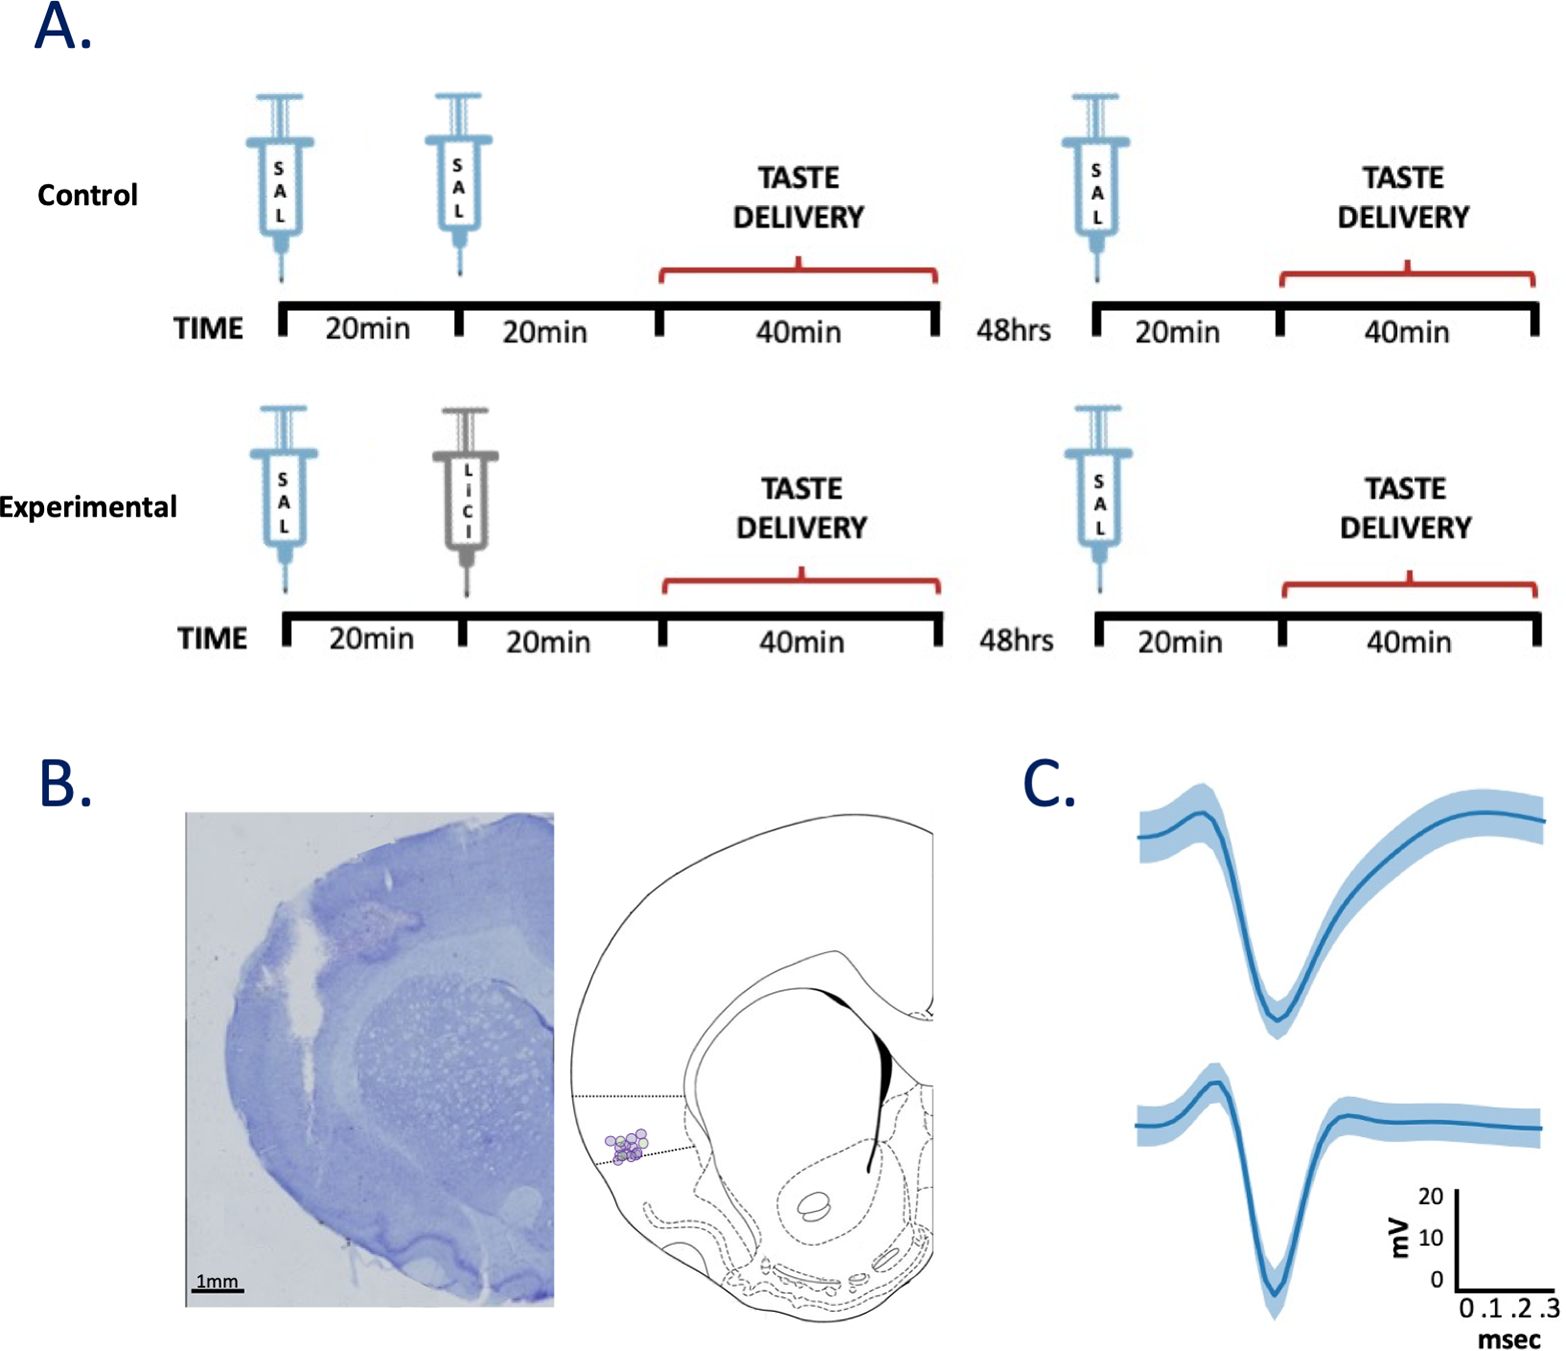
\includegraphics[width=\linewidth]{stone_2022_figs/journal.pbio.3001537.g001.png}
\caption{\textbf{General sickness induction protocol and histological verification of recording location in GC.} \textbf{(A)} On Day 1, rats received a single injection of saline followed by either an injection of saline (Control Group; top) or 0.15 M LiCl (Experimental Group, bottom). GC activity was recorded for 20 min following each injection, after which tastes were delivered via IOC across an approximately 40 min session, and 48 h later, only a single saline injection was administered to both groups, 20 min before the taste testing period. \textbf{(B)} A coronal slice (left) from 1 rat, stained with cresyl violet. The track is an electrode bundle lesion, with the end of the lesion marking the final resting location of the wires. A coronal slice schematic (right) with circles indicating the electrode bundle resting location for each rat (experiment 1: purple, experiment 2: green). \textbf{(C)} The average waveform of a representative putative pyramidal cell [top] and interneuron [bottom]. Light blue shading represents the standard deviation of the noise in the waveform. GC, gustatory cortex; IOC, intraoral cannulae; LiCl, lithium chloride.
}
\label{fig:wrapfig}
\end{figure}

\smallskip
\noindent\textbf{Water restriction}\par
\noindent 
During experimentation (Fig 2.1A), mild water restriction (ad libitum access to 20 mL every day at 4 PM, 6 h after experimental sessions), started 6 d following surgery, ensured engagement in the task. Daily records were kept of weight and water intake to ensure that rats did not fall below 85\% of presurgery weight.

\smallskip
\noindent\textbf{Experimental design}\par
\noindent 
On the second day of water restriction, rats began 2 d of habituation to liquid delivered directly to the tongue via IOC, with 60 and 120 30-\(\mu\)L infusions of water delivered each day, respectively. To maximize our ability to record from neurons held stably across both (saline and LiCl) sessions, electrodes were lowered to their recording depth (approximately 4.5 mm DV from dura) on the second day of habituation and left at that depth.

For Experiment 1, on the morning following the second habituation session, in vivo recording sessions commenced: Rats received a subcutaneous (sc; 0.50\% of body weight) injection of isotonic saline followed 20 min later by an injection of either a second saline injection (Control) or illness-inducing LiCl (Experimental; Fig 2.1A); following each injection, neural and behavioral data were collected—20 min of “passive” recording followed by 120 taste delivery trials in which 1 of 4 gustatory stimuli (0.1 M sodium chloride [NaCl], 0.3 M sucrose, 0.1 M citric acid [CA], and 0.01 M quinine-HCl [QHCl]) was delivered via IOC in a pseudo-random order. Stimuli and concentrations were chosen to ensure a range of distinct taste identities and palatabilities and to maximize comparability to our (\cite{grossman2008a,levitan2019a,moran2014a,sadacca2012a}) and others’ (\cite{spector1988a,samuelsen2012a}) studies. A second testing session, identical to the first session with the exception that only a single sc. injection of saline was administered 20 min prior to taste delivery, was given 48 h after the first testing session (Fig 2.1A), with the electrode bundle remaining in the same place. To test whether any observed LiCl/saline differences were not order effects, a subset of animals (N = 5) were subjected to the same experimental protocol with the exception of the order of injections being reversed (2 saline injections on the first day, LiCl injection on the second). Our analyses revealed no difference between the orders (ps \textgreater 0.05).

For Experiment 2, additional (N = 3) taste-naive animals were subjected to a single recording session in which the injection of LiCl was immediately followed by taste deliveries via the IOC.

\smallskip
\noindent\textbf{Illness induction}\par
\noindent 
Because we wished to elicit a mild illness that would not cause large scale, overt behaviors that might serve as confounding explanations for any observed changes in neural activity, we induced malaise using a mild concentration of LiCl (0.15 M, delivered sc). Multiple studies demonstrate that the malaise induced using this concentration is strong enough to cause conditioned taste aversion (CTAs) without causing gross changes in behavior (\cite{nachman1973a,smith1971a}).

\smallskip
\noindent\textbf{Behavioral analyses}\par
\noindent 
The assessment of lethargy provided a basic measure of sickness (\cite{parker1982a,kent1992a}). Three cameras (positioned below, above, and diagonally within the behavioral chamber (see Apparatus) captured mobility in a separate subset of animals implanted only with IOCs (N = 4 and 5, Control and Experimental). Each video was manually scored for lateral (grid-line crossings) and vertical (rears; 2 forelimb paws off the ground for \textgreater0.5 s) movements by a trained, but blind to condition, observer. Such events have been shown to be sensitive measure of welfare in rodents—healthy, nonanxious mice/rats will perform lateral and vertical movements as a means to explore their environment (\cite{nachman1975a,cross-mellor2009a}). Given the small size of the recording chamber, the rats had limited ability to move laterally, which led us to focus our analyses primarily on vertical movements. Healthy/sick differences in frequency and duration of these movements were analyzed and fit with sigmoid functions so that we could determine whether and when LiCl-treated rats became ill.

\smallskip
\noindent\textbf{Histology}\par
\noindent 
At the completion of the experiment, rats were deeply anesthetized with ketamine/xylazine (200:20 mg/kg, IP) and then perfused transcardially with physiological saline followed by 10\% formalin. The brains were extracted and stored in a 10\% formalin/30\% sucrose solution for at least 3 d before staining, after which they were frozen and sliced on a sliding microtome (Leica SM2010R, Leica Microsystems; thickness 60 \(\mu\)m). Slices were mounted, and sections were stained with a Nissl stain (Thermo Fisher Scientific, Indianapolis, IN) to evaluate cannulae and electrode tracks, respectively, via inspection of fluorescence on a light microscope (Fig 2.1B).

\smallskip
\noindent\textbf{Electrophysiology methods and analyses}\par
\noindent 
Differential recordings from the micro-electrodes were sampled at 30 kHz using a 32-channel analog-to-digital converter chip (RHD2132) from Intan Technologies. The signals were digitalized online at the head stage/amplifier and saved to the hard drive of the PC. The collected recordings were filtered for either single-neuron action potential isolation (300 to 3,000 Hz bandpass) or LFPs (1 to 300 Hz lowpass) and analyzed off-line. Putative single-neuron waveforms (3:1 signal-to-noise ratio) were sorted using a semi-supervised methodology: Putative action potentials were grouped into clusters by a Gaussian mixture model (GMM) with strict noise tolerance and refined manually; conservatism was enhanced via a requirement that the variability in spiking be random (and thus not reflecting biased cluster cutting; for the details of the recording system and Python scripts, see \cite{mukherjee2017a}). To further ensure that the isolated waveforms represented single-neuron records, we also calculated the interspike intervals and removed units for which \(\ge\)1\% of the intervals disobeyed the biological constraints of refractory period. By this approach, a total of 266 and 190 GC neurons were isolated from, respectively, 7 Experimental (saline-LiCl) and 5 Control (saline-saline) rats across 24 sessions (2 sessions/animal).

All analyses, unless otherwise stated, were performed using all neurons; in a few cases (noted in the text), analysis was restricted to neurons that were taste responsive (see also Table 1.1 below).

\begin{tablular}
\centering
    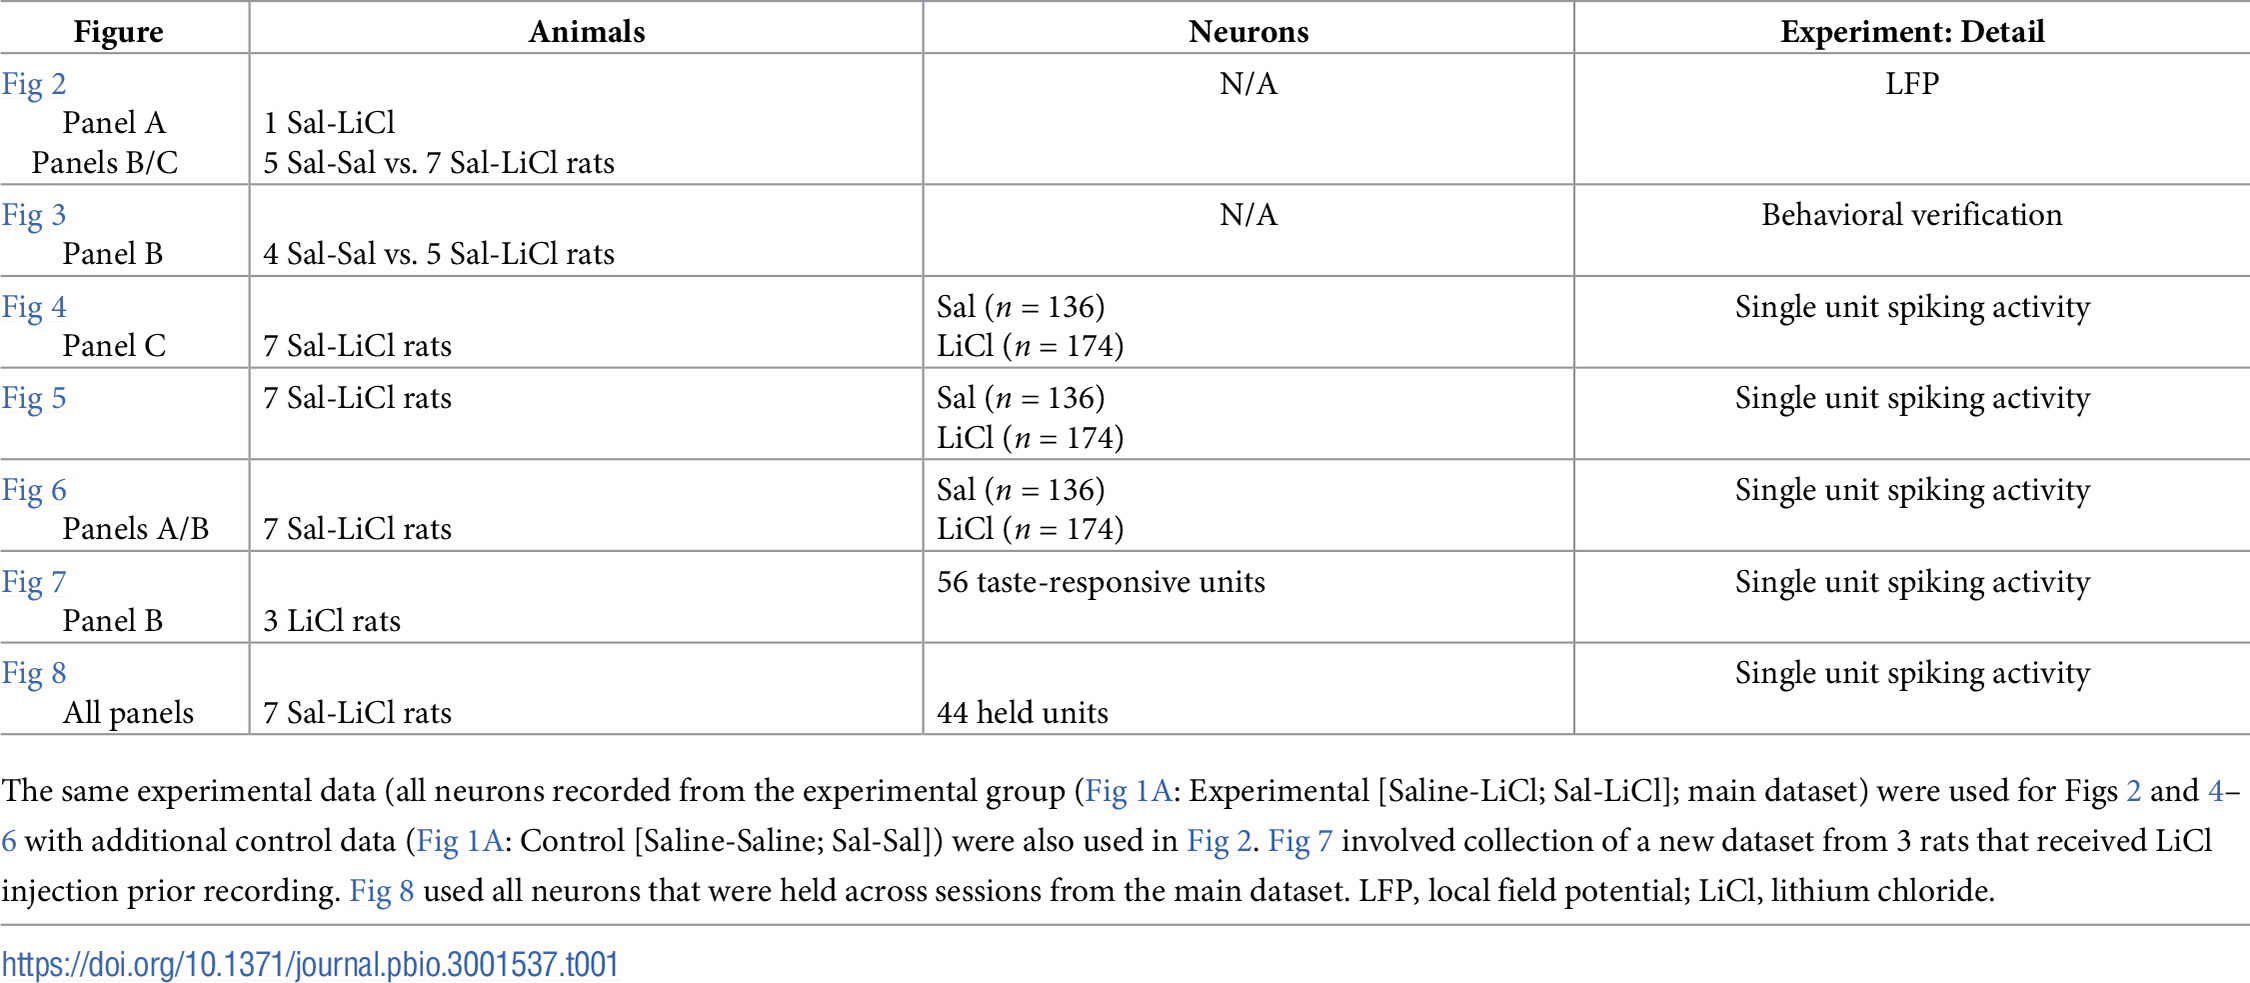
\includegraphics[width=\linewidth]{stone_2022_figs/journal.pbio.3001537.t001.png}
\end{tablular}

LFPs were extracted only from channels containing isolated single-neuron data, in order to avoid potential signal artifact arising from noisy/broken channels. Data were averaged across electrodes within and across session for each animal, and analyzed across the 1 to 20 Hz frequency bands, with focus on the \(\mu\) bands (7 to 12 Hz, (\cite{tort2010a,tort2010b,thomson1991a}) in 1-min time bins). After normalizing (across the entire session) each animal’s \(\mu\) power to between 0 and 1, the LiCl vectors were subtracted from the saline vectors to reveal changes in \(\mu\) following LiCl administration, and an ANOVA was used to compare groups. Differences were considered significant only if 3 or more consecutive time bins reached a p \textless 0.05 criterion.

\smallskip
\noindent\textbf{Changepoint analysis}\par
\noindent 
To determine the position of a change point in GC \(\mu\) power, we used a custom model implemented in the PyMC3 probabilistic programming package (\cite{salvatier2016a}), with parameter estimation performed using Markov Chain Monte Carlo sampling (see details below). The LFP power time series were z-scored, and then modeled using 2 normal distributions; the model attempts to detect a single change point (\(\tau\)) in the mean value of the LFP power as the time series switches between distributions. Change points were determined for each animal independently.

$$ \textrm{LFP Power Mean} : \(\mu\)_1,\(\mu\)_2 \sim  \mathcal{N}(0,1) $$
$$ \textrm{LFP Power Variance} :\(\sigma\) \sim \text{HalfCauchy}(1) $$
$$ \textrm{Changepoint Position} : \(\tau\) \sim \text{Uniform}(0,20) $$
$$
 \textrm{Observed LFP Power} : \text{Obs}(t) \sim \begin{cases}
    \mathcal{N}(\(\mu\)_1,\(\sigma\)), &  t\textless\(\tau\)\\
    \mathcal{N}(\(\mu\)_2,\(\sigma\)), &  t\(\ge\)\(\tau\)
  \end{cases}
$$

Since sampling returns a distribution over the parameter values explaining the data, distributions of \(\tau\) with low variance (high peaks) indicate strong presence of a change point. To mark the position of these change points using the \(\tau\) distribution in an unbiased manner, we compared the \(\tau\) distributions (containing equal numbers of samples) of our time series (actual data) to those of 50 temporally shuffled time series (shuffled data), which, by definition, have no change points. Points in the actual data distribution higher than the 99th percentile of the shuffle distribution were marked. The average of these marked time points was taken to be the position of the change point for that time series.

The calculation of the behavioral changes and LFP change points was performed on separate cohorts of animals. We then quantified the likelihood that the close synchronization between the behavioral and neural changes seen in our data could have happened by chance, by comparing the data to simulated data produced under the assumption that the latencies of the average behavioral and LFP change points are drawn from independent, uniform distributions. We calculated the distribution of summed, absolute distances between the behavioral and LFP change points, testing the hypothesis that the change points in our data are clustered more tightly than those drawn from the simulation (a p-value less than 0.05 indicates a significantly more coupled relationship than if time points were truly independent).

\smallskip
\noindent\textbf{Taste responsiveness}\par
\noindent 
We defined basic responsiveness to taste delivery by first subtracting the across-trial averaged 1 s of prestimulus firing from the first 1 s of taste-evoked firing for each neuron (ignoring the first 200 ms of post-taste activity; see below), and subjecting the resultant single-neuron data to a Mann–Whitney U test to determine whether a significant change in firing rate occurred when the taste hit the tongue. These data were then pooled to ascertain the overall magnitude of response change under different conditions. But because taste delivery could reduce firing to below baseline levels in some neurons (thereby masking the true magnitude of effects in the averaging of enhanced and reduced firing rates), we divided the sample into those in which firing normalized to pre-stimulus baseline was greater than zero, and those in which it was less than zero. We refer to these as “excitatory” and “inhibitory responses,” respectively, but note that this designation only refers to the direction of firing rate change—we make no claims regarding whether or not “inhibitory responses” are caused by direct inhibitory influence on these neurons; nor do we intend to imply that these are responses found in inhibitory interneurons. We used a 2-way ANOVA to test whether LiCl administration changed taste response magnitude.

Note that in these analyses, as well as in those described below, we typically ignored the first 200 ms of post-taste activity. This was done because we have repeatedly observed that these early responses are seldom chemosensory in our paradigm, reflecting only tactile stimulation of the tongue (see \cite{fontanini2006a,katz-a,katz2001a,sadacca2016a,sadacca2012a,jones2007a}. This differentiates our paradigm from those in which rats perform active licking or lever-pressing for fluid delivery (\cite{gutierrez2010a,stapleton2006a,graham2014a,bouaichi2020a,dikecligil2020a}), wherein researchers observe a much shorter pre-chemosensory response, likely because the rodent is able to anticipate taste acquisition (see also \cite{li2016a}).

\smallskip
\noindent\textbf{Taste specificity}\par
\noindent 
The above analysis is performed on data averaged across tastes, and therefore serves only to estimate whether, and how, GC is responsive to oral stimuli—not whether that response depends upon stimulus identity. To determine how LiCl impacted the taste specificity of GC responses, we subjected whole ensembles to a standard linear discriminant analysis (LDA) classifier used in previous studies (\cite{katz2001a,sadacca2016a,nicolelis1997a}). This classifier tests the reliability with which a trial of taste-evoked responses in an ensemble of simultaneously recorded neurons can be identified among responses to other tastes. We binned neural responses into 250 ms bins and used a linear classifier with a leave-one-out validation approach, calculating the prediction accuracy of the classifier averaged across each excluded trial for each time bin. Paired-sample t tests (with Bonferroni correction) were performed for each post-taste delivery epoch (see above) to determine the impact of LiCl.

To assess changes of taste discriminability within a single session, the ensemble-wise LDA classifier was trained on the first 5 trials (per taste) and tested on later trials. Here, and when testing the degree to which sickness impacted discriminability in real-time, we restricted the analysis to taste-responsive units (typically \textgreater70\% of the total number of recorded neurons [\cite{katz-a,katz2001a,jones2007a}]; see Table 1.1): Across-iteration averages were computed for each tested trial and the resulting means were binned into 5-trial blocks (approximately 6 min/block). Blocks were normalized (between 0 and 1) across animals, and results were subject to a repeated measures ANOVA and a series of paired-sample t tests (with Bonferroni correction).

Finally, it is worth noting that taste responsiveness and taste specificity provide slightly different types of information about GC activity. It is possible for a neuron to be taste responsive and not respond distinctly to different tastes, and it is possible for a neuron to respond in a manner that is taste specific without the average, across-stimuli response being significantly modulated from baseline. Both are useful.

\smallskip
\noindent\textbf{Taste palatability}\par
\noindent 
Using our now-standard palatability-correlation analysis (\cite{sadacca2016a,moran2014a,li2016a,piette2012a}), we evaluated the degree to which LiCl altered the amplitude of palatability-relatedness in late epoch GC taste responses. Using a moving window (window size: 250 ms, step: 25 ms), we correlated firing rates with well-established palatability ranks (sucrose \textgreater NaCl \textgreater CA \textgreater QHCl; [\cite{sadacca2016a,li2013a}]) and compared the magnitude of this correlation in healthy and sick rats.

In a further analysis of palatability-relatedness, we computed what we termed a “pure palatability index” (PPI), adapting methods from (\cite{fontanini2009a}) to test the degree to which GC taste responses could be described to code a simple “good versus bad” dichotomy. Specifically, we compared the Euclidian distances between single neurons’ responses (normalized to -500 ms pre-taste delivery) to tastes with similar palatability (i.e., sucrose and NaCl, CA and QHCl) to those between tastes with different palatability (sucrose and CA, sucrose and QHCl, NaCl and CA, NaCl and QHCl). This amounts to evaluating the ratio of the distances between “different-palatability” and “same-palatability:” a lack of palatability-related information results in a PPI of 0 (because tastes of similar palatability and tastes of different palatabilities are equally distant from one another); the more polarized the response into “good versus bad”—the larger the ratio—the more positive the PPI. To avoid artificially attenuating the effect via the inclusion of information from different epochs in single averages, the PPI was calculated from firing within the middle of our standard epochs (\cite{katz-a,katz2001a}). The results were significance tested using a Wilcoxon test.

We hasten to emphasize that these analyses of the degree to which firing is palatability-related are quite different from the above-described analysis of the degree to which firing is taste specific. In fact, taste information and palatability-relatedness are actually very different variables—one makes use of any cell-specific differences in responses to different tastes, and one is specifically measuring whether a particular pattern of responsiveness exists—necessitates these differences in analysis.

\smallskip
\noindent\textbf{Stability of single-neuron waveforms across days}\par
\noindent 
A subset of analyses required the stable tracking of neurons held across testing sessions (i.e., “held neurons,” Table 1.1). To evaluate whether a neuron was “held,” we performed a spike shape analysis the likes of which has been brought to bear in several previous studies (\cite{grossman2008a,moran2014a,nicolelis2003a,herry2008a}). We applied a conservative criterion for stability based on within-session data (comparing each neuron’s waveforms from the first third of the session to those of the last third)—only neurons for which the between-session (nonparametric clustering statistic) value was less than the 95th percentile value calculated from the within-session data were deemed to have been stably held. Of the entire population of recorded GC neurons, a total of 44 (23.2\%) satisfied this criterion.

\smallskip
\noindent\textbf{Cluster detection in patterns of healthy-ill response differences}\par
\noindent 
A clustering analysis was used to identify groups of held neurons for which LiCl impacted palatability-related firing similarly. A condition response was determined for each held unit (under each condition) by taking the average (minmax-normalized) pre- (-750$\rightarrow$250 ms) and post-delivery (250$\rightarrow$750 ms) firing rates (presented as a percentage of maximum responsiveness). We then calculated and plotted the distance and Cartesian direction between condition responses or each neurons’ taste response, yielding 176 (44 held units × 4 tastants) response differences (RDs)—quantification of how LiCl administration changed the excitatory or inhibitory response to the taste. As a conservative estimate of RD likeness, we determined the number of clusters that best fit a GMM probability distribution (calculating the Bayesian information criterion) as done previously (\cite{athey2019a}). Classifications were considered valid only if they fell within the 95\% confidence interval from the centroid of each respective cluster (see Fig 2.8D), after which we constrained our analyses to neurons within the same cluster.

\smallskip
\noindent\textbf{Cluster-specific taste palatability}\par
\noindent 
Using methods described above, we evaluated the effect of LiCl administration on palatability-related firing for neurons within clusters. A nonparametric 2-way ANOVA was used to reveal whether differences (saline–LiCl) in hedonic coding (Spearman rho$^2$) differed across cluster and time during taste processing.

\section{Results}
\subsection{LiCl administration changes GC LFPs and behavior}
We recorded activity for 20 min following subcutaneous injections of either LiCl or saline, before beginning to record taste-driven activity (Fig 2.1A); GC single-unit responses (Fig 2.1C) and LFPs were acquired from drivable bundles of 32 wires. Given that network function, measured in terms of spectral properties of LFPs, appears to change with even the most innocuous of body states (e.g., sleep versus wake, (\cite{mukamel2014a,ab2015a}), and that single-neuron firing is altered in concert with these changes (\cite{manning2009a,fontanini2008a}), our investigation into the characterization of illness started with assessment of changes in GC LFPs. We focused on power in the mu (\(\mu\): 7 to 12 Hz; \cite{fontanini2005a}) range, because power in this frequency band has proven particularly sensitive to changes in even general states related to wakefulness and attention (\cite{ching2014a,fontanini2005a,fontanini2006a,tort2010a,vijayan2013a}). While the results described below were also observed in frequency ranges above (e.g., \(\beta\)) and below (i.e., \(\theta\)) \(\mu\), they were centered on and largest in the \(\mu\) range.

Save for the brief period immediately following handling and injections, the amplitude of \(\mu\) in the LFPs remained relatively stable across the first half of the (20 min) post-injection recording periods for both experimental groups, but an impact of LiCl injections emerged in the second 10-min period following injections for the saline-LiCl group (Fig 2.2A: LFPs spectral power from a representative rat following either saline [top] or LiCl injection [bottom]). The precise nature of this impact varied with individual, in some cases (N = 3) involving a reduction of \(\mu\) power and in some cases an increase (N = 4), but a change point analysis quantifying the time points and likelihoods of change in \(\mu\) power for each animal (across both experimental groups) revealed that LiCl-induced changes in GC \(\mu\) power reached significance at around the same time in the majority (5 out of 7) rats (Fig 2.2B, bottom). That is, the timing of the change in spectral properties was remarkably reliable across the 7 rats, despite the fact that in some cases the change involved an enhancement of the power in the \(\mu\) range, and in some cases the opposite: had no change occurred, or had the change been gradual/subtle following injection (as in saline-saline–injected rats, Fig 2.2B, top, N = 5), the likelihood of change (\(\tau\); posterior distribution) would be spread uniformly across post-injection time; instead, the analysis reveals that a change in GC \(\mu\) power reliably occurs between 10.89 and 17.07 min post-injection (never before and never after), with the mean likelihood occurring at 15.11 min.

\begin{figure}
\centering
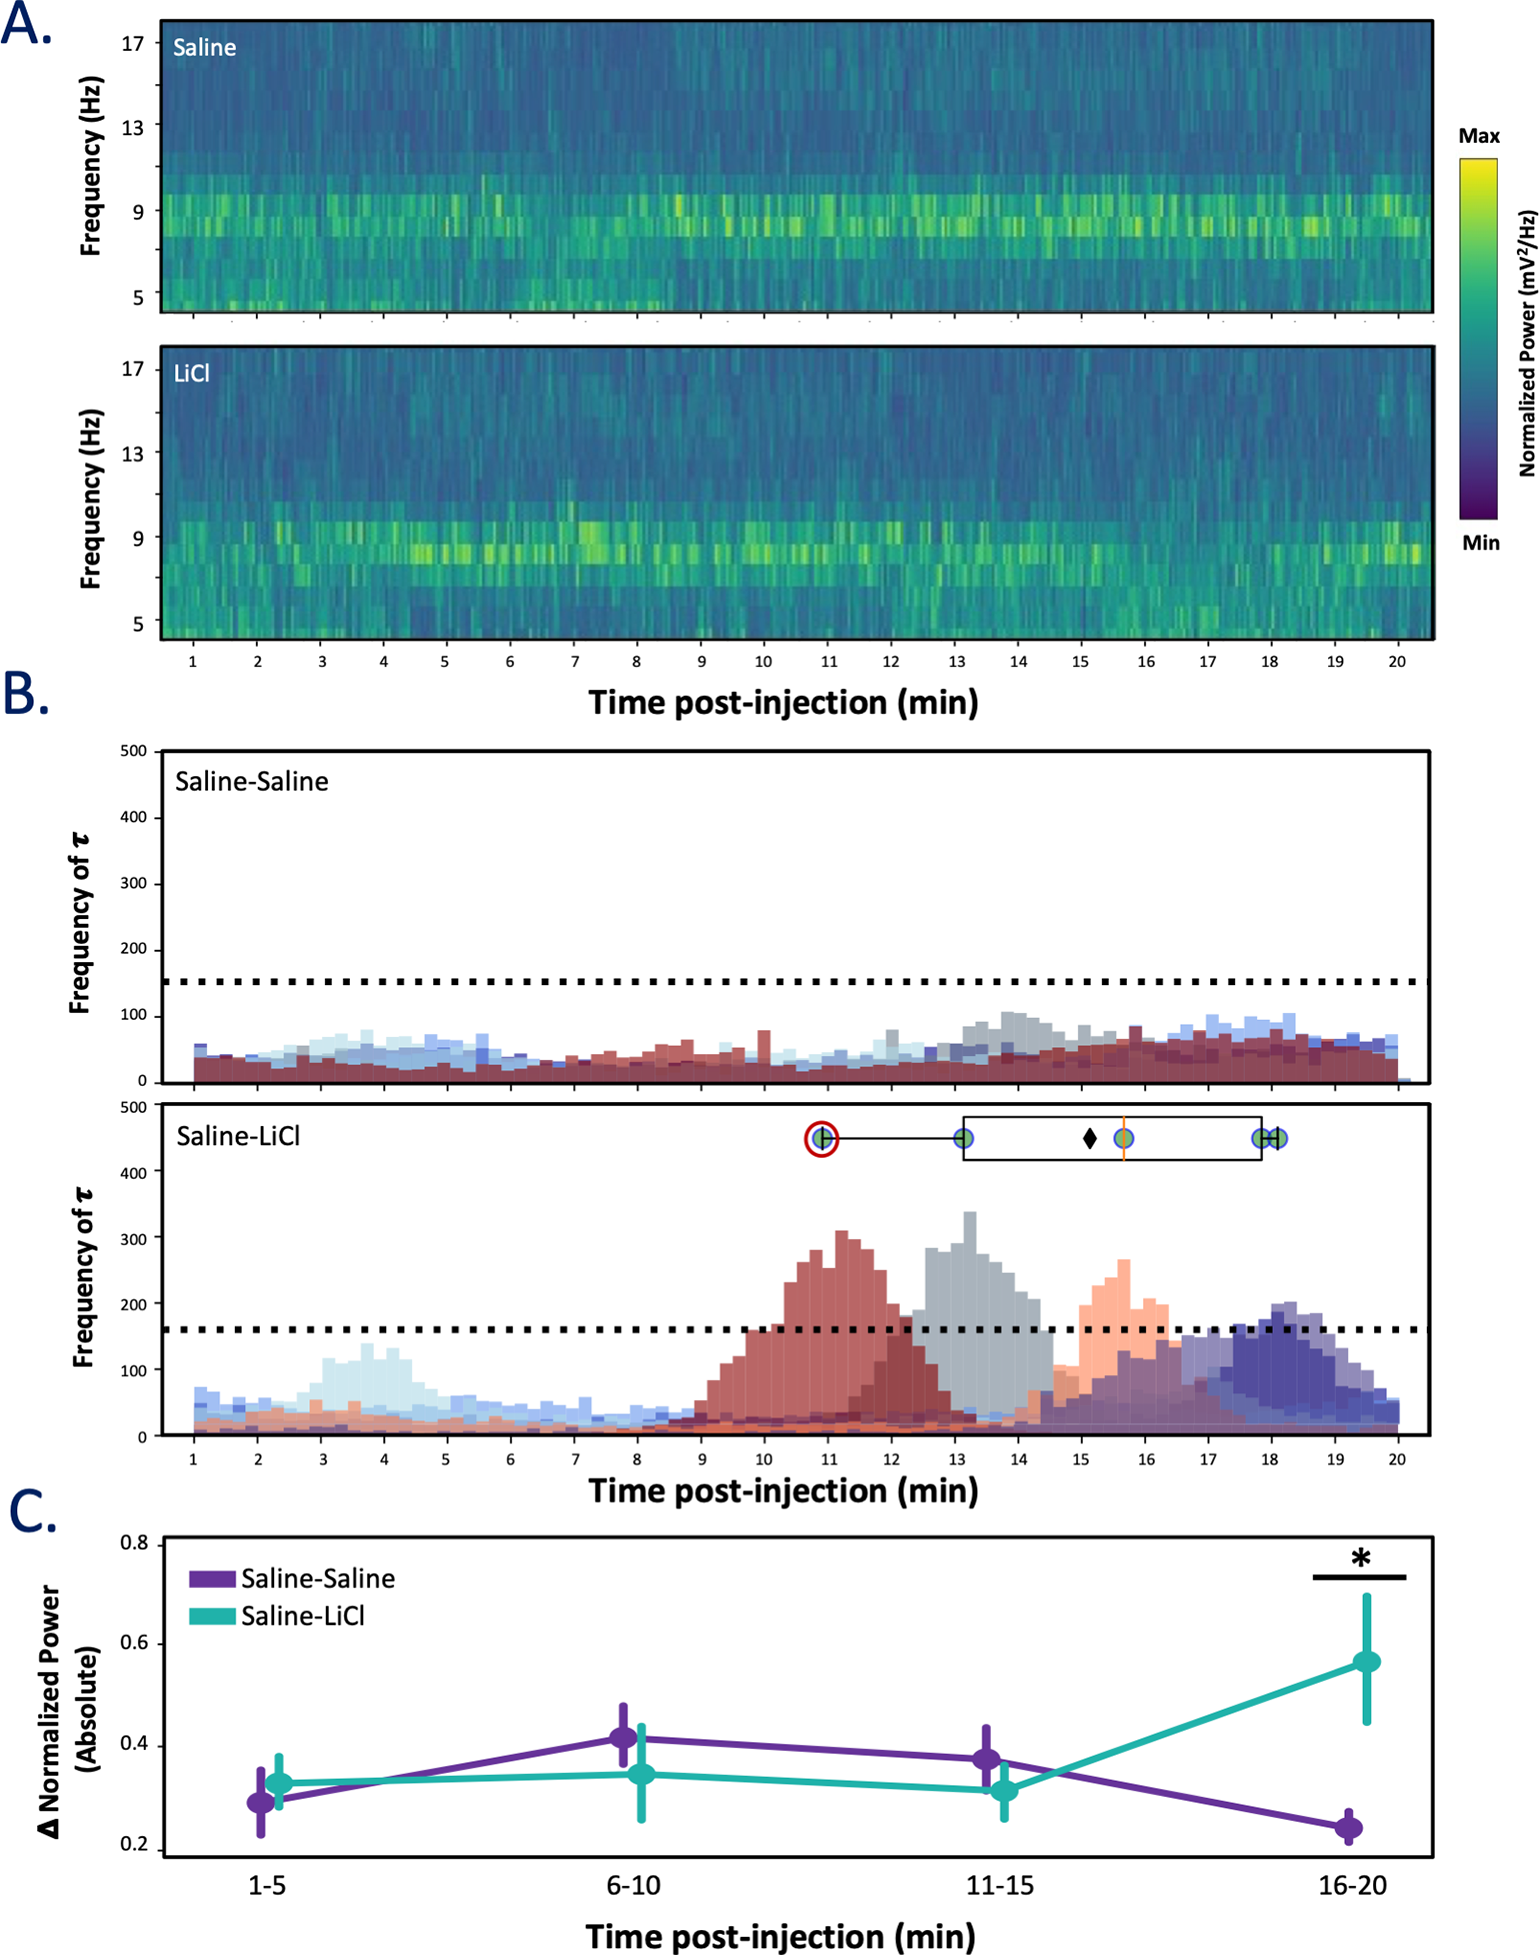
\includegraphics[width=0.7\linewidth]{stone_2022_figs/journal.pbio.3001537.g002.png}
\caption{\textbf{LiCl administration alters GC LFP 15-min post-injection.} \textbf{(A)} Representative spectrograms from 1 animal (saline-LiCl condition) showing activity after saline (top) or LiCl (bottom) injection. LiCl reduces power in μ during the last half of the 20-min period. \textbf{(B)} The posterior distributions for a single change point model identify the probabilities of a change (shown as frequency of \(\tau\)) in μ power (each color represents distribution for single animal) for saline-saline (top, N = 5) and saline-LiCl (bottom, N = 7) groups. The horizontal dashed lines indicate the 99th percentile from temporally shuffled data, and the overlaid boxplot depicts the range in peak likelihood of change in μ power for distributions with values higher than the 99th percentile: Each dot represents a single animal (the animal from panel A is noted with a red circle); the box extends from the lower to upper quartiles (red line: median, black diamond: mean) of likelihood. The mean onset of the change in μ power occurs at 15.11 min, with all change points occurring after 10-min post-injection and before 18-min post-injection. \textbf{(C)} The absolute difference in μ for saline-saline (purple) and saline-LiCl (teal) groups reveals a significant interaction between change in μ power and quartile (p \textless 0.05, 2-way ANOVA), with LiCl changing μ power significantly within the fourth quartile (* p \textless 0.05; 1-way ANOVA). The error bars represent SEMs. LFP, local field potential; LiCl, lithium chloride.
}
\label{fig:wrapfig}
\end{figure}

An analysis of the group data confirms these rat-by-rat results, demonstrating that absolute changes in \(\mu\) power following LiCl injection emerged late in the 20-min post-injection recording session (compared to saline-saline animals, Fig 2.2C). A 2-way ANOVA on these data revealed a significant interaction between group and quartile (F(3, 33) = 3.62, p = 0.023); a subsequent 1-way ANOVA confirmed that the absolute difference reached significance only in the 16 to 20-min post-injection bin (F(1, 11) = 5.14, p = 0.04) for the saline-LiCl group. While in some cases, an apparent change in spectral power (in this case, \(\mu\) power) could in fact be an artifactual effect of firing rate changes (\cite{waldert2013a}), our investigation failed to observe concomitant changes in firing rate at any time across the 20-min post-injection recording session (F(3, 33) = 2.39, p = 0.09; see also Fig 2.8A); this suggests that our observed effect on \(\mu\) is not simply a reflection of firing rate change, but rather a matter of network synchrony being modulated.

Overall, these results accord well with those of previous studies, in that they demonstrate: (1) that changes in LFP activity are hallmarks of the onsets of cortical state changes, regardless of the specific directionality of the changes (\cite{pachitariu2015a,zhou2014a,tan2014a,zucca2019a}); and (2) that sickness-related behaviors such as immobility emerge at approximately this time point following LiCl injections (\cite{nachman1975a,cross-mellor2009a,parker2004a,tomasiewicz2006a,l2019a,smith1978a}).

To more completely test this last point, we compared our LFP data to (independently collected and blindly coded) video recordings of illness-related behaviors, predicting that the above-described changes in network activity would roughly coincide with times at which changes in mobility appeared following LiCl injections. Because we specifically injected a low concentration of LiCl in order to avoid gross movement changes that could confound interpretation, and because the small recording chamber limited the rats’ ability to move laterally, we focused our measurement of mobility on rearing events in which the animal lifted both forepaws off the floor simultaneously without proceeding to grooming (\cite{grill1978a,grill1978b}). We specifically hypothesized that reduction of such rearing events, which has been linked to mild LiCl-induced illness (\cite{smith1978a}), would occur at around the time that we observed changes in cortical LFP \(\mu\) power (Fig 2.3A).

\begin{figure}
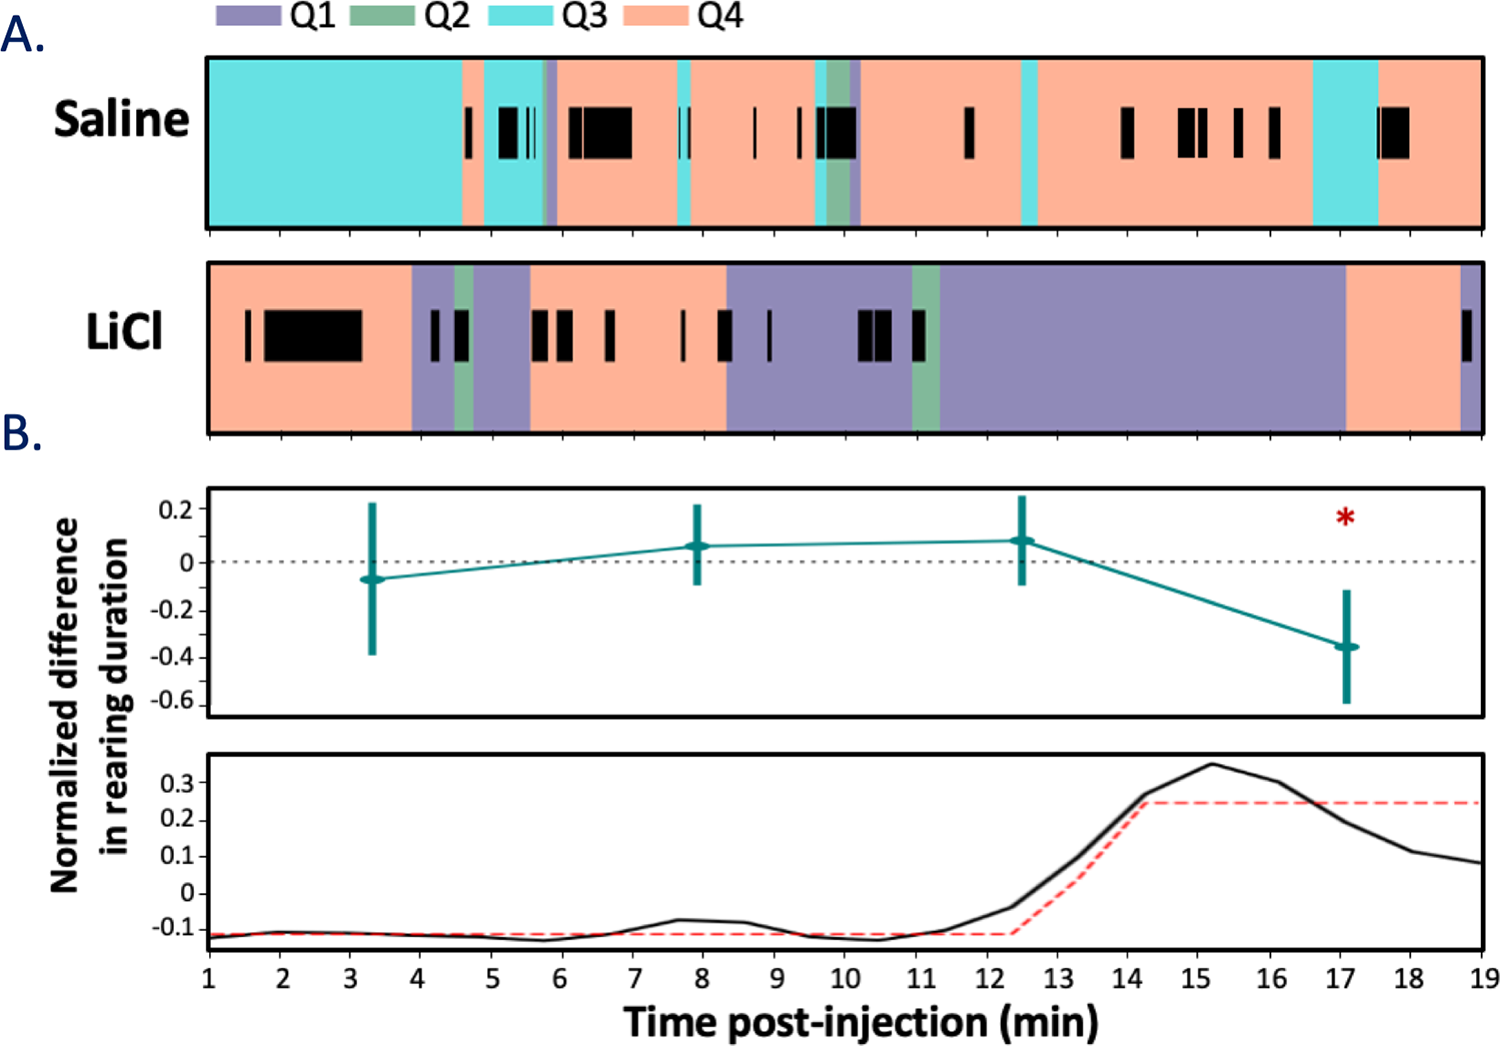
\includegraphics[width=\linewidth]{stone_2022_figs/journal.pbio.3001537.g003.png} 
\caption{\textbf{LiCl administration reduces rearing approximately 12 min after LiCl injection.} \textbf{(A)} An example rat’s movement through time around the cage space (color coding shows the rat’s position in the box, Quadrant 1–4) overlain with rearing (black bars) durations after saline (top) and LiCl injections (bottom). \textbf{(B)} The average normalized LiCl–saline difference in rearing duration across animals (N = 4 and 5, saline and LiCl) reveals (top) a significant reduction of rearing occurring in the fourth quarter of the session (* p \textless 0.05, Wilcoxon-rank sum). A more fine-grained analysis (bottom) suggests that the change in behavior (black line) begins at 12-min post-injection; the dashed red line illustrates the sigmoidal fit (r$^2$ = 0.72). The error bars represent SEMs. LiCl, lithium chloride.
}
\label{fig:wrapfig}
\end{figure}



In fact, the durations of rearing events declined following LiCl (N = 5) injection, but not following saline injection (N = 4). A 2-way repeated measures ANOVA brought to bear on the 20-min recording session (again binned into 5 min quartiles to ensure sufficient power; Fig 2.3B, top) revealed a significant difference in rearing duration emerging post-injection (F(3, 182) = 3.14, p \textless 0.05)—a change that, like the change in cortical LFP power, became significant (according to post hoc Wilcoxon signed-rank tests) only in the 15- to 20-min post-injection bin (W = 158, Z = 0.65, p = 0.024, r = 0.50), compared to rats receiving only saline injections.

A sigmoidal curve fit to the normalized LiCl-saline difference in rearing duration (Fig 2.3B, bottom) confirmed that the appearance of this illness-related change in behavior (the asymptote minima of fit; r$^2$ = 0.72) aligned well with the above-noted change in GC \(\mu\) power (compared to Fig 2.2, top), again suggesting that the onset of LiCl-induced illness is reflected in the function of the GC network. The fact that the Figs 2.2 and and 2.3 data were collected from separate groups of rats only increases the conservatism of this interpretation—the likelihood that this close alignment of behavioral and neural changes would occur if LFP change points of the first cohort and behavioral change points of the second cohort were random (uniformly distributed) and uncoupled is extremely low (difference between real and modeled data, p = 0.03). While this result does not conclusively rule out the possibility that LiCl could independently cause illness and cortical changes (see Discussion), the pattern of results implicates the emergence of illness (as reflected in behavior) in the change in GC spectral properties.

\subsection{LiCl administration causes GC taste responses to collapse into a “good-bad” distinction between tastes}
Fig 2.4A shows 2 example of GC single-neuron taste responses—one for which taste administration caused inhibitory firing rate changes, one excitatory—from each type of session (saline/healthy and LiCl/illness). As an initial look at how illness impacts these responses, we evaluated the magnitudes of responses elicited by tastes delivered directly into the mouth via IOC. While initial paired-sampled t tests (with Bonferroni correction for multiple comparisons) performed across the entire pooled sample failed to reveal an impact of LiCl, this apparent non-effect proved to be an artifact of averaging across neurons with “excitatory” and “inhibitory” taste responses: When we performed separate analyses of those 2 types of taste responses, it became clear that LiCl-induced illness reduced the magnitude of both excitatory and inhibitory GC taste responses (Fig 2.4B). A 2-way ANOVA performed on these data revealed a significant interaction between the condition and taste response direction (F(1,3191) = 6.05, p = 0.014); a Tukey post hoc comparison showing the main effect of illness was larger for excitatory responses (p = 0.003) but not for inhibitory responses (p \textgreater 0.05).


\begin{figure}
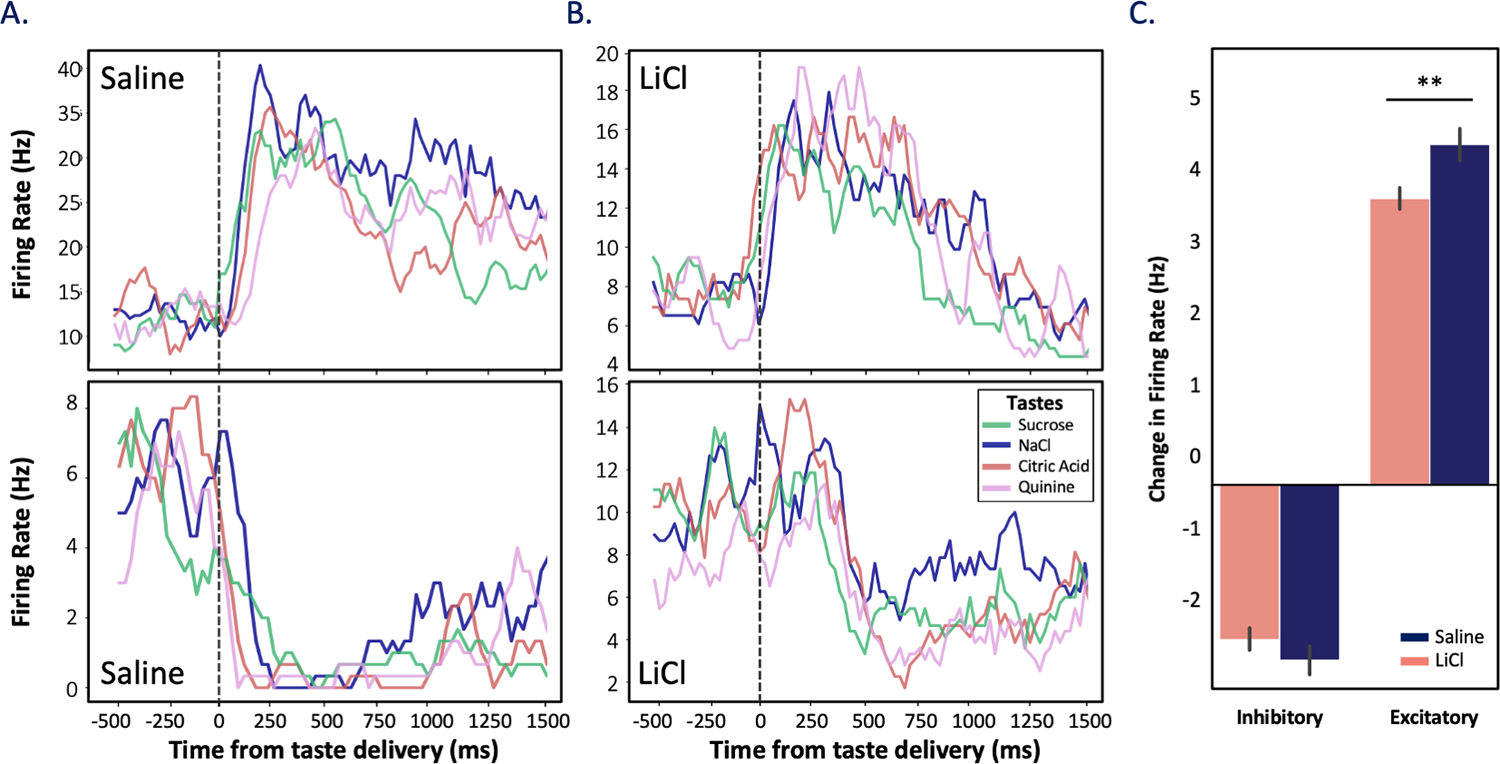
\includegraphics[width=\linewidth]{stone_2022_figs/journal.pbio.3001537.g004.png} 
\caption{\textbf{LiCl administration reduces magnitudes of taste responsiveness}. PSTHs of trial-averaged firing rates of 4 representative neurons recorded in \textbf{(A)} saline and \textbf{(B)} LiCl states. The examples in the top panels show excitatory responses, and the bottom examples show inhibitory responses. Vertical dashed lines indicate the time of taste delivery. Subtle variances in firing rates observed between 0–200 ms are not statistically significant (1-way ANOVA, ps \textgreater 0.05, see Methods). \textbf{(C)} Illness decreased the magnitude of these responses; for neurons with excitatory responses, this reduction was significant (** p \textless 0.01; 2-way ANOVA with Tukey post hoc). Error bars represent SEMs across neurons. LiCl, lithium chloride; PSTH, peristimulus time histogram.
}
\label{fig:wrapfig}
\end{figure}


The above analysis, however, examines only responsiveness, providing no information regarding whether the impact of LiCl-induced illness differs for different specific tastes. We therefore performed an LDA, quantifying the reliability with which GC responses to one taste could be differentiated from responses to other tastes. As shown in Fig 2.5 (blue trace and bars below), LDA enables us to correctly identify administered tastes from middle epoch responses on over 40\% of the trials in healthy sessions (well above chance, which = 25\%); this percentage quickly rises to over 50\%, despite the use of a small time bin sliding window analysis that left the data at the mercy of unsmoothed trial-to-trial variability. More to the point, this distinctiveness (i.e., classifiability) of responses was significantly diminished following systemic LiCl administration (coral trace and bars in Fig 2.5), with the decrement becoming significant in the “middle epoch” and continuing into the “late epoch” (Mann–Whitney U (1-tailed) = 1,952, M = 34.06\%/43.77\%, SD = 11.09\%/14.58\%, p = 0.0003; U = 2,045, M = 39.78\%/47.83\%, SD = 15.72\%/14.64\%, p = 0.001, respectively). Taste responses carry less identity-related information when the rat is ill.

\begin{figure}
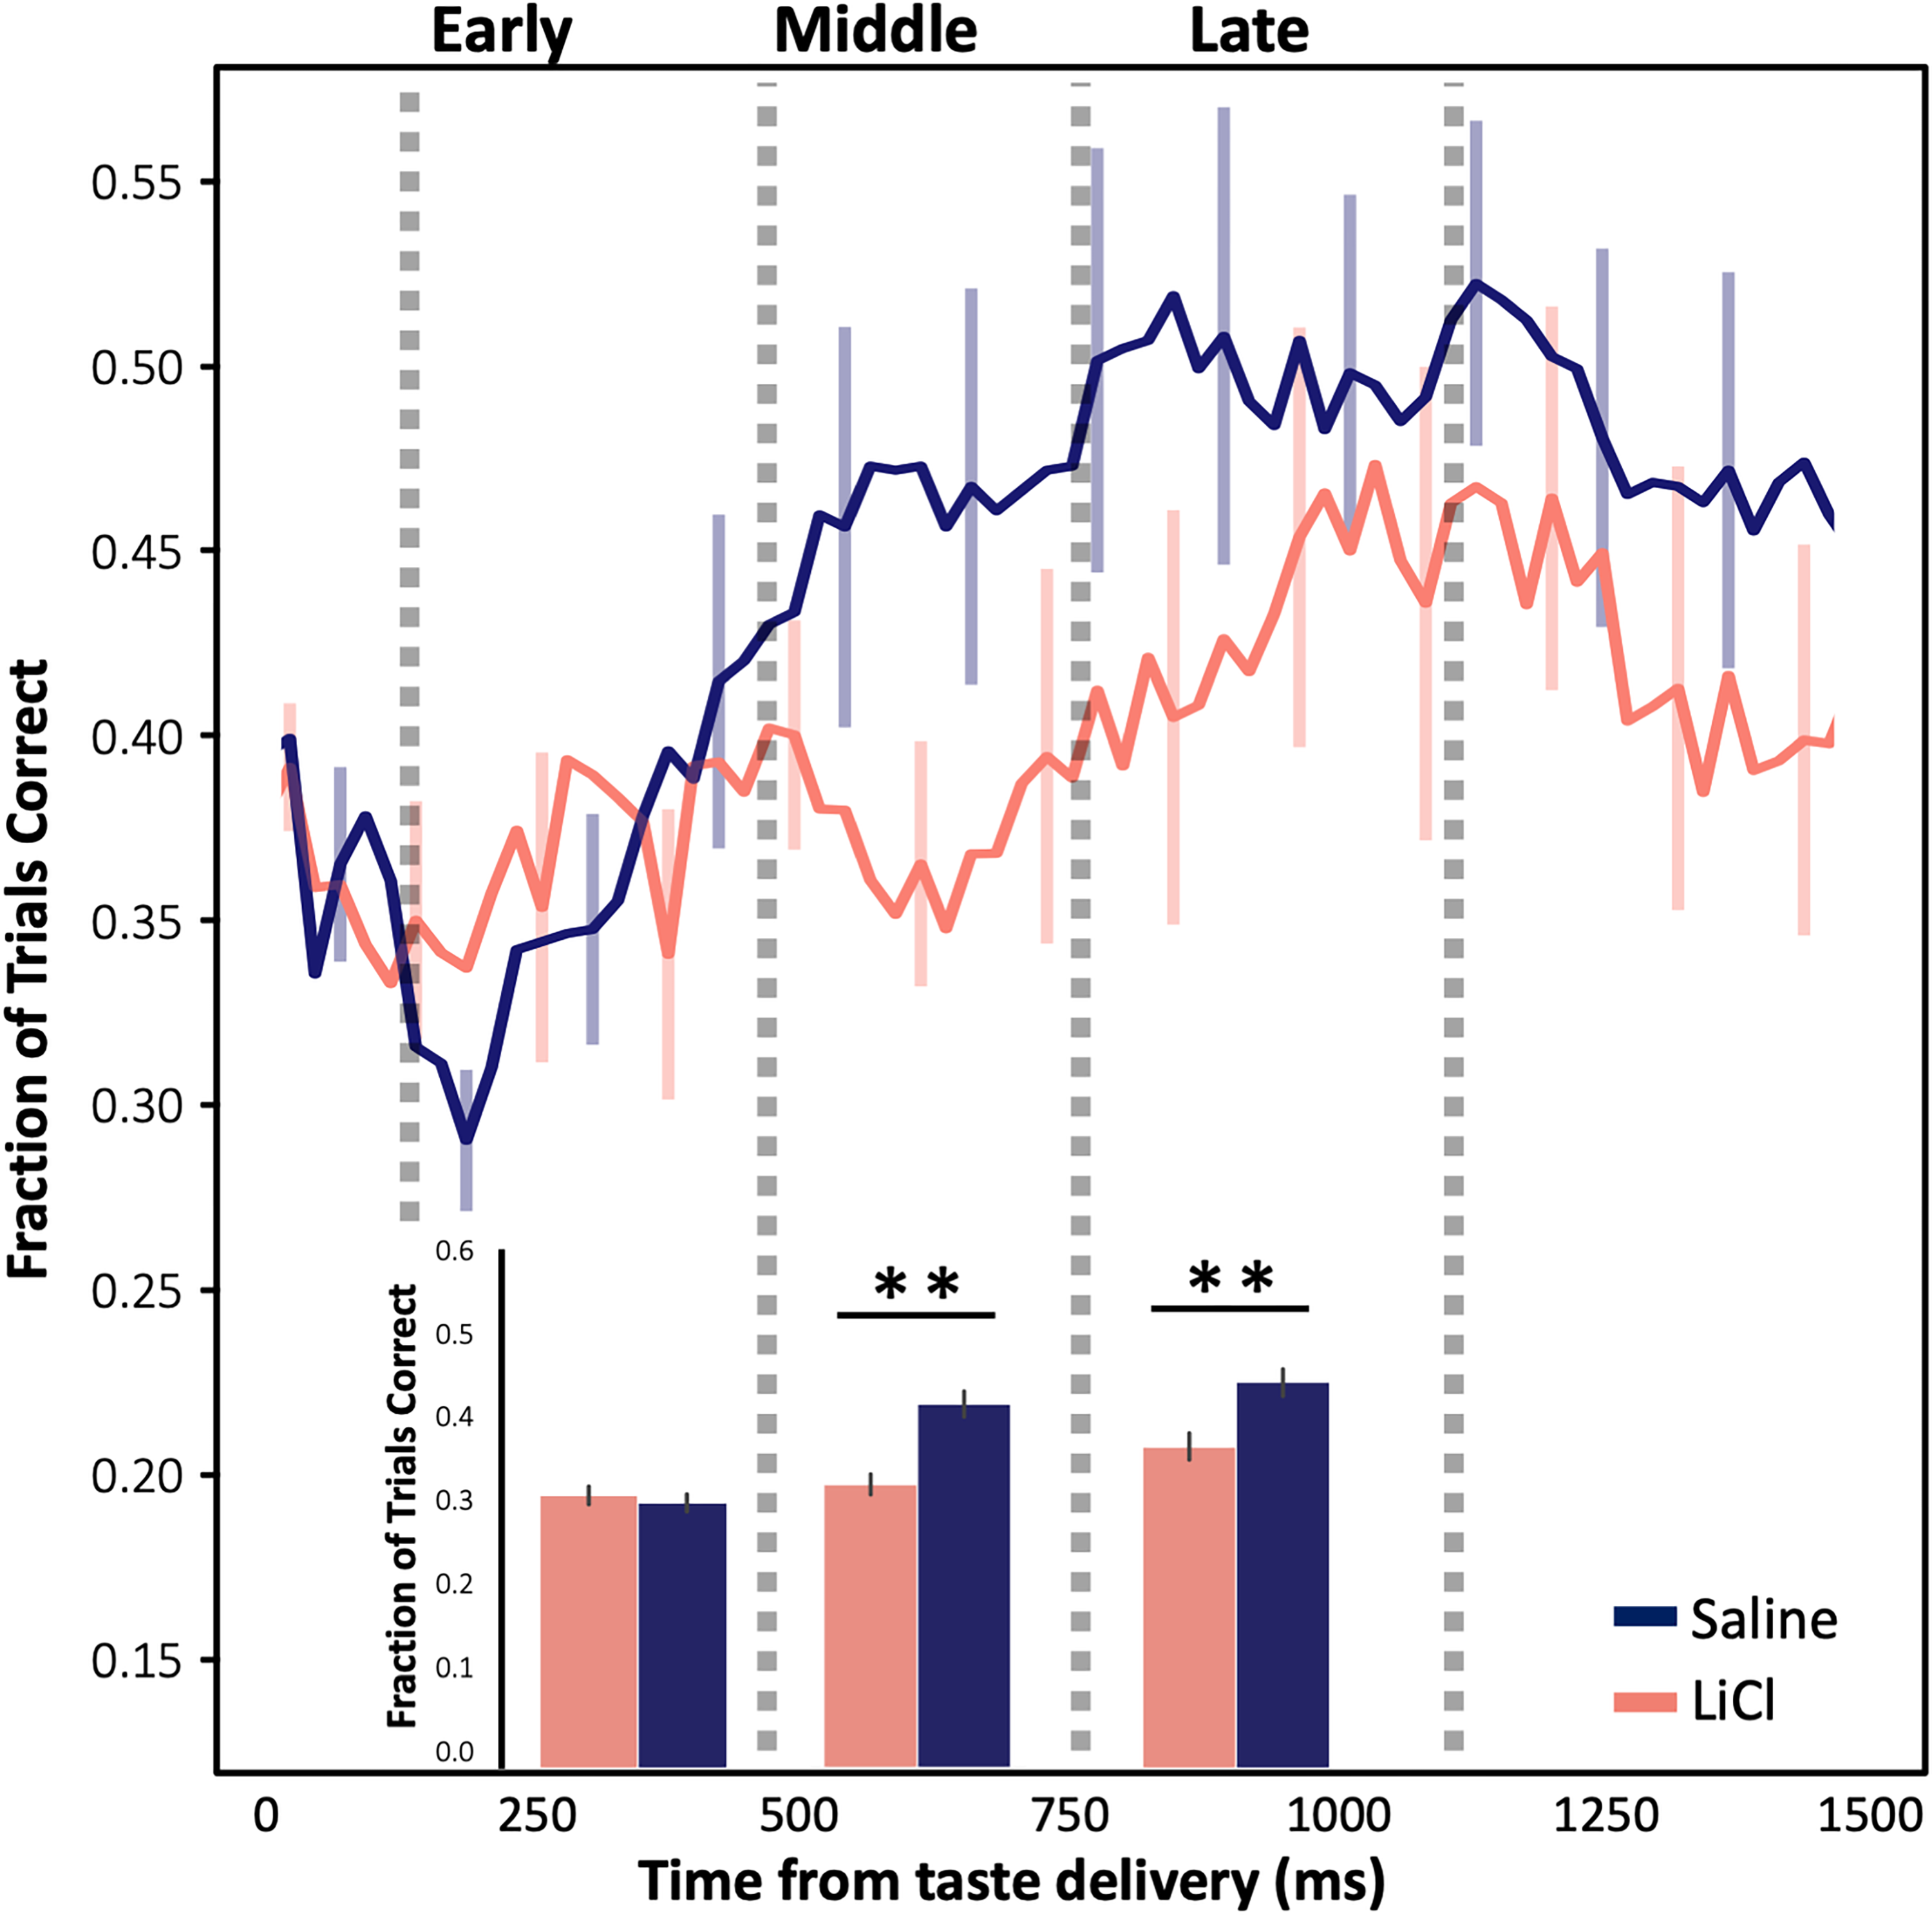
\includegraphics[width=\linewidth]{stone_2022_figs/journal.pbio.3001537.g005.png} 
\caption{\textbf{LiCl administration reduces taste discriminability in neural ensembles.} The time course of trials in which the taste could be correctly identified by ensemble firing, according to LDA, shows reduced discriminability of responses when an animal is sick (LiCl; coral, n = 174) in comparison to when they are healthy (saline; purple, n = 136). The vertical dashed lines delineate approximate epochal boundaries, as defined in previous research; collapsed into these epochs (bottom bars, the effect of illness only becomes significant within the middle (400–700 ms) and late (800–1,100 ms) epochs post taste delivery (** p \textless 0.01; pairwise t test with Bonferroni correction). The error bars represent SEMs. LDA, linear discriminant analysis; LiCl, lithium chloride.
}
\label{fig:wrapfig}
\end{figure}


The fact that this decrement in discriminability extends into the “late” epoch led us to ask whether LiCl-induced illness might also change the palatability-relatedness of coding as well (a feature that is known to emerge at this point in GC taste responses; see \cite{katz-a,katz2001a}). We began with the simple hypothesis that reduced discriminability should imply reduced palatability-relatedness, testing this hypothesis in the standard manner (\cite{sadacca2016a,levitan2019a,li2016a,piette2012a})—i.e., calculating moving window correlations between firing rates and the known canonical palatability ranks of the administered taste stimuli.

As has been observed many times previously, palatability-related information in our GC taste responses climbed (regardless of condition) across the period leading into the late epoch (Fig 2.6A; note that we currently have no explanation for the small, low magnitude, but significant saline-LiCl session difference in palatability-related firing in the earliest responses, but see Discussion); despite the well-known, oft-commented upon variability of sensory neural activity (\cite{shadlen1998a,shadlen1994a}), this property of GC taste responses shines through reliably in assessments of large numbers of neurons and across multiple animals. The climb calculated following saline and LiCl injections diverged significantly; however, particularly as the late epoch was reached—peak correlations following LiCl injections were higher than those observed in saline condition within this epoch (H(1) = 8.68, p = 0.003). This means that our initial hypothesis was disconfirmed: Whereas illness reduces taste response discriminability, it increases late epoch taste response palatability-related content.

\begin{figure}
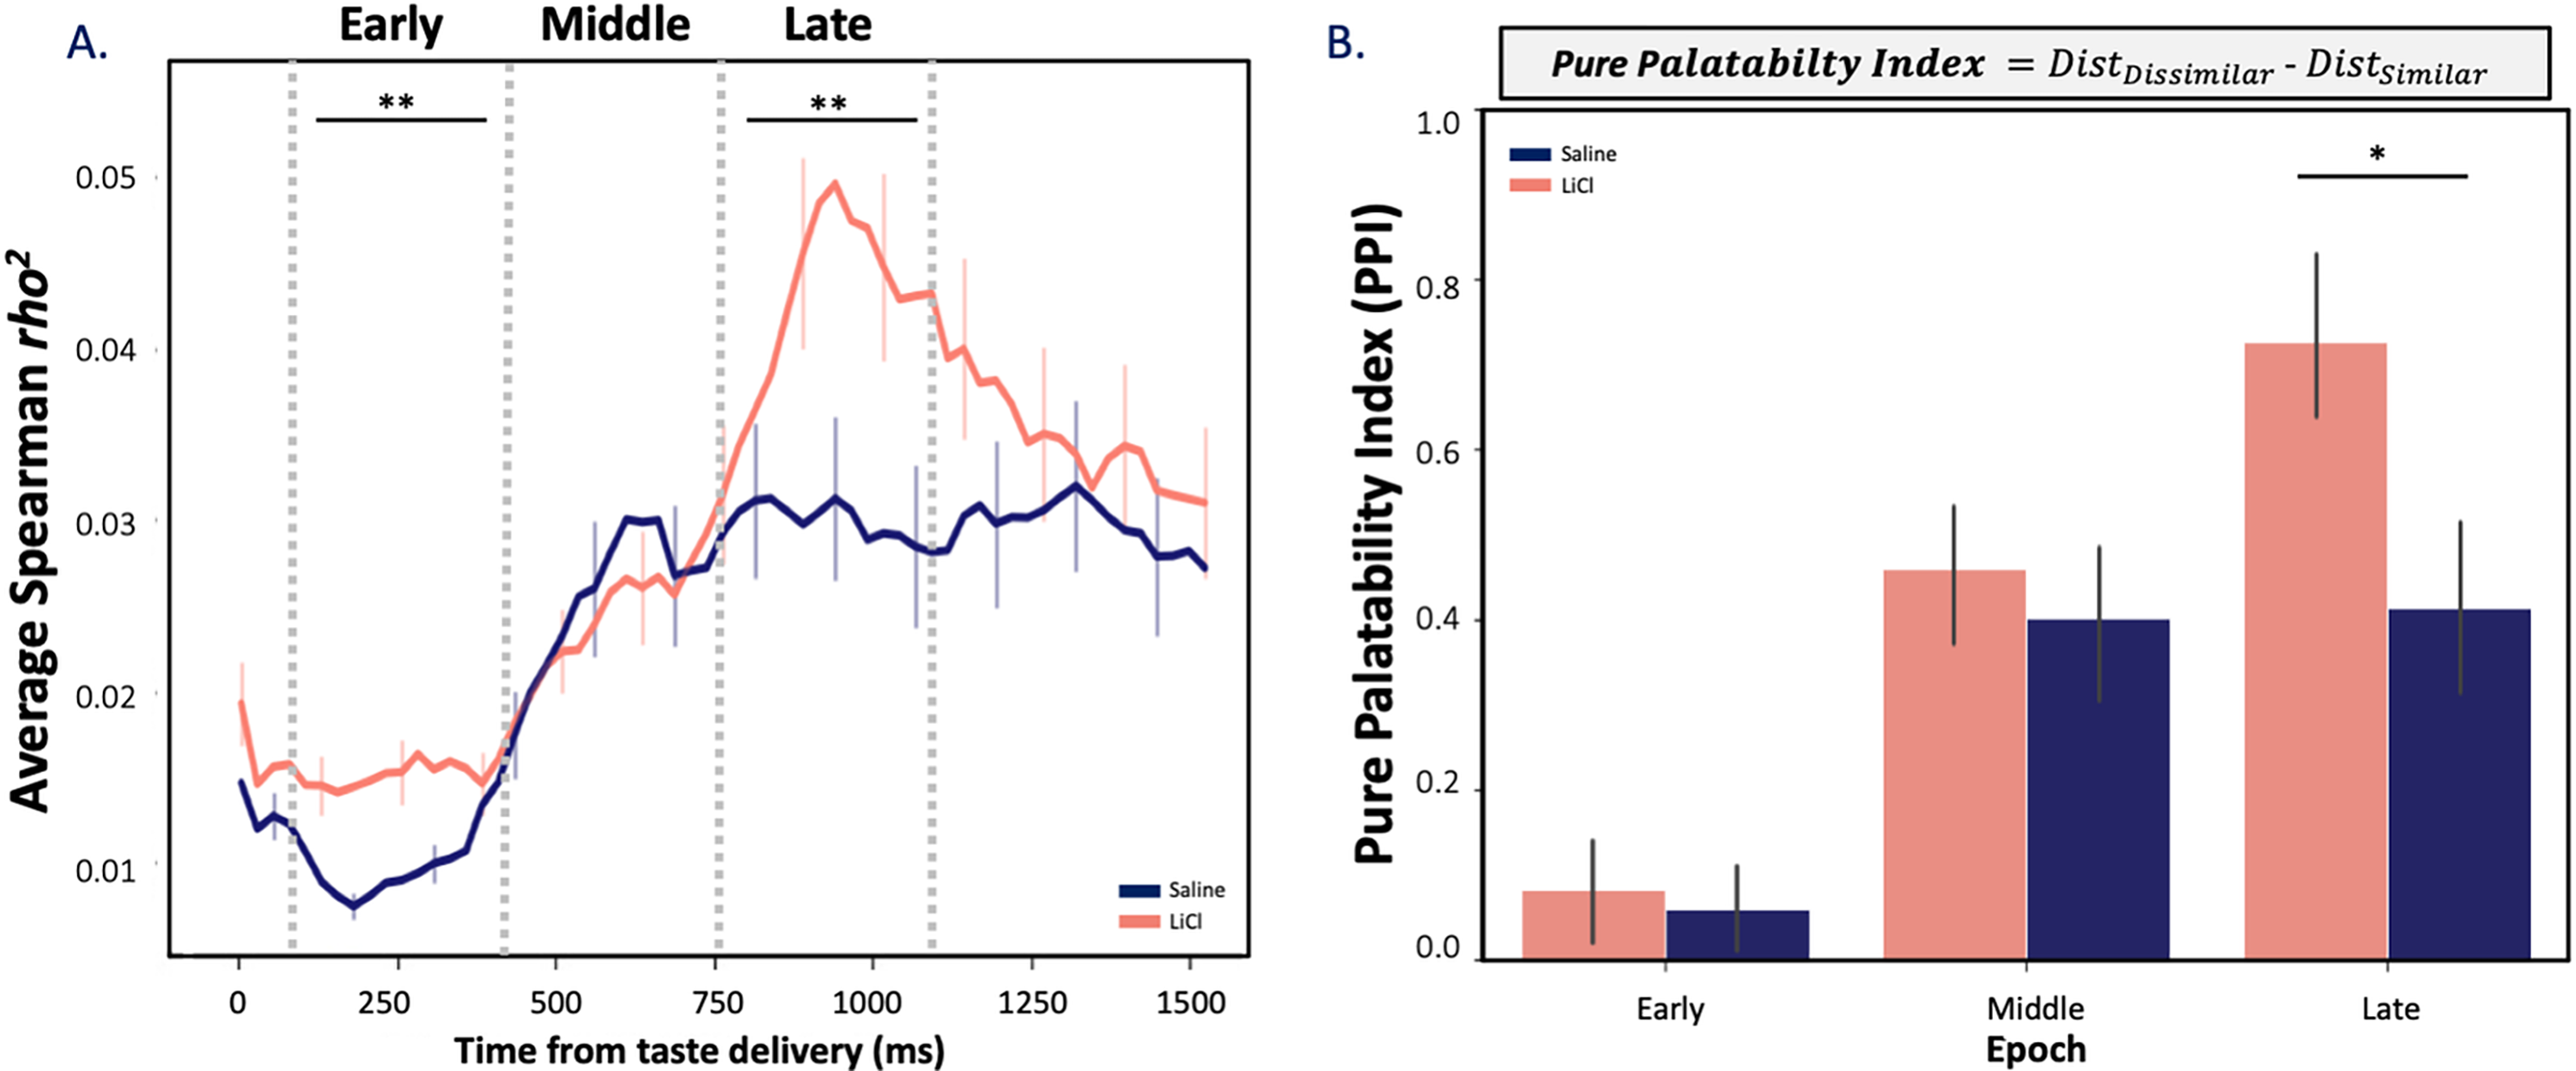
\includegraphics[width=\linewidth]{stone_2022_figs/journal.pbio.3001537.g006.png} 
\caption{\textbf{LiCl administration shifts GC taste responses in the direction of a simple “good vs. bad” judgment.}
\textbf{(A)} The time course of average correlations (Spearman rank-correlation coefficient) between firing rates and known palatability shows the expected increase as responses reached the late epoch, but this rise reached a higher peak following LiCl (n = 174) than saline injection (n = 136, Kruskal–Wallis H-test, ** p \textless 0.01). \textbf{(B)} The sickness-induced reduction of taste discriminability, juxtaposed with this sickness-induced enhancement of palatability-relatedness, suggests that illness selectively decreases the distinctiveness of tastes with similar palatability. As predicted, a PPI, which evaluates this possibility (see inlaid equation), peaks at a larger late epoch value following LiCl injection than following saline (unpaired 2-sample Wilcoxon test; * p \textless 0.05), reflecting sickness-induced polarization of coding. The error bars represent SEMs. GC, gustatory cortex; LiCl, lithium chloride; PPI, pure palatability index.
}
\label{fig:wrapfig}
\end{figure}


The above results beg the question “how can illness reduce information pertaining to identity while enhancing the palatability-relatedness of the same taste responses?” We hypothesized that these seemingly contradictory results could be reconciled if (and only if) illness causes GC coding to collapse toward a simple “good versus bad” judgment, preferentially decreasing the differences between the coding of tastes with similar palatabilities—making sucrose and NaCl (the palatable tastes) responses more similar and making quinine and citric acid (the aversive tastes) more similar—and leaving GC responses closer to a simplistic, “pure” code of whether or not a taste is palatable. We tested this hypothesis by quantifying the distance in Euclidean space between neural responses for all pairs of similar (e.g., sucrose and NaCl) and dissimilar (e.g., sucrose and quinine) taste stimuli.

Specifically, we calculated what we term a “pure palatability index”—the difference of the distances (DistDissimilar-DistSimilar) between responses to “different-palatability” and “same-palatability” tastes. By this analysis, the more polarized the response into “good versus bad”—the larger the difference—the more positive the PPI; a PPI of one (or greater) would indicate that GC neural responses are determined purely on the basis of whether the taste in question is pleasant or aversive. Fig 2.6B shows the results of this analysis. One-sample t tests comparing each PPI to a null result revealed that the PPI reaches significance only after the early epoch in both conditions (ps \textless 0.01); meanwhile, a Wilcoxon signed-rank test (performed because the data differed significantly from normal, p \textgreater0.05) revealed that LiCl-induced illness significantly enhances the PPI in the late epoch (W = 68379, Z = 0.54, p = 0.037, r = 0.09), reflecting enhanced polarization of the coding of palatable and aversive tastes. Thus, our second hypothesis was confirmed: Illness shapes the coding of taste hedonics by enhancing the polarization between similar and dissimilar tastes in the late epoch GC taste responses, and thereby simultaneously increases the overall palatability correlation and reduces the average discriminability of the responses.

\subsection{Illness-related changes in taste coding occur in single neurons}
The above results suggest that ensembles of GC neurons assayed approximately 20 min after LiCl administration code tastes differently than ensembles of GC neurons assayed in healthy rats. The implication of these results is that coding in individual neurons changes as sickness emerges, but the analyses above provide only indirect evidence for this implication; they stop short of directly testing whether single-neuron responses truly change with the onset of illness.

We therefore moved on to performing this direct test—2 such tests, in fact. First, we collected a new dataset using a modified experimental protocol in which we administered (and acquired spiking responses for n = 74 GC neurons to) tastes starting immediately after the injection of LiCl (Fig 2.7A). As already established, illness-related behaviors and changes in GC \(\mu\) power emerge by 20 min after LiCl injection (Figs 2.2 and 2.3); we therefore hypothesized that the above-described coding changes would emerge within single ensembles at approximately this same time point—that coding in trials delivered before sickness onset (“Pre”) would differ from that in trials delivered after sickness onset (“Post”; Fig 2.7A).

\begin{figure}
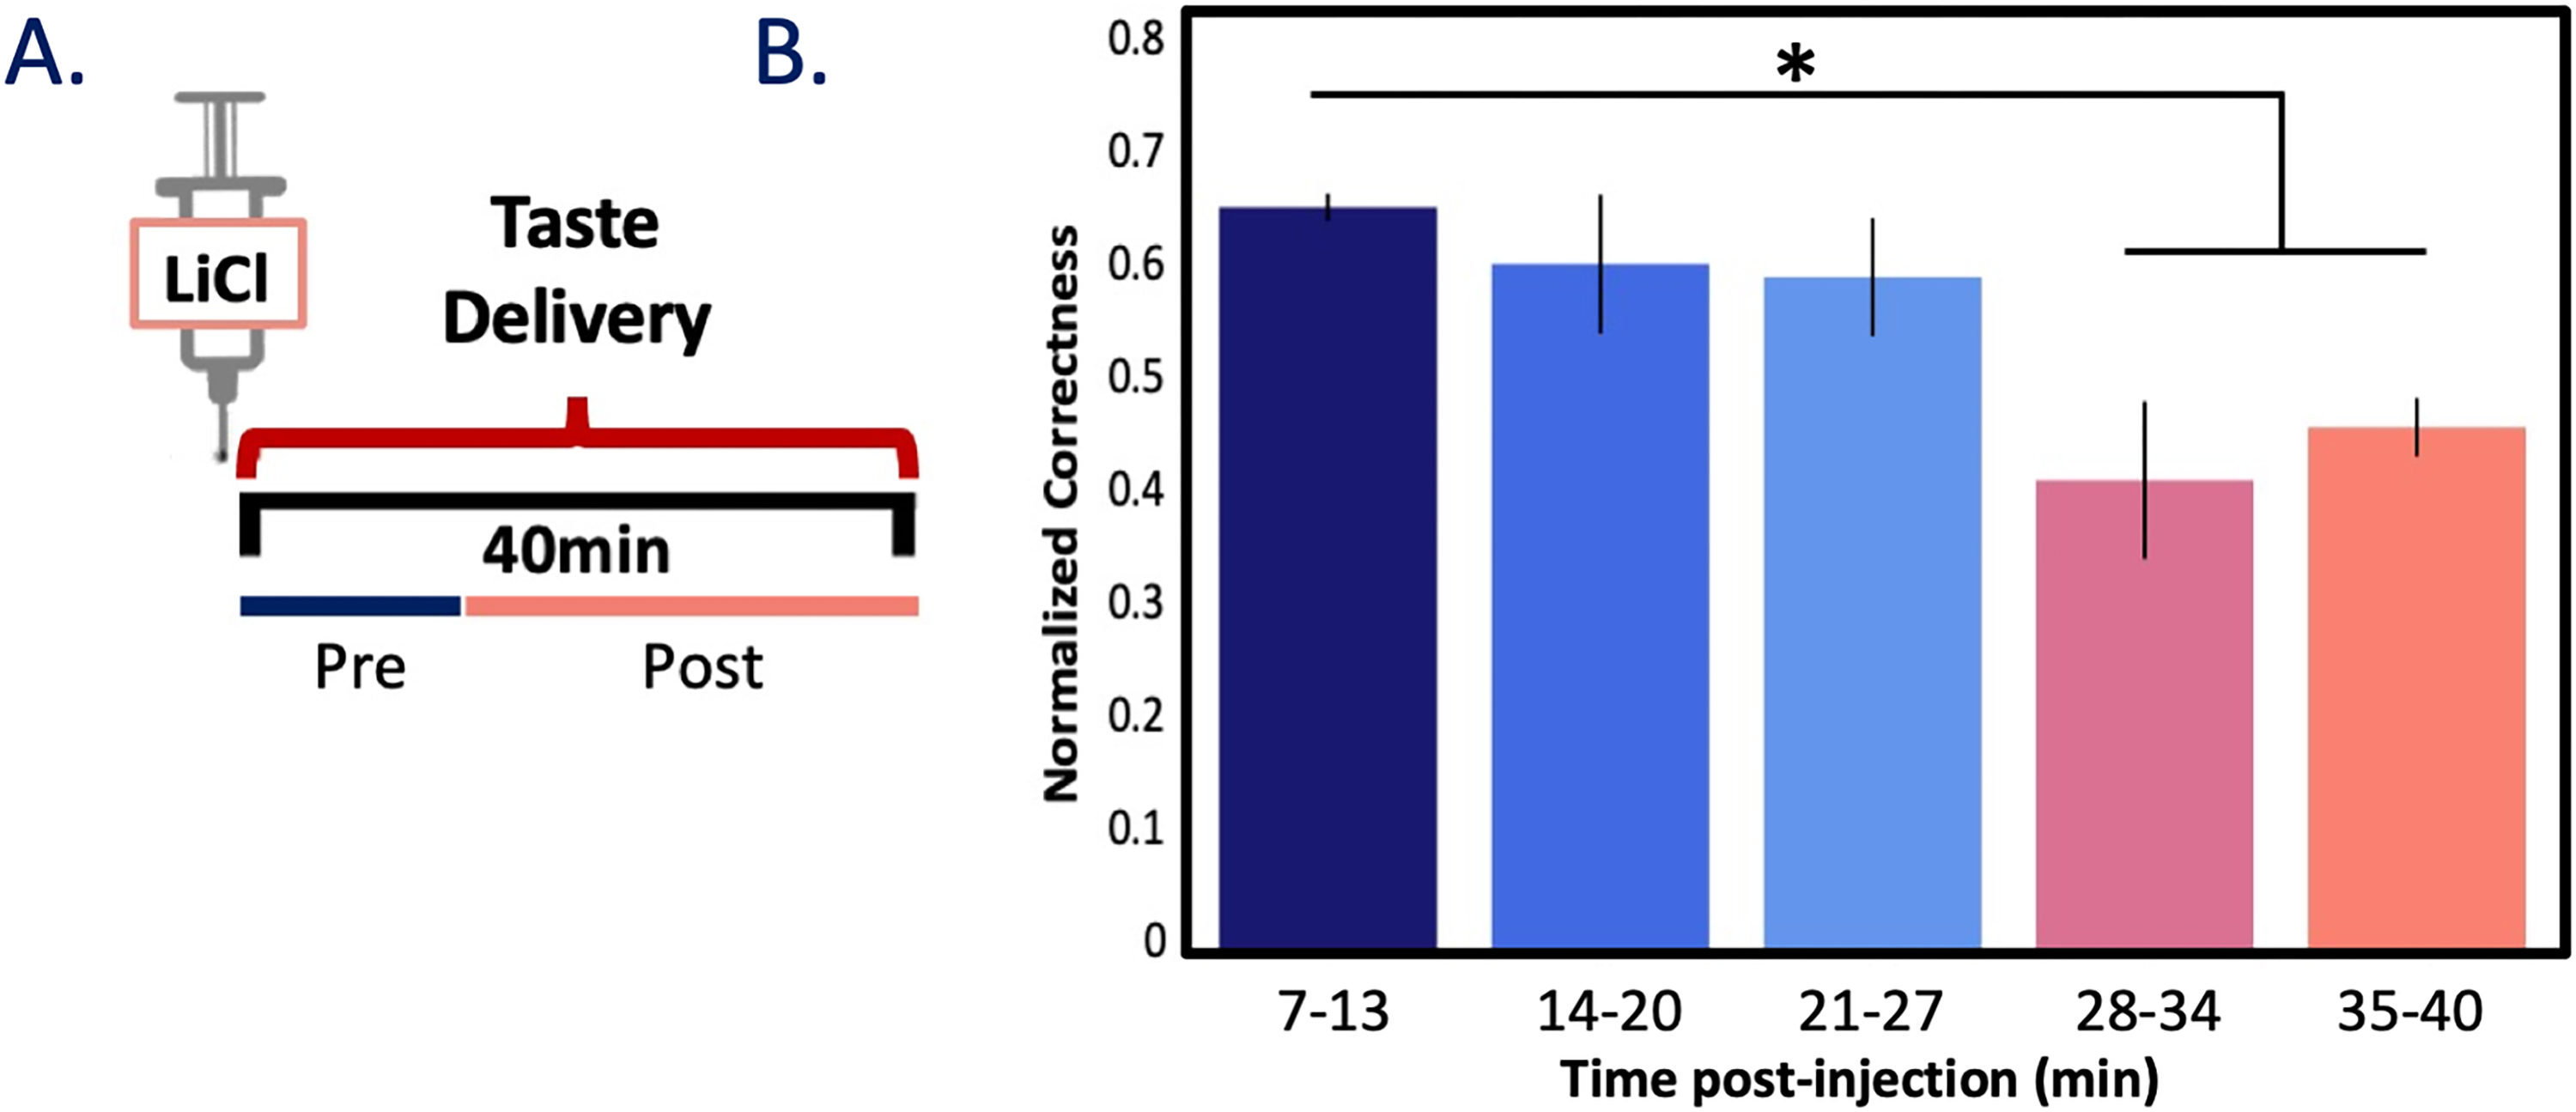
\includegraphics[width=\linewidth]{stone_2022_figs/journal.pbio.3001537.g007.png} 
\caption{\textbf{Reduction in taste discriminability emerges with sickness within session.} \textbf{(A)} A schematic of the second testing protocol, in which an injection of 0.15 M LiCl was immediately followed by delivery of tastants via IOC for approximately 40 min. \textbf{(B)} Bar plot shows the percent of trials in which the proffered taste was correctly identified using an LDA (trained on the first 5 trials) from GC responses. Across N = 3 animals (n = 56 taste responsive neurons), taste discrimination is significantly reduced post-sickness induction. * p \textless 0.05; paired t test with Bonferroni correction. The error bars represent SEMs. GC, gustatory cortex; IOC, intraoral cannulae; LDA, linear discriminant analysis; LiCl, lithium chloride.
}
\label{fig:wrapfig}
\end{figure}


We again used LDA to test whether and when taste response coding changed by testing the similarity of the first 5 “healthy” trials of each tastant to each subsequent taste delivery (binned; 5 trials/taste/bin). As expected, a repeated measures ANOVA performed between bins (bin = 6 min, approximately 3 trials/min) on taste responsive neurons (n = 56) revealed that the classifiability of tastes decreased significantly as rats became ill (F(4, 8) = 5.42, p = 0.02, np2 = 0.64), with this disruption becoming significant approximately 30 min into the session (Fig 2.7B, ps \textless 0.05). This result is a fairly good match for the above-described changes in GC \(\mu\) power and illness-related behaviors (Figs 2.2 and 2.3), particularly given the necessarily small sample of trials. While one could speculate that this effect is driven simply by time (as opposed to illness), this explanation is rendered unlikely by previous results demonstrating that, in the absence of illness, within-session taste discriminability does not vary significantly across much longer time spans (\cite{fontanini2006a}). The far more likely explanation is that taste responses change following the onset of illness.

We went on to more closely examine the precise nature of these changes in the subsample of our recorded neurons that were held across sessions—neurons in which we were able to assay responses after both LiCl and saline injections (see Methods for criteria). For each of 44 held neurons, we first examined session-specific firing rates for the 500 ms before and after taste delivery (starting after the initial 200 ms, which, as expected, was shown to be devoid of taste information in paired t tests). Visual examination of the data suggests that pre-stimulus firing rates in these neurons were not affected by LiCl administration (note that the small dots, which plot pre-stimulus firing, form a cloud going up the diagonal of Fig 2.8A, which plots the data for 1 representative taste [CA]). A paired t test confirmed that the mean pre-stimulus activity did not differ between saline (M = 6.68, SD = 4.71) and LiCl (M = 5.46, SD = 5.02) sessions (t(43) = 1.46, p = 0.15), and a Kolmogorov–Smirnov test confirmed the lack of a condition-specific impact on baseline firing rates (D(44) = 0.045, p = 0.98; Fig 2.8B), revealing that saline-LiCl difference in pre-stimulus firing rates were normally distributed and centered around 0.

\begin{figure}
\centering
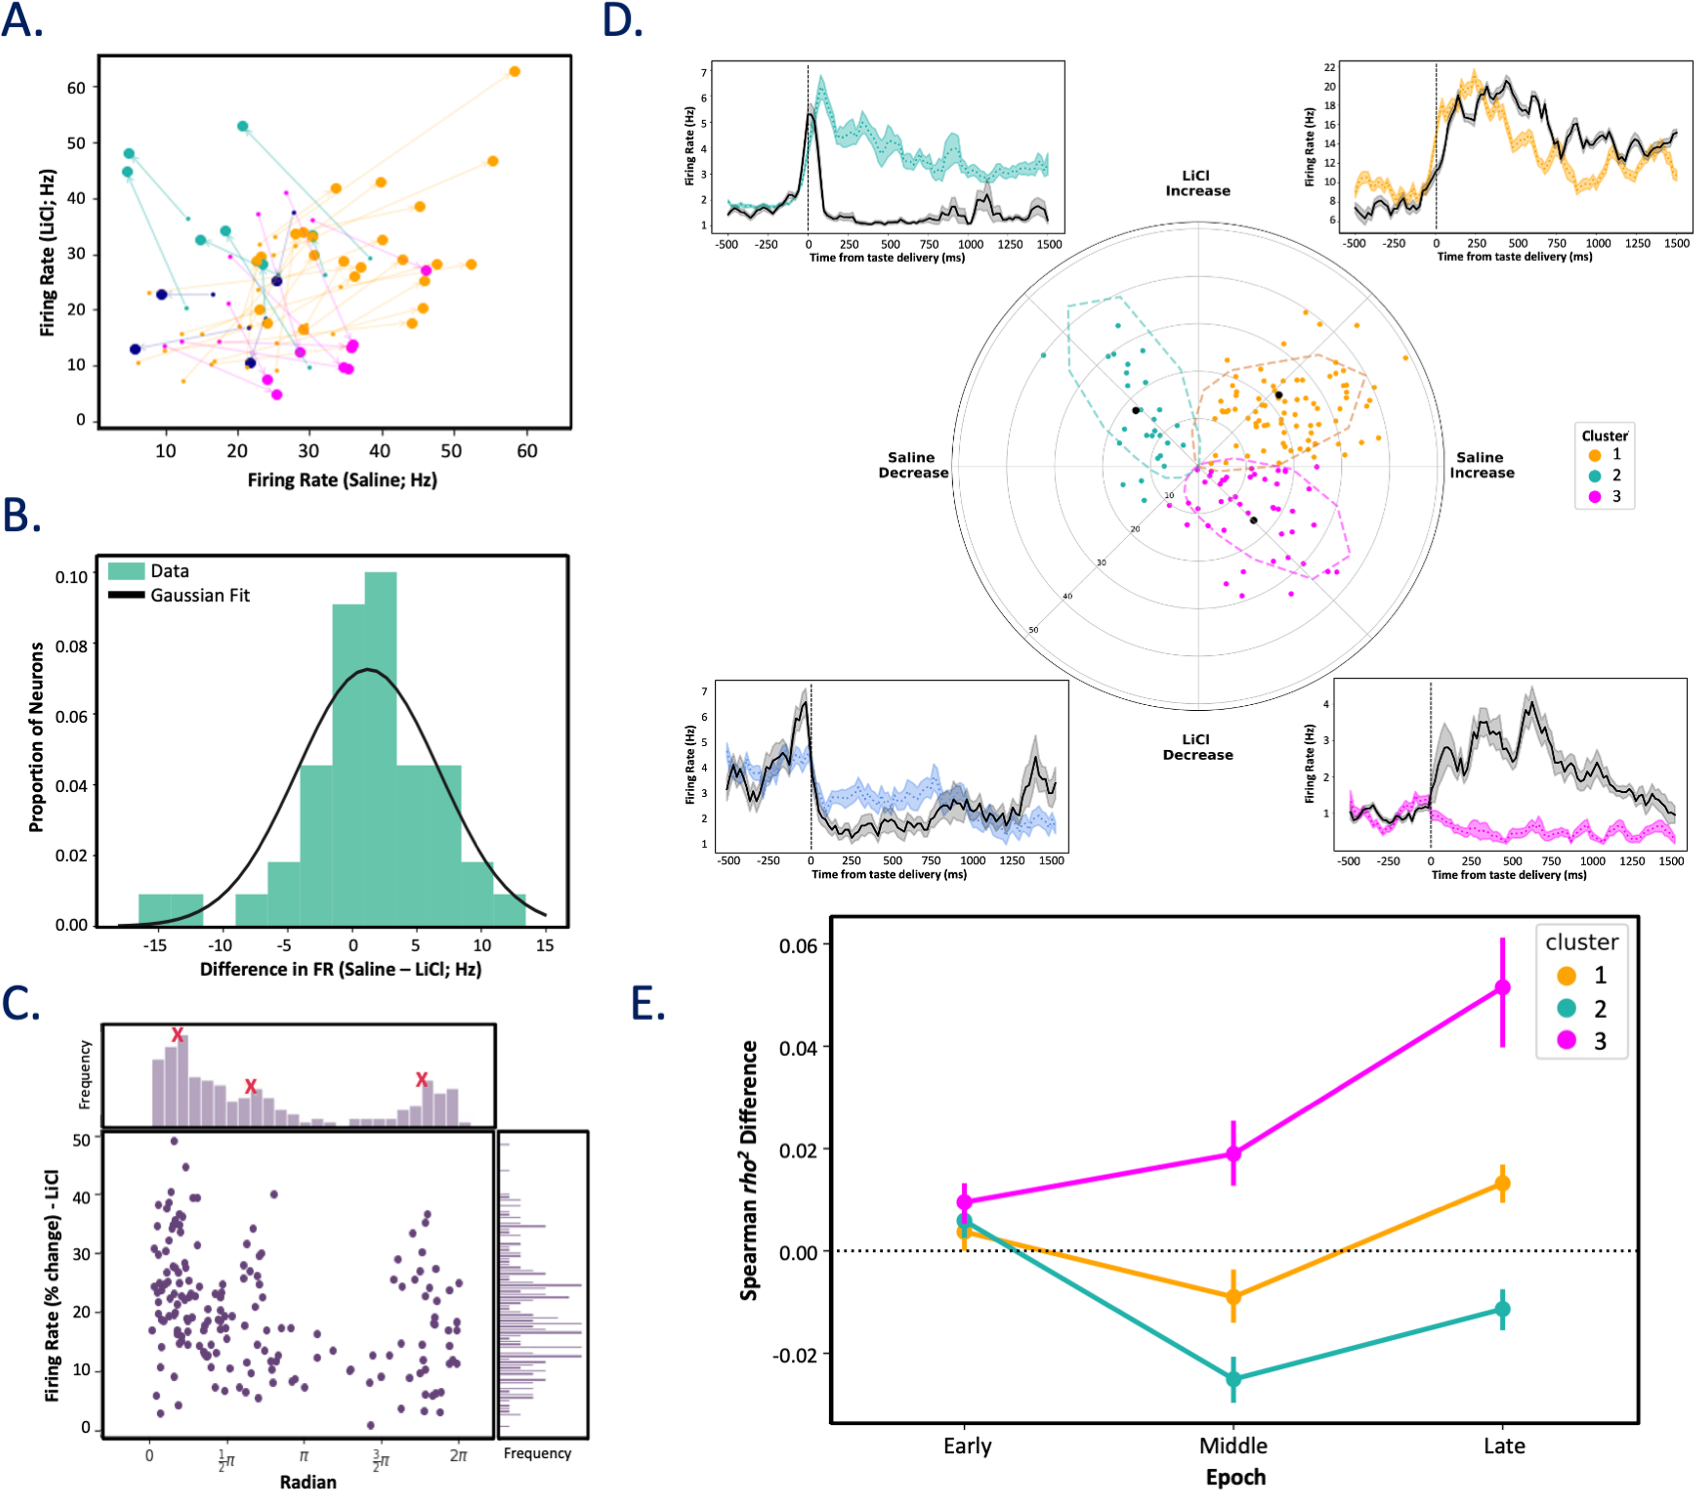
\includegraphics[width=0.8\linewidth]{stone_2022_figs/journal.pbio.3001537.g008.png} 
\caption{\textbf{Neurons held across post-LiCl and post-saline tasting sessions produce distinct clusters of taste response profiles.} \textbf{(A)} Firing rate trajectories for single neurons before (small circles) and after (large circles) taste delivery to the presentation of citric acid reveal condition-specific (sickness–y-axis, healthy–x-axis) taste response properties. Responses are colored with respect to angle of the response trajectory (0-90°, 90-180°, 180-270°, and 270-360° are yellow, teal, magenta, and blue, respectively), which highlights the distinct natures (excitatory, inhibitory) of responses in each condition. \textbf{(B)} A comparison of pre-stimulus activity suggests that post-injection firing rates did not differ between conditions: The peak of the distribution of saline-LiCl differences hovers around 0, and the distribution is fit well by a Gaussian (Kolmogorov–Smirnov test; p = 0.98); these facts suggest 0 difference (plus random noise). \textbf{(C)} A population response histogram (n = 44) held neurons depicting each neuron’s taste response (change from pre taste) as a function of vector direction in panel B confirms the presence of 3 unique peaks of vector direction (peaks indicated with red Xs). \textbf{(D)} A GMM was used to cluster cells based on response magnitude and trajectory. This analysis confirmed distinct cluster responses, revealed here in a polar plot (dashed lines denote 95\% confidence interval of cluster classification with respect to black-filled centroids). PSTHs for representative neurons are seen adjacent to the detected clusters, indicating taste responses post-saline (black) and post-LiCl (colored, cluster specific). \textbf{(E)} Cluster 3 (magenta) neurons reliably and selectively experience a sickness-induced increase in palatability-relatedness in the late epoch (nonparametric 2-way repeated-measure ANOVA; *** p \(<\)0.001). Vertical lines represent SEMs. GMM, Gaussian mixture model; LiCl, lithium chloride; PSTH, peristimulus time histogram.
}
\label{fig:wrapfig}
\end{figure}

Further scrutiny of Fig 2.8A, meanwhile, suggests 3 distinct “types” of impact. Cluster analyses confirmed these appearances, revealing 3 distinct and discrete clusters of taste-response changes wrought by sickness (identified with distinct colors attached to neurons in each cluster): (1) in some neurons, taste responses were excitatory in saline sessions but inhibitory during LiCl sessions; (2) in others, the reverse was true; and (3) in a third group of neurons, responses were excitatory in both states, but these excitatory responses were generally less strong following LiCl injections. Ancillary analysis confirmed the presence of these clusters in the full dataset, showing 3 peaks in the angle of the Fig 2.8A vectors (Fig 2.8C and 2.8D, the latter with representative examples of each type, as well as of the few neurons that fail to cluster).

These 3 clusters of neurons, which were sorted without regard to the types of information within the taste response, nonetheless differed with regard to how illness-inducing LiCl impacted palatability-relatedness in the dynamics of the taste responses. A 3-way nonparametric mixed ANOVA run on the palatability content of all neurons represented in Fig 2.8D revealed a significant interaction between cluster, epoch, and condition, F(4, 478) = 4.80, p = 0.001, indicating that the relationship between cluster (whether the neurons were in cluster 1, 2, or 3) and the coding of palatability within epoch was significantly different across the saline and LiCl conditions. Specifically, the late epoch enhancement of palatability-related firing described earlier proved to be primarily a function of one group of neurons—those for which normally excitatory responses were turned into inhibitory responses by LiCl-induced illness (F(1, 130) = 33.47, p = 5.12 × 10-8; Fig 2.8E). This result both confirms the validity of the separation of neuron types and reveals that this separation is related to the impact of illness state on palatability processing.


\section{Discussion}
Nutritional requirements, environmental conditions, and experience work together to guide consummatory behavior (\cite{parker1982a,provenza1995a,flores2018a}), in cooperation with an animal’s internal state (e.g., hunger, illness) (\cite{livneh2020a}). The study of how physiological states impact perception is an important one, because this relationship intrinsically controls the animal’s likelihood of survival. The fact that neurons are embedded in networks, and that the states of such networks can be indexed in terms of EEG power (particularly in \(\theta\) and \(\mu\) frequency ranges; \cite{fontanini2005a,fontanini2006a,fontanini2008a}), motivated our decision to characterize changes in LFP activity within GC as an animal shifts from a healthy state into one of emesis, and to then relate this shift to changes in the dynamics of taste coding. This analysis reveals a modulation of \(\mu\) power occurring approximately 15 min after LiCl injection—a result consistent with human (\cite{chen2010a}) and rat data (\cite{aguilar-rivera2020a}).

The finding that rearing durations, a measure of healthy exploratory behavior (\cite{parker1982a,tomasiewicz2006a,l2019a,aguilar-rivera2020a,alves2005a,rosana2012a}), drop at approximately the same time is consistent with decades of work showing that poisoning-related behaviors, and specifically those brought on by systemic nausea, emerge (depending on dose) at roughly 10 to 15 min post administration (\cite{parker1982a,nachman1963a,nachman1973a,aguilar-rivera2020a}). In our hands, the emergence of this LiCl-induced behavioral change closely mirrors the change in GC \(\mu\) power induced by the same LiCl dose, implicating the process whereby an animal experiences illness in generation of these neural changes.

Of course, the comparable timing of GC LFP activity and the emergence of sickness (as indicated by behavioral changes) cannot exclude the possibility that changes in GC activity could conceivably reflect, not illness per se, but rather a direct effect of LiCl on GC neurons. While unlikely, this alternative explanation would persist as a possibility even if we had shown illness-related behaviors and GC changes in the same rats (we used separate groups because the intentional subtlety of the illness-related rearing changes, which allowed us to avoid the possibility of GC changes reflecting massive changes in oral fluid handling, cannot be observed in rats attached to the electrophysiology/IOC harness). To completely disapprove this hypothesis, an additional set of experiments would be required, in which we somehow block every pathway whereby visceral inputs carry information regarding LiCl-induced gastrointestinal distress and test whether this manipulation also blocks cortical changes. In the absence of the huge expenditure of time and resources required for these experiments, the best solution involved testing a particularly rigorous and risky prediction: Rather than just predicting that LiCl would change cortical activity, we specifically predicted that LiCl would change cortical activity at about the same latency that it caused illness (measured in rearing behavior). Given the success of this prediction (see Figs 2.2, 2.3, and 2.7), the most likely explanation (by far) is that the 2 are linked—that LiCl-induced illness is reflected in cortical activity.

The change in GC \(\mu\) power is phasic, meaning that it is not simply the case that health connotes one \(\mu\) amplitude and illness a different \(\mu\) amplitude. This concept is not novel—while body states can be indexed in terms of LFP power fluctuations, behavioral states (e.g., sleep/wake) and muscle movements do not always correspond with a particular amplitude of field potential discharge (\cite{aston-jones1981a}) nor do significant changes in LFP power necessarily imply an observable change in body states (\cite{rojas-l2014a}). Like many dynamical systems, the cortex experiences transient periods of instability at the time of state changes; we postulate that the observed transient impact of LiCl administration on GC \(\mu\) power signals the onset of an illness state, and that the relaxation to a lower power regime shortly (approximately 7 min) thereafter nonetheless leaves the network changed in a way that impacts the processing of internal and external stimuli. In this, GC is akin to an automobile engine: Shifting from one gear to the next requires a brief transition from a steady state to a transient and then back to a steady state for optimal efficiency (\cite{oglieve2017a,horn2006a}).

In addition to altering \(\mu\) power, LiCl also significantly altered GC taste responses. This fact dovetails nicely with data presented by Arieli and colleagues (\cite{arieli2022a}), who examined how GC activity changes following CTA learning, identifying 2 types of impact resulting from the pairing of taste with LiCl-induced illness—an “immediate” impact of LiCl administration on taste responses in GC single neurons and a “delayed” impact on GC ensemble population dynamics in taste response. Arieli and colleagues hypothesized that the late impact is driven by CTA formation, and that the immediate impact is likely caused by the illness state induced by LiCl injection. Our current findings are consistent with theirs.

We went on to show that the impact of LiCl administration on taste coding is epoch dependent. The drug disrupted identity coding while (somewhat incongruously) enhancing the palatability-relatedness of the responses, with the latter effect localized to the oft-described late epoch of the responses (\cite{katz-a,katz2001a,sadacca2016a}). We also observed a small but significant illness-related increase in palatability coding in the early epoch. While an explanation for this unexpected result awaits further experimentation, we would speculate, based on work showing that expectation of stimulus availability can reduce that latency of gustatory coding (effectively eliminating the 200 ms non-chemosensory period observed in our work, see \cite{samuelsen2012a,gutierrez2010a,stapleton2006a,graham2014a,bouaichi2020a,dikecligil2020a}), that illness might similarly enhance the “readiness” of cortex and reduce the latency of taste-specific coding; since illness biases GC toward palatability-related coding (see below), it could very well be palatability coding that appears early when the animal is ill.

These findings may at first blush appear to be in conflict with previous studies examining behavioral changes following LiCl-induced illness; \cite{spector1988a,baird2005a,eckel1996a}, which suggested that sickness has no effect on palatability (e.g., as measured via evaluation of taste reactivity to a single taste (\cite{spector1988a})). In fact, however, our findings regarding sickness polarizing palatability processing are largely consistent with these results, in that they do not suggest wholesale changes in palatability of individual tastes, or even changes in the order of preference. Rather, we argue that illness simplifies taste coding, making aversive tastes more similarly aversive and palatable tastes more similarly palatable.

The results described in Figs 2.4–2.6 suggest, but do not prove, that single neurons change their coding as a function of illness. It is always possible that neurons coding taste identity and palatability during illness represent a distinct set of neurons from those coding these properties in healthy rats, and that the differences in overall sample responses reflected the addition of this new set of “illness-only” responses. In the first test of the hypothesis that illness changes the processing of taste stimuli in individual neural ensembles, we showed that taste discriminability is significantly changed as an animal enters the emetic state. And since the small number of trials available in this analysis rendered it impossible to reliably compare palatability correlations, we performed a second analysis in which we leveraged our ability to hold a subset of our single neurons across both testing sessions. This analysis revealed that LiCl-induced illness enhances palatability-relatedness in an epoch-specific manner but went beyond this to reveal 3 distinct subpopulations of illness-related response profiles.

We cannot, as of yet, provide a definitive explanation of this functional dissociation of GC neurons, but we can speculate as to several mechanisms that could explain our results. The most parsimonious of these explanations might be that the clusters come from either functionally or physiologically distinct populations of cells which in turn code specific features about the state of the animal (and thus responses to external stimuli) in unique, yet beneficial ways. However, cross-correlational analysis (methods adapted from \cite{li2013a}) failed to reveal differences in the strength of the functional connectivity between (nor within) the individual clusters, which would have been expected with such an explanation (\cite{li2013a}). Furthermore, analysis of wave shapes and basal firing rates failed to reveal groups to be made up of different percentages of putative pyramidal and interneurons. While it is always risky to reach conclusions on the basis of a null result, particularly in small datasets, we find it unlikely that these clusters represent distinct types of GC neurons.

An alternative explanation for the observed differences in palatability coding across these putative clusters has to do with the possible sources of input to these neurons. It has recently been shown that specific area postrema neuron types are responsible for providing illness-related information to brain regions (\cite{zhang2021a}), and that these influences may reach GC by way of either the nucleus of the solitary tract (\cite{shapiro1985a}) or other regions (e.g., amygdala) known to be impacted by the physiological state induced by LiCl (\cite{spencer2012a}). It is possible that the palatability-coding differences between GC clusters are a downstream result of cell type–specific projections. Future work will examine this possibility, incorporating the use of video recordings of oral-facial reactivity to establish the link more concretely between these putative clusters and their behavioral relevancy in consummatory behaviors.

Regardless of the answers to these questions, the work presented here demonstrates that illness, or at least that caused by LiCl, impacts cortical function in a far more refined manner than via a simple wholesale disruption of activity. The effects of illness on GC activity are complex, but this complexity seems linked to an animal’s need, when ill, to simply tell good from bad. In fact, this is not the first case we have found a manipulation that biased GC response toward stimulus palatability. \cite{fontanini2006a} also found that when the behavioral state of an animal changed from a task-oriented to a disengaged (or inattentive) state, GC response became less discriminative between palatability-similar tastes but more distinct for tastes with opposite valences. The similarity in impact of illness and engagement states provides further support for the general finding that GC is involved in the making and putting into action of decisions related to palatability (\cite{sadacca2016a,mukherjee2019a}): While the most basic circuit involved in these decisions is found in the brainstem (\cite{grill1978a,grill1978b,geran2006a}), the taste system is very much like other vertebrate and invertebrate sensorimotor systems (\cite{geran2006a})—in situ, top-down modulation plays a major role in determining behavior. Here, GC plays that role, and this is possibly why body states are reflected in GC as well.

\printbibliography[title={References}]

\end{refsection}
\begin{refsection}

\chapter[BLA-GC Dynamics]{Coupled dynamics of stimulus-evoked gustatory cortical and basolateral amygdalar activity}

\section{Abstract}
Gustatory cortical (GC) single-neuron taste responses reflect taste quality and palatability in successive epochs. Ensemble analyses reveal epoch-to-epoch firing rate changes in these responses to be sudden, coherent transitions. Such nonlinear dynamics suggest that GC is part of a recurrent network—that GC produces these dynamics in concert with other structures. basolateral amygdala (BLA), which is reciprocally connected to GC and central to hedonic processing, is a strong candidate partner for GC: BLA taste responses evolve on the same general “clock” as GC; furthermore, inhibition of activity in the BLA->GC pathway degrades the sharpness of GC transitions. These facts motivate, but do not test, our over-arching hypothesis that BLA and GC act as a single, co-modulated network during taste processing. Here we provide just this test of simultaneous (BLA and GC) extracellular taste responses in female rats, probing the multi-regional dynamics of activity in these regions to directly test whether BLA and GC responses contain coupled dynamics. We show that BLA and GC response magnitudes covary across trials and within single responses, and that changes in BLA-GC LFP phase-coherence are epoch-specific. Such classic coherence analyses, however, obscure the most salient facet of BLA-GC coupling: sudden transitions in and out of the epoch known to be involved in driving gaping behavior happen near-simultaneously in the two regions, despite huge trial-to-trial variability in transition latencies. This novel form of inter-regional coupling, which we show is easily replicated in model networks, suggests collective processing in a distributed neural network.

\section{Introduction}
As a rat feeds, gustatory cortical (GC) single-neuron taste responses take the form of a sequence of distinct “epochs” separated by sudden ensemble transitions. The epoch that starts at 0.5-1.5sec (depending on the trial) contains firing that is staunchly palatability-related; the transition into that epoch, which is so sudden that it is analytically indistinguishable from state switching (\cite{sadacca2016a} see below for distinction of the terms “epoch” and “state”), both predicts and drives taste-related oral behavior (\cite{sadacca2012a,li2016a,mukherjee2019a}). Theory suggests that such dynamics are most easily generated by a distributed circuit in which strong recurrent connectivity (\cite{maass2007a, miller2010a, miller2013a,edelman2013a,mante2013a,kietzmann2019a}) couples “separate” regions into a single processing unit; such recurrence is abundant within the taste circuit (\cite{bielavska1996a,mcdonald1998a,shi1998a}).

Particularly notable in this regard is the reciprocally-connected GC-basolateral amygdala (BLA) dyad. Work investigating these brain regions separately (\cite{katz2001a,fontanini2009a,sadacca2012a}) has revealed striking similarities in the trial-averaged dynamics of their taste responses. Furthermore, BLA-GC connectivity has proven important for both taste learning (\cite{lin2012a,lin2015a,lavi2018a,kayyal2019a}) and taste processing (\cite{lin2021a}). This latter study specifically demonstrated that the suddenness of the behaviorally-relevant GC ensemble transitions to the palatability epoch are degraded by inhibition of BLAGC axons. These results provide indirect evidence for a general hypothesis that BLA and GC work together during taste processing, but stop far short of testing the existence of dynamic BLA/GC coupling; in fact, there has been little work directly investigating communication between any pair of taste-relevant brain regions (but see Di Lorenzo and Monroe, 1997).

Work investigating pairs of regions involved in other processes—decision making (\cite{antzoulatos2016a,place2016a,zielinski2019a}), sensory-motor transformation (\cite{arce-mcshane2016a}), vision (\cite{bastos2015a,zandvakili2015a,saravani2019a,lundqvist2020a}), and motor planning (\cite{yates2017a,ames2019a})—has revealed inter-regional spiking and field potential coherence, but has done so using metrics for which temporal resolution, particularly at the single-trial level, is limited. Given the epochal nature of taste processing, the suddenness of GC ensemble transitions into palatability-responsiveness, and the trial-specific latency of this transition, testing GC-BLA coupling requires techniques that permit evaluation of the moment-to-moment evolution of the BLA-GC relationship. The fact that the suddenness of GC ensemble transitions (\cite{sadacca2016a,mukherjee2019a}) depends upon an intact BLA-GC pathway (\cite{lin2021a}) motivates our novel, central prediction: that this moment of transition will be coupled across BLA-GC ensembles. 

Here, we present an in-depth investigation of BLA-GC taste-response coordination, beginning with “canonical” methods (correlations of spiking in whole trials, and phase-coherence of local field potentials [LFP] across trials) and progressing to the testing of our novel hypothesis. The former allows us to show trial-specific and time-varying coupling in BLA and GC taste responses—reductions in phase-coherence (\cite{stitt2017a}) that appear and vanish in an epoch-specific manner. But since these analyses necessarily obscure coupling in the trial-specific timing of sudden state-to-state ensemble transitions, we move on to explicit modeling of state transitions in ensemble timeseries data (\cite{rabiner1989a,sadacca2016a}); these analyses allow us to confirm our prediction that BLA-GC coordination integrally involves sudden, brief coupling of the specific transitions that predict and drive palatability-related behavior. Finally, computational modeling demonstrates that these results (coordinated state transitions with variable state-wise functional connectivity) are easily recapitulated within a simple multi-region network. These results overall lead us to suggest that BLA and GC form a functional “unit” for purposes of taste processing. 

\section{Materials and Methods}


\textbf{Subjects}\par
\noindent Adult, female Long-Evans rats (n = 8; 300–350g at time of electrode implantation, Charles River Laboratories) served as subjects in our study (we have observed no sex differences in the basic cortical dynamics of taste responses between male and female rats, and therefore use female Long-Evans rats because they are, in our hands, calmer than males). The rats were housed in individual cages in a temperature- and humidity-controlled environment under a 12:12 hr light:dark cycle, given ad libitum access to food and water prior to the start of experimentation, and weighed daily following surgery to ensure that they never dropped below 80\% of their pre-surgery weight. All experimental methods were in compliance with National Institutes of Health guidelines and were approved in advance by the Brandeis University Institutional Animal Care and Use Committee.

\smallskip
\noindent\textbf{Electrode and intra-oral cannula construction}\par
\noindent Custom microwire bundle drives were made with either 16 or 32 electrodes per recording site (design and construction details available at https://katzlab.squarespace.com/technology). Intra-oral cannulae—flexible tubing with a flanged tip and washer to ensure stability, connected to a plastic top complete with a locking mechanism—were built to allow the delivery of tastants directly onto the tongue (Fontanini and Katz, 2006).

\smallskip
\noindent\textbf{Acquisition of electrophysiological data }\par
\noindent Electrophysiological signals from the micro-electrodes were sampled at 30 kHz using 32-channel analog-to-digital converter chips (RHD2132) from Intan Technologies, digitized online at the head stage and sampled jointly, along with signals from actuators marking tastant delivery, using an Intan RHD USB interface board (Part \#C3100), which routed records to the hard drive of a PC for saving. The experimental chamber was ensconced in a Faraday cage that shielded recordings from external electromagnetic influences.

\smallskip
\noindent\textbf{Surgery}\par
\noindent Rats were anaesthetized with an intraperitoneal injection of ketamine/xylazine cocktail (100mg/kg and 5.2 mg/kg respectively) and mounted in a stereotaxic instrument (David Kopf Instruments; Tujunga, CA) with blunt (atraumatic) ear bars. A midline incision exposed the skull and trephine holes (approx. 2 mm diameter) were drilled above BLA and GC. For 6 (out of 8) rats, microwire bundles were implanted 0.5mm above GC (coordinates: AP +1.4 mm, ML -5.0 mm, DV -4.4mm from dura) and BLA (coordinates : AP -3.0mm, ML -5.0mm, DV -6.8mm from dura). For the remaining 2 rats, bundles were instead implanted bilaterally above BLA. Once in place, electrode bundles were cemented to the skull. Once electrode bundles were secured, an intra-oral cannula (IOC) was threaded through the masseter muscle (inside the zygomatic arch) to the space between the lip and gums, and the top of the cannula was cemented to the rest of the assembly with dental acrylic (Fontanini and Katz, 2006). The rat’s body temperature was monitored and maintained at approx. 37°C by a heating pad throughout the duration of the surgery.

\smallskip
\noindent\textbf{Habituation and passive taste administration}\par
\noindent Following their recovery from surgery, we habituated rats to the experimental chamber for 2 days, to the IOC/electrode harness for the next 2 days, and to passive water deliveries for the following 2 days, before beginning data collection. Starting with the second habituation day, we also placed rats on a mild water restriction schedule—20mL of water (not including the approx. 4mL delivered during habituation sessions themselves) per day. This water restriction schedule was maintained till the end of the experiment. For the 2 final habituation sessions, we attached the rats to the taste delivery apparatus, and infused 120 pulses of distilled water (approx. 30\(\mu\)L per pulse; 20s inter-pulse interval) into the animal’s oral cavity through the IOC, and drove electrode bundles deeper (by 250 \(\mu\)m) into target structures. By the end of this procedure, the tips of the electrodes lay within GC and BLA. We then recorded taste responses during 3-4 days of taste delivery sessions, between each of which the microwire bundle was driven down approximately 60 \(\mu\)m. During these sessions, Sucrose (0.3M), Sodium Chloride (0.1M), Citric Acid (0.1M), and Quinine (1mM), dissolved in ultra-pure water (approx. 30\(\mu\)L per pulse; 20s inter-pulse interval, 30 trials/tastant) were delivered to passive rats (i.e., no behavior was required to elicit delivery). These concentrations were chosen to represent a range of hedonic values, and because they are known to evoke robust responses in both GC and BLA (\cite{fontanini2009a,sadacca2012a}).

\smallskip
\noindent\textbf{Histology}\par
\noindent In preparation for histology, rats were deeply anesthetized with an overdose of the ketamine/xylazine mixture. We perfused the rats through the heart with 0.9\% saline followed by 10\% formalin and harvested the brain. The brain tissue was incubated in a fixing mixture of 30\% sucrose and 10\% formalin for 7 days before being sectioned into 50\(\mu\)m coronal slices on a sliding microtome (Leica SM2010R, Leica Microsystems). Sections containing the electrode implant sites around GC and BLA were imaged at 2x.

\smallskip
\noindent\textbf{Data and statistical analyses}\par
\noindent The analysis of data and statistical tests were performed using custom written software in Python and MATLAB (The MathWorks, R2018a), as described below.
Local Field Potential processing and analysis

\smallskip
\noindent\textbf{LFP Analyses}\par

\noindent\underline{Filtering / power and phase extractions}
LFPs were extracted from broadband digitized signals using a 2nd order bandpass Butterworth filter (1-300Hz), to de-emphasize spiking and emphasize frequencies typically of interest in such data. In order to avoid contamination from noise/artifacts on noisy/broken channels, only channels containing isolable single neurons (see below) were used for analyses. Estimates of instantaneous power and phase in delta (1-4Hz), theta (4-7Hz), mu (8-12Hz), beta (12-30Hz), gamma (30-100Hz) bands were extracting using the Short Time Fourier Transform (STFT) implementation in Scipy (\cite{p2020a}) with a 500ms window and 99\% window overlap.

\smallskip
\noindent\underline{LFP Phase Coherence}
Phase coherence analysis was performed, as per Kramer and Eden (2020), to provide a basic, dynamic, trial-averaged evaluation coupling of BLA and GC as visible in LFPs. We selected for this analysis the electrodes from which activity was most similar to the mean activity for the region (smallest mean-squared error relative to the mean phase across all channels for each region; this selection of channels was constant for all trials in a single analyzed session, and the same set of channels was used for all frequencies), to ensure reliable representation of each. The difference in phase between the (GC and BLA) pair of electrodes for each timepoint was calculated across all trials, and the mean of those phase-difference vectors was calculated for each timepoint, the magnitude of which represents the coherence strength.  Coherence values were averaged across small canonically-defined frequency bands: theta (4-7Hz) and mu(8-12Hz). Results in other bands were comparable (see Results). The specific calculation was as follows:

$$\text{Coherence}_{\text{GC}\leftrightarrow\text{BLA}}(f)=\abs{\frac{1}{N}\sum_{n=1}^{N}e^{-i(\theta_t^\text{GC}(f)-\theta_t^\text{BLA}(f)}}$$
\noindent Where \(\theta_t^\text{GC}(f)\) and \(\theta_t^\text{BLA}(f)\) are the GC and BLA LFP phases for time “t” and frequency “f”, and “n” is the counter for number of trials.

\noindent The error term for the evaluation of coherence magnitude was estimated using bootstrapping, by resampling trials with replacement from individual recordings (500 such resamples were performed for each recording). Changes in taste-induced coherence were determined relative to baseline (the 750 to 250ms period prior to stimulus delivery was selected as baseline, with timepoints closer to stimulus delivery ignored to avoid temporal “bleed” of coherence between pre- and post-stimulus periods due the slow frequencies considered here); if the mean value of the coherence during taste responses fell outside the 95\% CI of the baseline period (see above), the deviation was deemed significant. The fraction of recordings with significant deviations were summed at each timepoint and across all recordings, enabling an estimation of the aggregate dynamics of these changes, and the resultant time-series were smoothed (to remove brief, spurious deflections) using a 2nd order Savitzky-Golay filter with a 101 ms kernel (Press and Teukolsky, 1990). To visualize the dynamics of this phase coherence, changes in coherence from baseline were calculated for 4-7, 7-12, 12-30, 30-70, and 70-100Hz, smoothed as above, and projected into 3-dimensional space using Principal Component Analysis implemented in scikit-learn (\cite{pedregosa2011a}).

\noindent A trial-shuffled control was used to test whether calculated phase coherence reflected a default similarity in BLA and GC LFP – i.e., to test whether there were similarities between the regions on single trials above and beyond those visible in trial-averaged presentations. Essentially, the same phase-coherence calculations as above were performed on data for which trial order was shuffled between the pair of channels being compared. Differences between datasets (inter-region, intra-region, and shuffle) were then evaluated using the Repeated Measures ANOVA implemented in Pingouin (Vallat, 2018), with Comparison Type and Frequency Band as factors, followed by pairwise Mann-Whitney U Tests for post-hoc analysis.

\noindent\textbf{Analysis of Spiking Activity}\par
\smallskip

\noindent\underline{Single Unit Isolation}
Spikes from electrophysiological recordings were sorted and analyzed off-line using in-house Python scripts (\url{https://github.com/abuzarmahmood/blech_clust}). Putative single-neuron waveforms with \(>\)3:1 signal-to-noise ratio were sorted using a semi-supervised algorithm: recorded voltage data were filtered between 300-3000Hz, grouped into potential clusters by a Gaussian Mixture Models (GMM) fit to multiple waveform features; clusters were then labeled and/or refined manually (to increase conservatism) by the experimenters (for details see \cite{mukherjee2017a}). 

\noindent\underline{Single Unit Evoked Response Characterization}
Evaluating single-neuron response taste specificity. To statistically determine the degree to which a single neuron’s response contained taste-specific information, firing rates were estimated by binning spikes using rectangular rolling windows (length: 250ms, step: 25ms). A one-way ANOVA (between tastes) was then run on each window to identify if the response of a single neuron to one taste was different from its responses to any other tastes at that timepoint; as the ANOVA was run separately for each time-bin and trials of different “conditions” (i.e., tastes) were separated by tens of seconds and randomized in order, the assumption of data independence (to which the analysis is fairly robust) was not inappropriately held. To lessen the likelihood of misidentifying random noise from true responses, a time-bin was deemed to have significantly discriminative responses if it was part of 3 consecutive time-bins with a p-value < 0.05.

\noindent\underline{Evaluating single-neuron response palatability-relatedness.} To statistically determine the degree to which a single neuron’s response reflected the hedonic value of the stimuli delivered, we smoothed firing rates as described above, and calculated the Pearson’s correlation coefficient between the evoked firing rates and the palatability ranks of the tastants. Palatability ranks — sucrose (1) > NaCl (2) > citric acid (3) > quinine (4) — directly reflected consumption of (earlier-run squads of) rats in a Brief Access Task (see \cite{sadacca2012a}). This ordering is canonical, and has been replicated in many studies and with multiple measures of stimulus appreciation (\cite{travers1986a,clarke1998a,fontanini2006a}). Again, we reduced the likelihood of spurious positives in the noisy time series of neural firing by deeming neural responses to be significantly correlated with palatability only if the calculated r value reached a p-value of < 0.05 for 3 consecutive time-bins.

\noindent\underline{BLA-GC Spike Count Correlation}
We extracted paired time-series of spike counts across the 0-2000 ms post-stimulus delivery for each trial. First-order differencing was performed on these timeseries to mitigate effects of serial correlations, after which the data were standardized using Z-scoring. Correlations between the spike trains, and corresponding p-values, were calculated using Scipy’s implementation of Spearman’s Rho (\cite{p2020a}). To aggregate comparisons within a single recording, the fraction of correlations achieving significance across all combinations of inter-region neuron pairs (for a single recording session) was calculated. As a control, this same fraction of significant correlations was calculated for 4000 trial-shuffled comparisons for each dataset, to generate bounds on the fraction of significant correlations expected by chance. If the value for fraction of significant correlations present in the actual data was beyond the 95\% percentile for the corresponding shuffle distribution, the value was deemed significant. 

\noindent\textbf{Changepoint Modeling of Population Activity}\par
\smallskip

\begin{figure}
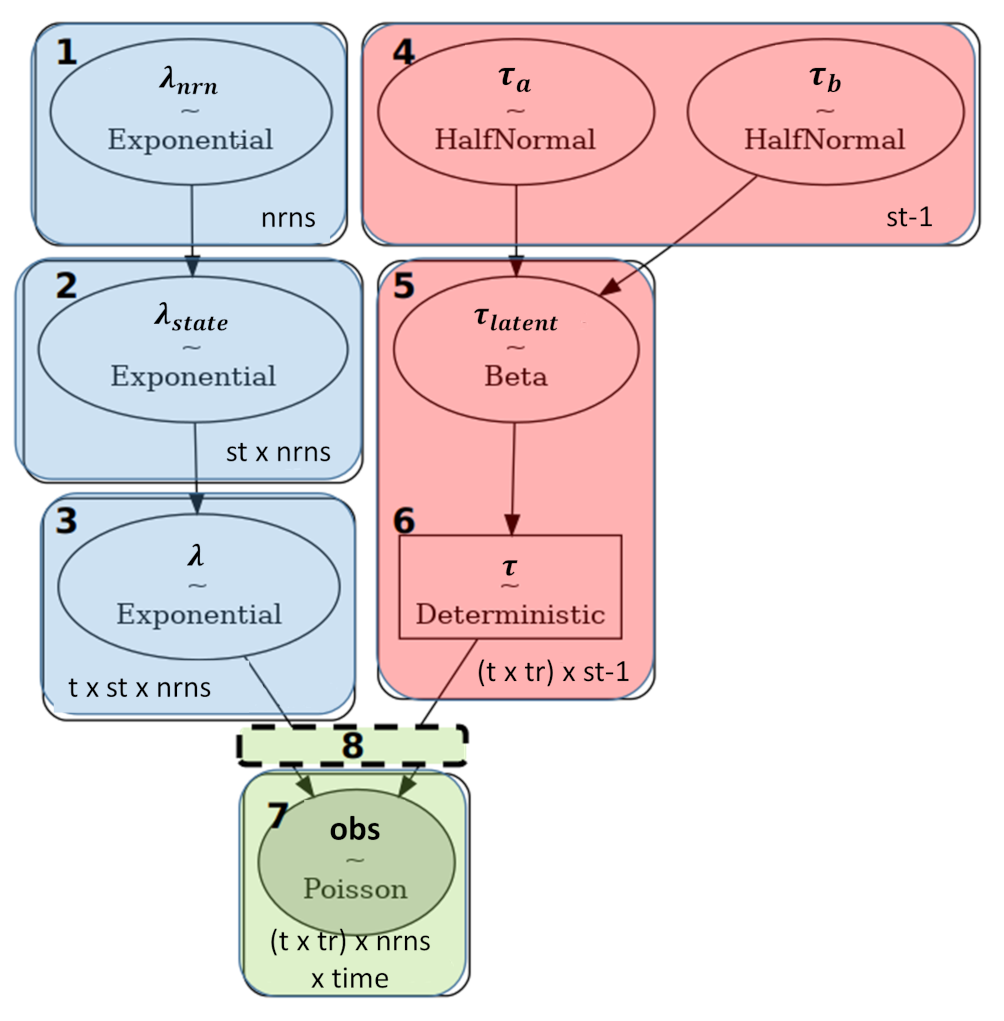
\includegraphics[width=\linewidth]{mahmood_22_figures/fig1-0.png}
\caption{\textbf{Dependencies between the random variables for constructing the changepoint model.} Different colors denote different parts of the model: Blue = Emission Variables, Red =Changepoint Position Variables, Green = Likelihood. Numbers on top left of each module (rectangle) correspond to the variable (equation) each module represents. Numbers on bottom right of each module correspond to the shape of the variables (and match with the shapes defined in the equations above). nrns = neurons, st = states, t = tastes, tr = trials, time = time bins}
\label{fig:wrapfig}
\end{figure}

\noindent\underline{Model fitting for GC.} GC ensemble taste responses have been repeatedly shown to involve sudden, coherent firing rate transitions. Because these transitions typically involve firing rate changes in approx. 50\% of the neurons in simultaneously recorded ensembles (\cite{jones2007a}), and because they are sudden and stark (see below), they can be observed in single trials using any of a number of methods (see \cite{mukherjee2019a}) and can be robustly inferred from ensembles as small as six neurons (\cite{jones2007a}). Here, a multi-changepoint model written in the probabilistic programming language pymc3 (\cite{salvatier2016a}) was used to determine the presence and latency of changes in ensemble responses.

\noindent It is important to note the uncertainty inherent in measuring the latency (and hence duration) of these transitions between hidden states using point process data (spike trains). This uncertainty is a function of the magnitude of firing rate changes, the noisiness of the spike trains themselves, and the number of simultaneously recorded neurons. Taking these constraints into account, previous work has shown (Sadacca et al., 2016) that the durations of transitions in recorded data are statistically indistinguishable from those observed using simulated data for which the underlying transition was by design instantaneous–i.e., for which the firing rates of simulated spike trains changed instantaneously at state transitions (note that the latency of these transitions were taken from analysis of experimental data, and therefore the simulations generated spike trains with PSTHs identical to those in the real data). Such analyses allow us to confidently conclude that the transitions detected in actual data (though they might appear longer due to noisy inference) likely correspond to instantaneous changes in the underlying firing rates of the neurons.

\noindent A detailed explanation of the change-point model structure and code used to identify ensemble transition times can be found online \href{https://github.com/abuzarmahmood/ pytau/blob/development/pytau/examples/Bayesian_Changepoint_Model.ipynb}{(GitHub)}. Briefly, taste-evoked spike trains (the 2000ms after stimulus delivery) were binned into 50ms bins. Poisson likelihood was used to model the binned spike counts. The model is broken down, in a manner similar to a Hidden Markov Model, into two sets of latent variables: 1) the emission variables (i.e. firing rates), and 2) the changepoint position variables (i.e. when changepoints occur). 

\noindent A single-neuron’s response to different tastes will be more similar than the responses of different neurons (even to the same taste). Equations 1-3 below hierarchically model firing rates (emissions) to exploit this similarity, such that the mean activity of each neuron is modelled independently \(\lambda_\text{nrn}\), Eq. 1), emissions for each state and neuron \(\lambda_\text{state}\) are dependent on \(\lambda_\text{nrn}\) (Eq. 2), and emissions for each taste, state, and neuron \(\lambda\) are dependent on \(\lambda_\text{state}\) (Eq. 3). This results in values of \(\lambda\) being drawn from a distribution of \(\lambda_\text{state}\) values, which in turn are drawn from distributions of \(\lambda_\text{nrn}\) values. This organization better constrains the space of emission values during different states for each neuron (i.e. the model knows the emission for State 1 for Neuron 1 will be similar to State 2 for the same neuron), allowing the model to fit more robustly. Equations 4-6 model the changepoint positions, assuming that the distribution of hyperparameters \(\tau\text{_a}\),\(\tau\text{_b}\) for a changepoint are shared across all trials for each given changepoint (e.g. hyperparameters for first transition is shared for the first transition across all trials, likewise the second transition, etc), but different for different changepoints. Finally, the latent emissions and changepoints are combined to generate timeseries of firing rates with sequential states (Eq. 8 is a deterministic function, refer to URL above for exact implementation), which is used to evaluate the likelihood of the data given the latent variables (Eq. 7). The dependencies between the equations are visualized in Fig. 1 below.
 
\noindent A modularized pipeline was used to fit and analyze the models across datasets (\href{https://github.com/abuzarmahmood/pytau/tree/development/pytau}{PyTau-GitHub}).

\noindent\underline{Model fitting for BLA. The same changepoint analyses} described above were also brought to bear on BLA ensembles, to test whether BLA population dynamics can be validly described, like those observed in GC, as transitioning suddenly and coherently. For these analyses, we used a separate cohort of 2 rats (9 recording sessions in total) in which we performed bilateral BLA recordings to obtain larger neural populations (results were qualitatively similar for those obtained from BLA-GC dual-region recordings). 

\noindent We compared goodness-of-fit for changepoint models fit to the recorded (actual) data with that for models fit to two surrogate datasets in which the single-trial coordination of the neural population was perturbed. To generate these surrogate datasets, we started with the actual observed spike train data, and either 1) randomly shuffled whole trials for single neurons (e.g., such that Trial 1 for one neuron was paired with Trial 4 for another neuron), or 2) shuffled individual spikes from one trial to the same time-bin in another trial for the same neuron. Both of these shuffling processes create datasets for which single-neuron PSTHs remain identical to the original, while disrupting any coherent changes in population activity present on single trials (see Fig. 4A).  

\noindent Model fitting was performed using Automatic Differentiation Variational Inference (ADVI, \cite{kucukelbir2016a}) capabilities present in pymc3. The ADVI algorithm optimizes the Evidence Lower BOund (ELBO) of the model. The ELBO is a lower limit on the marginal likelihood of the model (Blei et al., 2017); it automatically penalizes more complex models (which necessarily provide better apparent fits because they have more free parameters), allowing for model comparisons similar to the various Information Criteria. The ELBO is an integral part of the model fitting procedure, which makes it convenient and efficient to use as a tool for performing model comparisons. Statistical significance of differences between ELBO values for the actual data and shuffle conditions were determined using the 2-Way Repeated Measures ANOVA (from Pingouin) with Model States and Shuffle Type as factors.

\noindent\underline{Determining number of states}. Since a timeseries can be fit with a model containing an arbitrary number of states, we performed model comparison to determine the most parsimonious number of states to describe BLA taste ensemble activity (0-2000 ms post-stimulus delivery). We fit models with 2-10 states to each BLA population and used the ELBO for model comparison.  For each dataset, we ranked the different models using their respective ELBOs. 

\noindent\underline{Comparing transition-aligned changes in recorded activity to those in “smooth” surrogate data.} To supplement the above comparisons (and thereby further test and/or strengthen our conclusions), we compared the magnitude of firing rate changes across inferred changepoints in the actual data to that in the two above-described surrogate datasets. Given that these magnitude changes should be maximal only when changepoints are correctly identified at the ensemble level—i.e., when all neurons in the ensemble change their rates simultaneously in the trial—we would expect that changes in both single-neuron and population activity would be greater across inferred changepoints for the actual data vs the shuffled datasets. After inferring changepoints for models with 4 states (this number of states was determined to provide the best fit to our data; see Fig. 4), we computed the average firing rate in 500 ms bins on either side of each changepoint, calculating the magnitude of change across the changepoint for both single neurons and of the whole neural population (analyzed as changes in an instantaneous-activity vector comprised of all simultanteously-recorded neurons in a session). To compare both the average magnitude and pervasiveness of differences between activity in the datasets (to enhance conservativeness by accounting for the few large outliers skewing average changes in magnitude), we calculated: 1) The number of neurons for which, on average, the actual data had larger magnitude of change across the transitions; 2) the number of neural populations for which the actual data had a larger magnitude of change across the transition; 3) the fold-change of magnitude in firing for single neurons (shuffled data/actual data); and 4) the fold change in magnitude of the population vector. The number of larger neural transitions was calculated by assessing which group (actual data, whole-trial shuffle, spike-trial shuffle) had the largest change in activity across the transition, for every transition; this produces ratios for which group he largest transition belonged to.

\noindent Testing for significance of the likelihood that transitions  are larger in the recorded data than in control simulations (points 1 and 2 above) was carried out using a One-Way ANOVA followed by Tukey’s post-hoc test. Hypothesis testing for differences in magnitude was performed using Wilcoxon signed-rank test with Bonferroni’s correction (points 3 and 4 above). 

\noindent\underline{Coordination of BLA and GC Transition Times}
To test our central hypothesis regarding the coupling of BLA and GC transitions in single trials, we assessed synchronization of transition times using simple correlative statistics.

\noindent\underline{Testing transition-time correlation as a coordination metric.} To test the utility of this approach, we first performed pilot analyses on GC ensembles (which are known to transition suddenly) with higher counts of simultaneously recorded neurons (n\(\ge\)10neurons/population). We divided these ensembles into two populations randomly, repeating the splits 10 times/ensemble to avoid any issues related to selection of unrepresentative groups. Transition times were inferred independently for each half-ensemble (using techniques described above), after which the values for transition times in the two halves were correlated (Spearman’s Rho). The significance of these correlations was tested as described for the BLA-GC inter-regional correlations below.
BLA-GC transition time synchronization. Coupling between BLA and GC transition times were assessed as described above. Transition times were inferred independently for simultaneously recorded GC and BLA ensembles. Statistical significance of each correlation was determined at the single transition level, and also by aggregating across all experimental recordings. 

\noindent At the single transition level, the correlation coefficient of each transition was compared to the distribution of coefficients calculated by trial-shuffling the data (1000 shuffles per each correlation) and deemed “strongly correlated” if it was more highly correlated than 90\% of the trial-shuffled datasets. To determine whether the correlations we see across all recordings and transitions are collectively (i.e., at the aggregate level) significant, we determined the fraction of strong correlations for all datasets, and compared this number to the fraction expected from random data. The fraction of significant correlations for random data was generated using trial-shuffled data similar to the single-transition correlation comparison; however, in this case, shuffled data were generated up to the number of transitions present in the original data (creating a dataset of the same size as the actual dataset, but with shuffled data). The fraction of significant correlations was counted for this shuffled dataset, and the process repeated x1000 times. This provided us with a distribution for “Fraction of Significant Correlations” expected from random data, and the fraction present in the actual data compared to this shuffle distribution. The p-values for transitions in the actual data were calculated using the percentile relative to this shuffle distribution. Values from actual data were deemed significantly different if they had p<0.05 for one-tailed comparisons with Bonferroni’s correction against the shuffled distribution. For completeness, this was followed-up with a Binomial test with alpha = 0.05 (with Bonferroni’s correction). The two tests gave identical results.

\noindent\underline{Investigating the relationship between changepoint uncertainty and transition correlation strength.} As alluded to above, uncertainty in estimating the timepoint of transitions limits the calculated correlation strength of transitions across populations (thus causing potential underestimation of BLA-GC transition coupling). This uncertainty is an inevitable result of inferring state changes from noisy firing rates. Because we use a Bayesian model, we are able to quantify the uncertainty in a transition latency estimate, in the form of the variance of the posterior distribution of the transition position \(\tau\). To assess the degree to which this uncertainty in changepoint position impacted the calculated BLA-GC transition correlation strength, we used the trial-averaged variance of transition posterior distributions, summed across regions, as a proxy (η) for the uncertainty contribution from each neural population (BLA/GC, see below).
 
\noindent Once calculated, η was then linearly regressed against its respective correlation coefficient to determine the strength of the relationship. Significance of this relationship was determined using 2-tailed Wald’s Test with T-distribution.

\smallskip
\noindent\textbf{Netowrk model with staet specific coherence}\par
\noindent\underline{Network Model Simulation}We instantiated a simple network simulation to test whether groups of neurons, that were by definition coupled, produce responses with the properties observed in our BLA/GC recordings. Conceptually, the model is a firing rate model, containing four units, each representing an ensemble of similarly responsive mixed excitatory and inhibitory cells, with the mean rate of each group being the relevant variable. Units are connected first as pairs, with each pair representing one unit from GC and one unit from BLA. Within these cross-regional pairs, the connectivity is set up like that of an oscillator with strong self-excitation within one unit, and cross-connections being excitation in one direction and feedback inhibition in the other. It happens that the pairs do not spontaneously oscillate, but oscillatory-like activity is produced by the uncorrelated background noise added to each unit. One of the pairs has stronger cross-connections and is closer to being an inherent oscillator than the other pair, resulting in greater coherence in the activities of one pair than the other. Finally, the connections from one pair to the other are inhibitory, such that one pair’s activity suppresses the others and vice versa. Noise causes occasional spontaneous transitions between states, with each state consisting of one cross-regional pair of active units.  For a graphical representation of the model structure, see Fig. 10A.

\noindent Specifically, each model unit, i,  has a firing rate, \(\text{r_i}\), which responds linearly to its total input, \(\text{I_i}\) and varies according to:
$$\tau (dr_i)/dt=-r_i+I_i-T_i, r_i\ge0$$
where \(\text{T_i}\) is a threshold, indicating the minimum input needed for activity, or (if negative) its magnitude indicating the level of spontaneous activity in the absence of input. Importantly, since rates cannot be negative, we enforce r_i\(\ge\)0 whenever the above dynamical equation would indicate otherwise. The input current to each unit is given by the weighted sum of connected units plus an independent white noise term:
$$I_i (t)=∑_i▒〖W_ji r_j (t) 〗+\(\sigma\)^I η(t)$$
where \(\sigma\text{^I}\) is the standard deviation of the noise and η(t) is an uncorrelated white noise term with zero mean and unit standard deviation, 〈η(t)〉=0 and 〈η(t)η(t')〉=δ(t-t').
Values of the parameters are given in Table 1 below. Simulations were carried out in MATLAB (R2018a) using the Euler-Mayamara method for integration. Code is freely available online at https://github.com/primon23/Two_State_Oscillators .

\noindent\underline{Phase Coherence for Network Model}
The simulation described above was used to generate 20 trials of neural activity. The activity of both units in each “region” was summed to produce a single time-series which was treated as an analog for LFP. This LFP was then bandpass filtered (10-40 Hz) and subjected to a Hilbert transform, and instantaneous phase was estimated using the analytical signal from the transform. Since latencies of state transitions in the simulated activity are random (unlike experimental data where they are roughly bounded in latency and occur in a sequential order, a fact likely related to the model’s omission of biological processes with longer time constants, like synaptic depression/facilitation or firing rate adaptation), we calculated phase coherence for the simulated data in each state using windows of activity centered around the transition from the moreless coherent state. Data across trials were aligned to state transitions from the moreless coherent states and snippets with radius = 350ms (minimum duration of states across all trials) of the LFP phase were taken around the transition time. Inter-trial phase coherence calculation was performed on these aligned snippets as described above.

\smallskip
\noindent\textbf{Data Availability}\par
\noindent We have structured our electrophysiology datasets in a hierarchical data format (HDF5) and are hosting the files on a university-wide network share managed by Library and Technology Services (LTS) at Brandeis University. These HDF5 files contain our electrophysiology recordings, sorted spikes, single-neuron and population-level analyses (and associated plots and results). These files are prohibitively large to be hosted on a general-purpose fileshare platform - we request anyone interested in our datasets to contact the corresponding author, Donald Katz (dbkatz@brandeis.edu) who can put them in touch with LTS in order to create a guest account at Brandeis through which they can securely access our datasets (hosted on the katz-lab share at files.brandeis.edu). Code to perform the network model simulations can be found at https://github.com/primon23/Two_State_Oscillators.

\section{Results}
In order to appropriately contextualize our novel central hypothesis and analysis, we build the following accounting of the Results in a step-by-step manner. We start by replicating/confirming basic results from our prior work (Figs. 2 & 3) and move on to testing basic questions concerning whether BLA responses show within-trial firing-rate transitions that could conceivably be coupled with those of GC (Fig. 4 & 5). From there, we move on to using field-standard techniques to test whether GC and BLA responses show simple trial-to-trial coherence (Fig. 6), and whether coherence changes from one response epoch to the next (Figs. 7 & 8). Once epoch-specificity of response coherence is established, we move on testing whether BLA-GC coupling during taste processing is specifically instantiated in the synchrony of transitions into and out of the GC palatability-related epoch, and whether the entirety of these phenomena is truly consistent with the function of tightly coupled networks (Figs. 9 & 10).

\subsection{Simultaneous single-neuron ensemble recordings from BLA and GC}

\begin{figure}
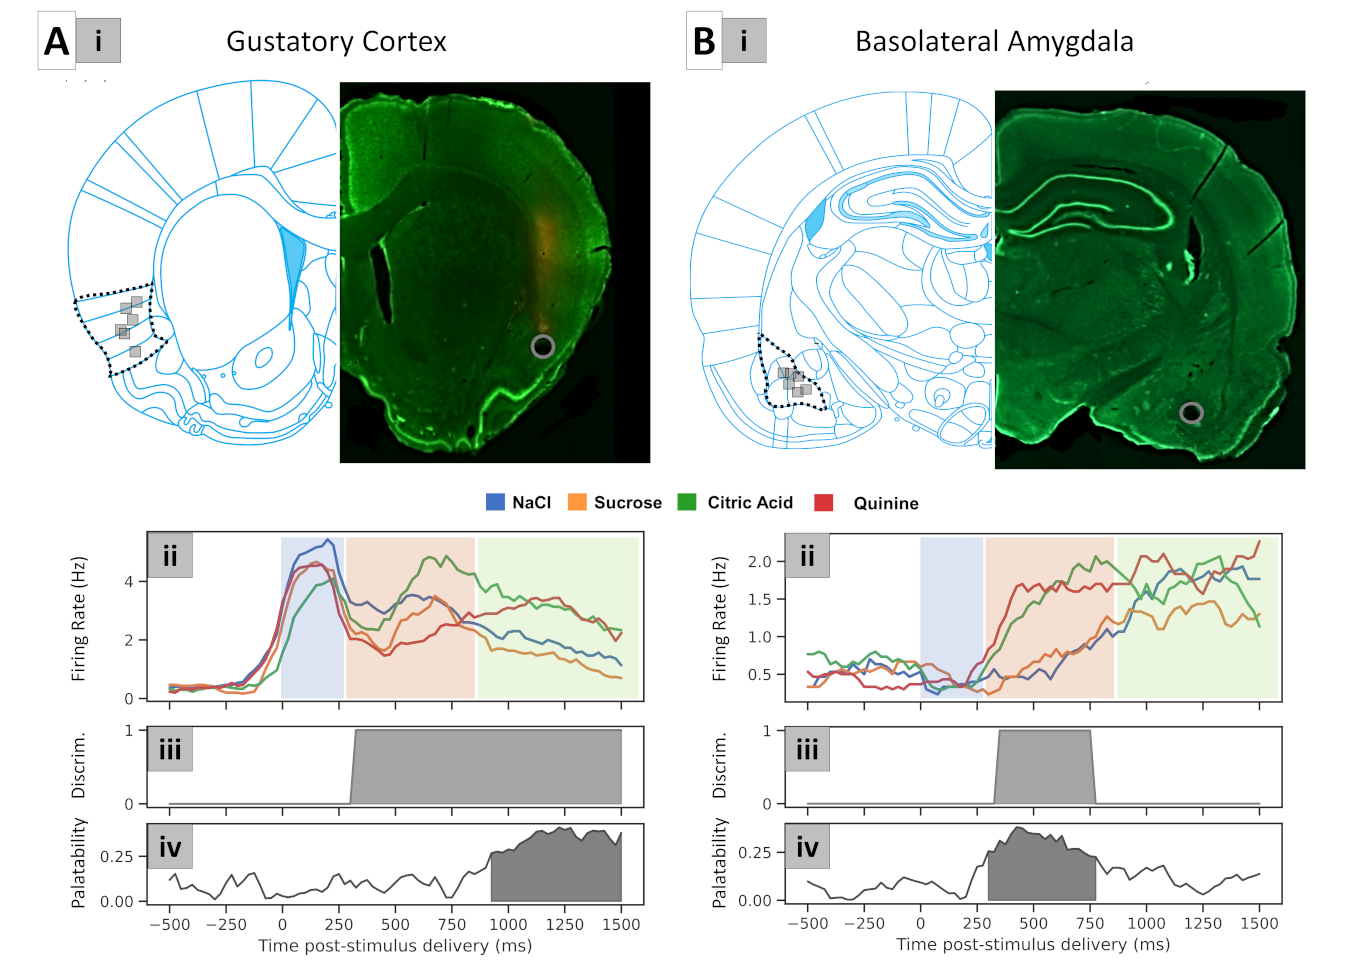
\includegraphics[width=\linewidth]{mahmood_22_figures/fig2-0.png}
\caption{\textbf{Histology and example PSTHs from recorded regions.} Column \textbf{A} is GC; column \textbf{B} is BLA. \textbf{(i)} Schematics and sample histology (x2 magnification) showing electrode bundle placements. Brain slices were registered to brain atlas schematics at 1.4 mm anterior to bregma for GC and 3.00 mm posterior to bregma for BLA. Dashed lines outline GC and BLA, with gray squares showing the final locations of each electrode bundle. Gray circles in the photomicrographs outline electrolytic lesions (schematics were modified from Paxinos, 2007—permission will be requested from Elsevier upon the publication).  \textbf{(ii)}: PSTHs for representative GC and BLA single-neuron responses to each taste. Previously described response epochs (e.g., Katz et al., 2001) are denoted with different colored shading behind the PSTHs. \textbf{(iii)}  Boolean timeseries reflecting whether neural activity significantly differentiates tastants (0 = no, 1 = yes) at a particular time point, with shading emphasizing periods of significant differences among responses. \textbf{(iv)} Correlation of neural activity with taste palatability (see Methods) through time; shaded regions denote periods of significant correlation.}
\label{fig:wrapfig}
\end{figure}

We isolated multiple single neurons simultaneously from both GC and BLA in 6 rats. Electrode bundle tip placements are shown in the top panels of Fig. 2: a coronal schematic of the regions (GC Fig. 2A.i, BLA Fig. 2B.i), with the locations of all bundle tips marked, is displayed in the left half of each panel; the right half of each panel is a photomicrograph showing an example placement. 

The rest of Fig. 2 presents representative recordings from each region. Fig. 2A.ii and B.ii show overlain peri-stimulus time histograms (PSTHs) of example GC and BLA neuron responses to each taste. The colors behind the PSTHs show the average periods of GC coding epochs described previously (\cite{katz2001a,fontanini2009a,sadacca2012a}). Note that both GC and BLA responses re-arrange themselves (i.e., the ordering of which tastes induce the larger/smaller response magnitudes changes, y-axis) around the times of epochal boundaries. The nature of the “coding” performed by each neuron changes with these epochal re-arrangements, as well (\cite{katz2001a,sadacca2012a,moran2014a,li2016a}); in GC, the early epoch has little taste specificity, but the middle epoch responses “code” at least a subset of tastes distinctly, and in the late epoch responses become generally organized by palatability (note, for instance, in Fig. 2A.ii that the late response is ordered from most aversive to most palatable—the strongest response is to quinine, followed in order by citric acid, NaCl, and sucrose). In BLA, meanwhile, palatability-related responses appear in the middle epoch, and (unlike the GC responses) primarily reflect strong responses to tastes of only one (in this case, negative) valence; both of these aspects of BLA taste responses replicate previous investigations (\cite{fontanini2009a}).

These findings are statistically confirmed by analyses summarized in the panels below the PSTHs. The middle row (“Discrim” in the y-axis, Fig. 2A.iii and B.iii), which plots the significance (p<0.05) of a moving window of ANOVAs for Tastes, reveals that the responses displayed in Fig. 2A-B.ii become distinctly taste-specific starting at approximately 250 msec after taste delivery (i.e., at the start of the 2nd epoch; the BLA neuron stops doing so at the end of this epoch); the bottom panels (“Palatability”, Fig. 2A.iv and B.iv) which plot Pearson’s R between the known palatability of each taste and the neuron’s response to each taste—i.e., the correlation (shaded region, p<0.05) between the two variables—show that the palatability-relatedness of the GC responses becomes significant a little before 1000 msec after taste delivery (i.e., at the onset of the 3rd [late] epoch), and that the palatability-relatedness of the BLA responses is significant for the one-epoch  entirety (middle epoch) of the taste-specific response. Again, these results confirm findings published in multiple previous papers (\cite{katz2001a,grossman2008a,fontanini2009a,sadacca2012a}), and motivate our basic hypothesis that the systems-level mechanisms of taste coding will intrinsically involve epoch-specific processes.

A good deal of previous research has demonstrated that taste-response epochs translate into this sequence of states (each lasting hundreds of msec) in single-trial evoked GC ensemble activity (\cite{jones2007a,sadacca2016a,mukherjee2019a}), separated by sudden (50-200 msec) coherent firing-rate transitions (spontaneous GC activity also contains such transitions; see \cite{camera2019a,mazzucato2015a}). We note here that we use the term “epoch” to describe periods of distinct activity seen in single neuron PSTHs (Fig. 2), whereas “state” is a term borrowed from modelling literature and is used here to describe simultaneous changes in the recorded neural population activity while accounting for temporal variation at the single trial level. However, since state transitions correspond to epoch transitions across trials (on average, see Fig. 9C and D for a comparison of average state-transition times in our data and previously shown epochal-transition times), it is sometimes difficult to cleanly delineate single-trial from trial-averaged analyses; in these cases, we use the term that seems most appropriate.

These state transitions represent an integral part of neural activity, in that they both predict the onset of (\cite{sadacca2016a}) and drive (\cite{mukherjee2019a}) consumption-related behavior—that is, rather than being trivial reflections of mouth movements, the dynamics represent the processing of tastes that leads to discriminative mouth movements (see also (\cite{jones2007a,katz2001a}). The seeming “ramping onset” of the above-described late epoch containing palatability-related firing (see Fig. 2) proves to be an artifact of averaging across the large trial-to-trial variability (on the order of hundreds of milliseconds) in the latency of this sudden transition (\cite{jones2007a,sadacca2016a}). Furthermore, because this phenomenon is not sparse—approximately 50\% of the neurons in an ensemble will change their firing rates at any particular transition—it can be reliably observed in sub-ensembles as small as 6 simultaneously-recorded neurons (\cite{jones2007a}). 

\begin{figure}
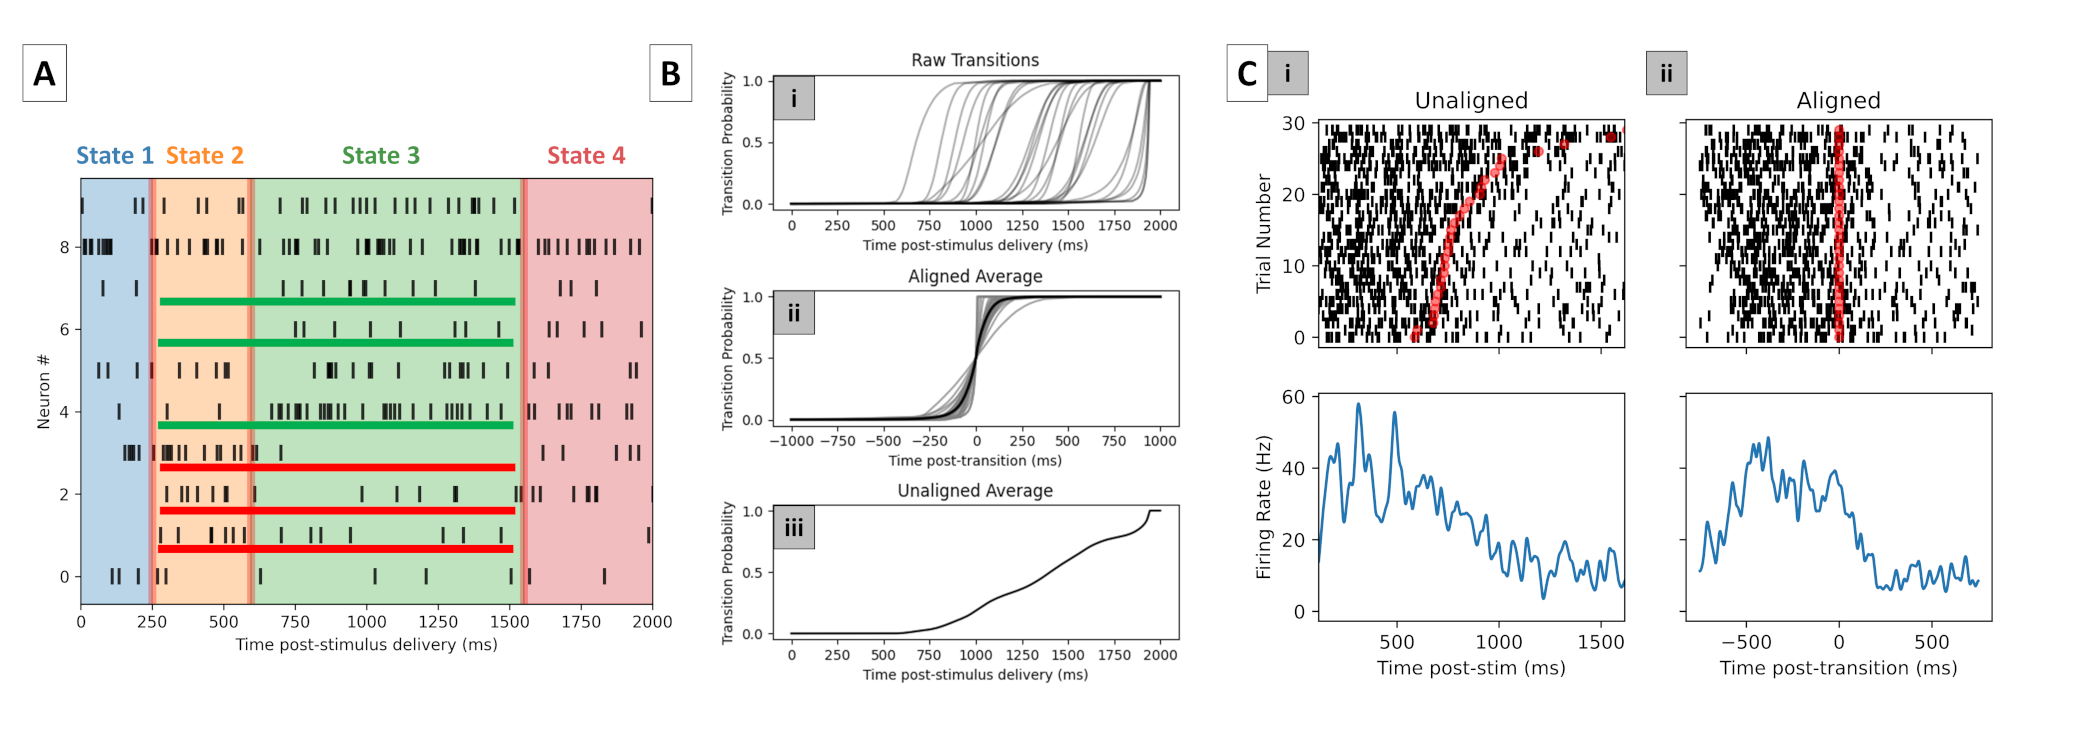
\includegraphics[width=\linewidth]{mahmood_22_figures/fig3-0.png}
\caption{\textbf{GC evoked population activity contains sudden state transitions.} \textbf{(A)} A single trial of GC taste-evoked activity in 10 simultaneously recorded single neurons. Inferred states (here identified using an ensemble change-point algorithm) are indicated in overlain shading. For the transition leading into the period of palatability-related activity (i.e., from State 23), spike trains that increased in firing rate are underlined in green, and spike trains that decreased in firing rate are underlined in red. \textbf{(B) (i)}  Identified time-courses for the State 23 transition in 30 trials for a single ensemble. \textbf{(ii)} aligning the middle (i.e., 0.5 probability) of the transitions shows that they typically occur suddenly. \textbf{(iii)} when averaged across data synchronized to stimulus onset, however, the transition appears smooth and slow (similar to neural activity in trial-averaged PSTHs). \textbf{(C) (i)} The raster plot (above) and PSTH (below) for a single, representative GC neuron that shows a sudden decrease in its firing rate occurring at variable latencies across trial. The time of the transition, inferred by the change-point algorithm on activity of the entire simultaneously recorded ensemble, is shown with a red hash mark. \textbf{(ii)} By aligning activity to calculated transition times (producing a “peri-transition time histogram”), the sharp decrease in neural activity across the transition can be better appreciated.}
\label{fig:wrapfig}
\end{figure}

Once again, the current data replicate these findings (Fig. 3), showing that even a small ensemble of simultaneously-recorded GC neurons (here, 10—again, almost 2x the number of neurons needed to resolve this phenomenon; (\cite{jones2007a})) can be observed to undergo sudden, coherent firing-rate changes in the process of responding to tastes (Fig. 3A). The states and state transitions identified by our change-point algorithm are overlain on the ensemble raster plot, and the 6 (of 10; 60\%) neurons that significantly increased or decreased their firing rates at the time of the transition into the 3rd (putative palatability-related) state are indicated with green or red lines, respectively (note the sudden increase in the rate of spiking in neurons 4, 6, and 7, and the simultaneous decrease in firing rate in neurons 1, 2, and 3) under their spike trains. The algorithm was able to progress to near-perfect confidence in the transition across an extremely short time interval in almost every trial (Fig. 3B.i), which is to say that these changes in neural activity are, on average, very sudden on a single-trial basis (Fig. 3B.ii); because the latency of the transition could vary wildly from trial-to-trial (Fig. 3B.i), however, the onset of the post-transition state appears to be a slow-ramping onset of the late epoch when averaged across trials synchronized to stimulus delivery (Fig. 3B.iii). 

Once calculated from the ensemble data, the time of transitions could then be used to directly illustrate the sharpness of the firing-rate changes in even single-neuron data. Fig. 3C shows a representative GC neuron: note that the firing-rate change that seems like a slow ramp in data synchronized to stimulus delivery (Fig. 3C.i: “Unaligned” rasters above and associated peri-stimulus time histogram below) is in fact precipitous when the trial-to-trial variability of that change’s latency is accounted for (Fig. 3C.ii: “Aligned” rasters and associated peri-transition time histogram). Keep in mind that this change is not caused by the stimulus being removed from the tongue: it occurs at least a full second before swallowing, and both precedes and reliably predicts (\cite{sadacca2016a}), as well as participates in driving (\cite{mukherjee2019a}) discriminative oral behaviors.

\subsection{BLA activity contains trial-specific, sudden ensemble firing-rate transitions}
Having re-confirmed that GC epochal dynamics reflect sequences of single-trial states, and en route to assessing the coordination between BLA and GC neural responses and testing our hypothesis that BLA state transitions are coupled to those in GC, it is necessary that we determine whether the sort of nonlinearities in firing rate which have been extensively described in GC (Fig. 3; see also \cite{jones2007a,sadacca2016a}) also truly characterize BLA taste responses. That is, we must first test whether evoked BLA activity, which involves epochal dynamics that are similarly timed to those in GC (see Fig. 2 for single-neuron examples of the similarity between BLA and GC dynamics; see also \cite{fontanini2009a}), are well described as sudden ensemble state transitions in single trials. Only if the population dynamics of BLA taste-evoked responses also consist of sudden transitions between a small number of ensemble states (a hypothesis that has not yet been tested) is our most novel hypothesis tenable.

To this end, we evaluated the spiking activity of BLA ensembles using the same changepoint model designed to detect coherent ensemble transitions in GC data. To ensure robust sampling of BLA population activity, this set of analyses was performed on data from a separate group of animals with bilateral BLA electrode implants (2 animals, 9 recording sessions; however, all results reported in this analysis were qualitatively similar to those obtained using unilateral BLA populations taken from BLA-GC dual region recordings—see below). First, we fit a battery of models containing 2-10 states to the evoked responses from the BLA ensembles, and compared the goodness-of-fit of the probabilistic models (quantified using the ELBO; see Methods) to that of identical analyses performed on control datasets made by shuffling either whole trials or single spikes between trials for the same neuron (both manipulations preserve the across-trial dynamics and have equivalent PSTHs to the actual data; Fig. 4A). Performing this set of analyses allowed us to test whether the real data were better fit by the sudden transition model than one would expect by chance. We predicted that the unmanipulated data would achieve a higher goodness-of-fit to the sudden state change model.

\begin{figure}
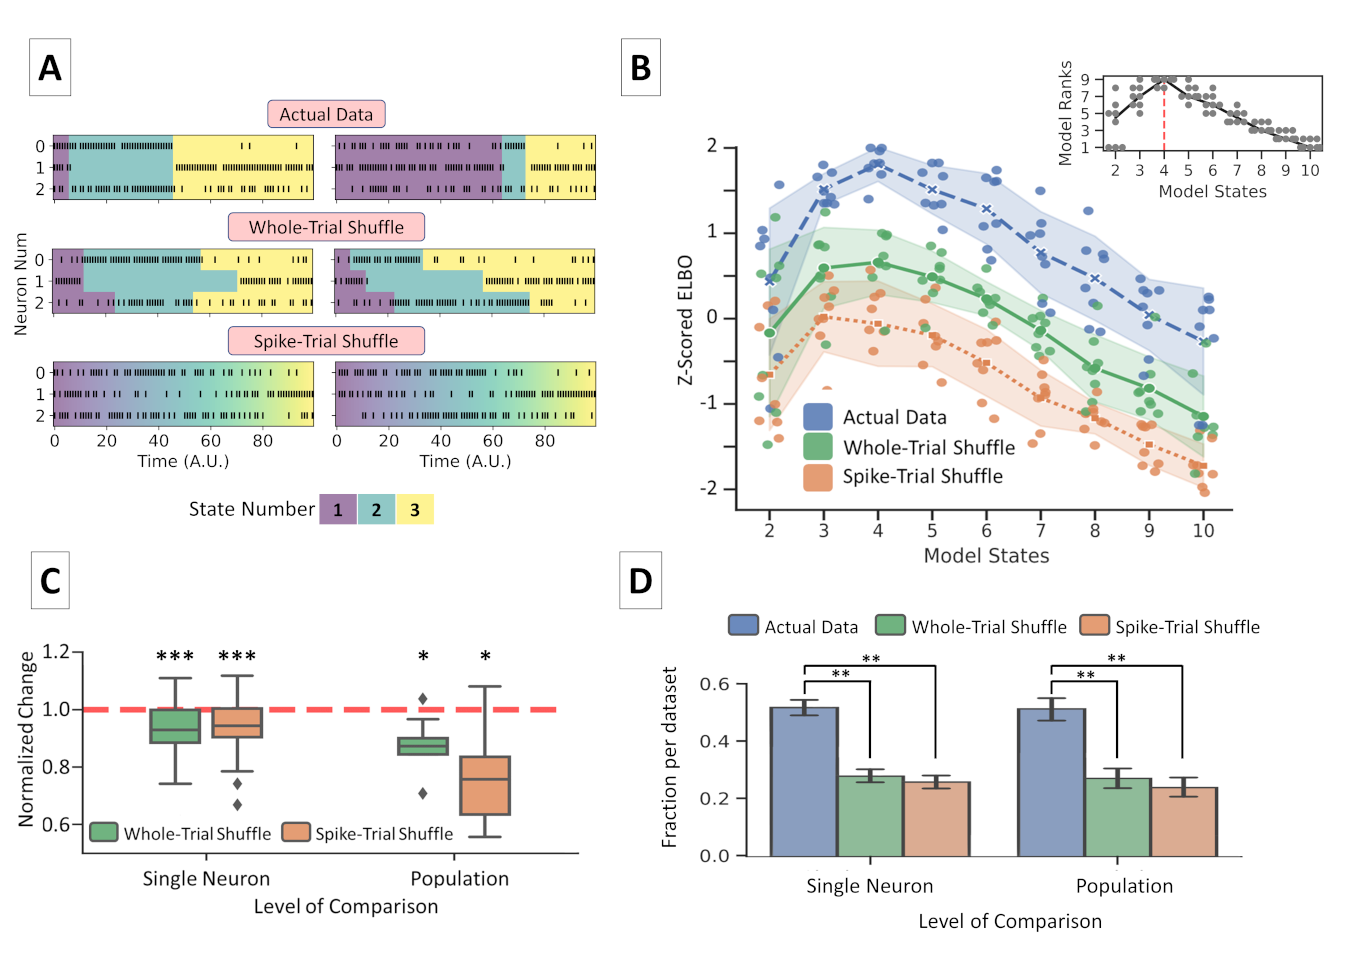
\includegraphics[width=\linewidth]{mahmood_22_figures/fig4-0.png}
\caption{\textbf{BLA population responses can validly be characterized as progressing through a sequence of state transitions.} \textbf{(A)} Visualization of how the actual data were transformed by the different shuffling procedures. Raster plots are overlayed with colors identifying states for the neural population; two trials (one in each column) are shown. Actual Data: State-transitions are hypothesized to occur coherently across all neurons for the same trial. Whole-Trial Shuffle: State-transitions are mismatched between neurons on the same trial. Spike-Trial Shuffle: Sharp, trial-variable state-transitions have been destroyed by changing in which trial each particular spike occurred, largely leaving smooth changes in the neural activity which are consistent across trials. A.U. : Arbitrary Units  \textbf{(B)} ELBO values for 2-10 state models fit to the actual data and surrogate datasets. Note that the ELBO (unlike model likelihoods) penalizes more complicated models, allowing us to visualize peak fit rather than seeking an actual elbow in monotonically increasing functions. Inset) Ranks for models with 2-10 states. Models with 4 states consistently show the highest ranks across the dataset. Solid black line shows median rank per state. \textbf{(C)} Comparison of average, normalized changes in single-neuron and population vector firing rates in the vicinity (from 500ms before to 500 msec after) of transitions. Firing-rate changes across transitions are consistently diminished by shuffling, a decrement that is particularly noticeable at the population level. Edges of boxes show 1st and 3rd quartiles, and the horizontal line through the boxes shows the median. The dashed red line denotes the (normalized) firing-rate changes in the actual data. * = p<0.05, *** = p<0.001, for mean value is different from 1.0 \textbf{(D)} Comparison between actual data and shuffled surrogate datasets for which dataset contained the higher number of "larger“ transitions. Unperturbed BLA datasets consistently had more transitions with largest changes in firing rate (Mean ± SEM, **: p<0.01).}
\label{fig:wrapfig}
\end{figure}

This analysis revealed that models with 4 states had the highest ELBO—that 4-state models best describe BLA population activity for the 2000ms of post-stimulus activity we have used in this study (Fig. 4B, see Table 2 for statistics used to test these effects). Note that only 3 of these states typically appeared in the first 1500 msec—that is, in the period leading up to and including the GC “palatability-related” state—and that while we are interested in the transition out of that “palatability-related” state, we are not yet prepared to interpret the state following (which is post-decision). This number of states accords well with results from HMM modeling of GC activity (\cite{jones2007a,sadacca2016a}), supporting our suggestion that GC and BLA taste-response dynamics are similar in kind (and demonstrating that these results hold across very different analysis techniques). Furthermore, this fit was significantly higher (as was the relative advantage of the 4-state model) than that achieved by even the trial-shuffled surrogate dataset (F(2,20)=26.9, p=2.13x10-6, 2-way repeated measures ANOVA for Shuffle Type and Number of States, n=9 recordings across 2 animals), which left each trial’s spike trains intact (Fig. 2), eliminating only the between-neuron coherence of single-trial dynamics. 

We further evaluated the BLA ensemble data by comparing the magnitude of firing rate changes across state transitions identified by this optimal 4-state changepoint model (see Sadacca et al., 2016 for similar analysis of GC responses), compared to those observed in surrogate datasets. We predicted that both the average magnitude of transition-aligned changes in firing rates and the quantity of transitions showing larger changes in firing would be higher for the “actual” data than for the surrogate datasets in which we disrupted the coherence of single-trial changes in population activity. Our results confirmed these predictions: compared to the surrogate datasets, neurons and ensembles in the actual, unmanipulated BLA data showed consistently larger changes in firing rate across transitions (Fig. 4C; see Table 2 for an accounting of the extensive statistical analyses used in these tests); furthermore, the percentage of BLA single neurons and ensembles for which changes in firing rate across transitions were largest in the actual data was more than twice that for either shuffled dataset (Fig. 4D; again, see Table 2). 

These findings suggest that BLA ensemble taste responses are well described as consisting of sudden, coherent firing-rate transitions in single trials. Fig. 5A shows a representative ensemble taste response from 8 simultaneously recorded BLA neurons that clearly involves rapid state transitions, one of which occurs at around the average time of GC transitions into palatability coding (see Fig. 2); at this transition, 5 out of 8 neurons underwent either an increase or decrease of firing rate simultaneously (for another, neuron #3, the increase was almost but not quite significant). As in GC (Fig. 3; see also \cite{jones2007a,sadacca2016a}), these transitions were variable in latency across trials (Fig. 5B.i), such that while the average transition time was brief (Fig. 5B.ii), averaging across trials synchronized to stimulus delivery made that transition time appear artifactually slow (Fig. 5B.iii).

\begin{figure}
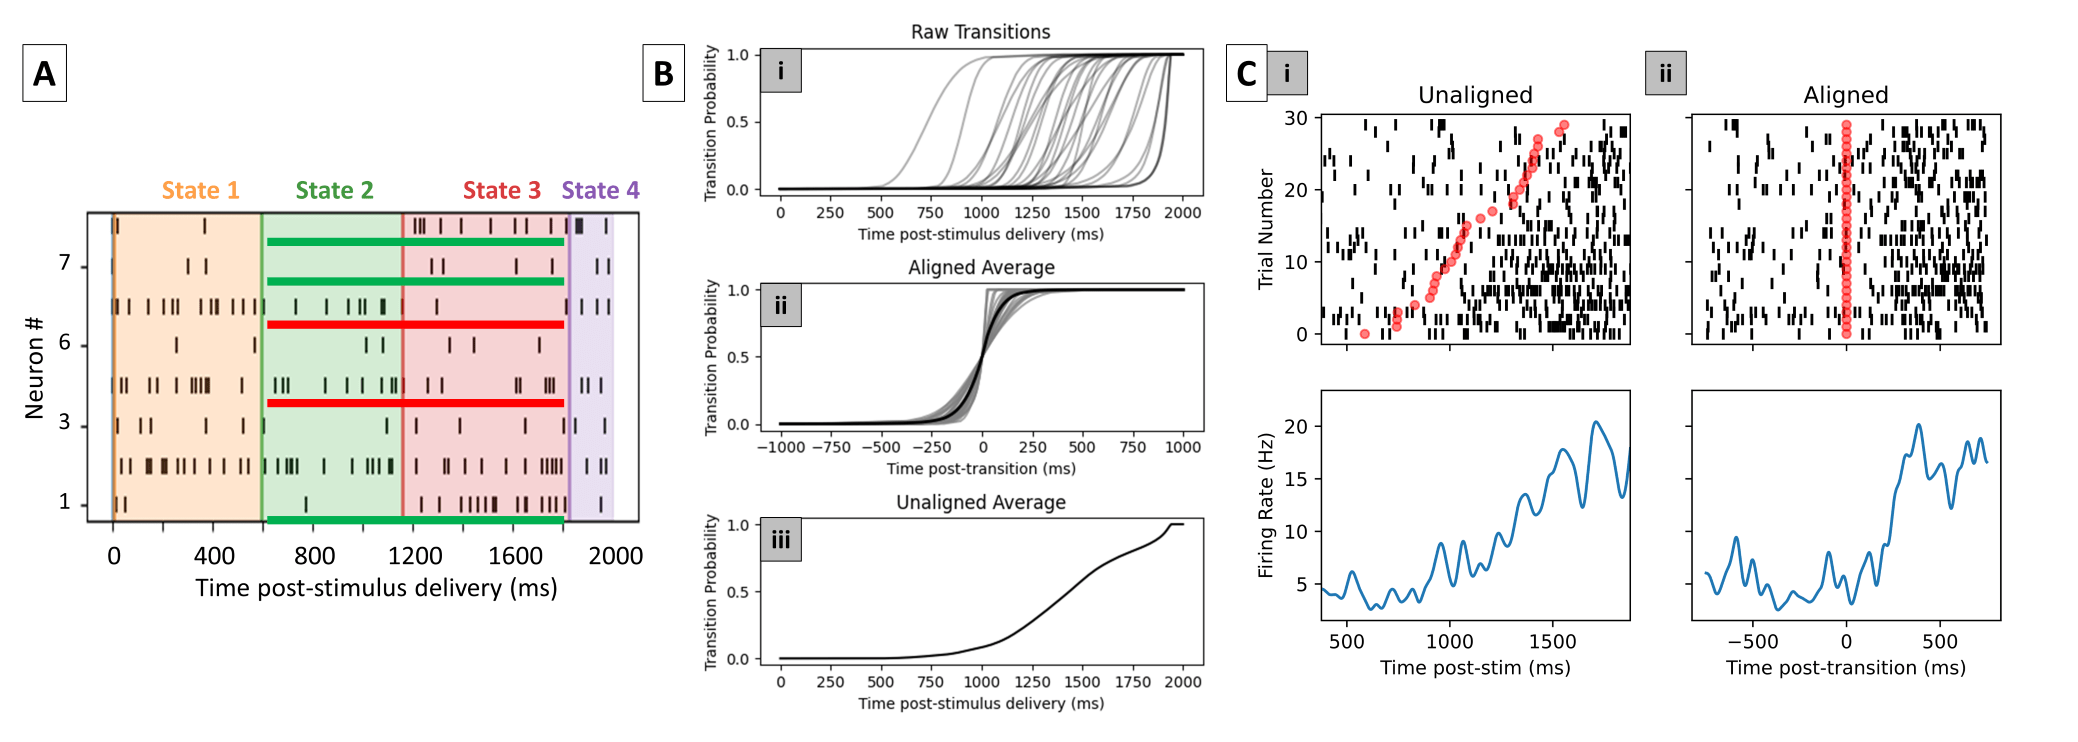
\includegraphics[width=\linewidth]{mahmood_22_figures/fig5_corrected_rescaled.png}
\caption{\textbf{BLA evoked population activity contains sudden state transitions. (A)} A single trial of BLA taste-evoked activity in 8 simultaneously recorded single neurons. Inferred states (here identified using an ensemble change-point algorithm) are indicated in overlain shading. For the transition leading into the period of palatability-related activity (i.e., from State 23), spike trains that increased in firing rate are underlined in green, and spike trains that decreased in firing rate are underlined in red. \textbf{(B) (i)} Identified time-courses for the State 23 transition in 30 trials for a single ensemble. \textbf{(ii)} aligning the middle (i.e. 0.5 probability) of the transitions shows that they typically occur suddenly. \textbf{(iii)} when averaged across data synchronized to stimulus onset, however, the transition appears smooth and slow (similar to neural activity in trial-averaged PSTHs). \textbf{(C) (i)} The raster plot (above) and PSTH (below) for a single, representative BLA neuron that shows a sudden increase in its firing rate occurring at variable latencies across trial. The time of the transition, inferred by the change-point algorithm on activity of the entire simultaneously recorded ensemble, is shown with a red hash mark. \textbf{(ii)} By aligning activity to calculated transition times (producing a “peri-transition time histogram”), the sharp increase in neural activity across the transition can be better appreciated.}
\label{fig:wrapfig}
\end{figure}

Finally, we again fed back the results of this ensemble analysis to directly illustrate the sharpness of single-neuron firing changes across transitions. Fig. 5C shows, for one representative BLA neuron, that firing-rate changes that seem like slow ramps in data synchronized to stimulus delivery (Fig 5C.i; “Unaligned” rasters and associated peri-stimulus time histogram) are in fact precipitous when the trial-to-trial variability of that change’s latency is accounted for (Fig 5C.ii; “Aligned” rasters and associated peri-transition time histogram). While we have no current explanation for the apparent slight delay in this particular BLA neuron’s firing-rate change (we suspect that the answer lies in compromises made by the algorithm in settling on a “best guess” of transition time), it is clear that BLA ensembles, like GC ensembles, respond to tastes with sequences of states separated by sudden state transitions.

\subsection{BLA and GC responses show strong trial-to-trial coherence}
The above data motivate our hypothesis that taste processing involves BLA-GC coupling of the brief transitions into the state that, in GC, predicts and controls consumption behavior. But given that the vast majority of published studies assessing multi-region coordination have done so not in terms of momentary coupling—they have instead focused on multi-second responses, with quantification performed via evaluation of the magnitude of correlation between spike counts in simultaneously-recorded pairs of neurons (\cite{averbeck2006a,averbeck2006b}), or alternatively via evaluation of similarity in local field potentials (LFP) simultaneously recorded from the regions under investigation (\cite{place2016a})—we first assessed whether GC taste processing is coherent with that of BLA according to these standard metrics. To maximize our ability to compare our results to those of these earlier studies, we began our investigation of BLA-GC taste-response coupling by looking at these broader measures, and then moved on (in the following sections) to testing the epochal specificity of this coherence, a result that would more directly motivate our ultimate test of the hypothesized synchronous transitions BLA-GC transitions into the behaviorally-relevant state.

We first considered the trial-wise strength of coordination between BLA and GC, by investigating trial-to-trial spike-count correlations (using the 0-2000 ms post-stimulus time-period, which is the period of the most prominent taste-evoked response) for every simultaneously-recorded BLA-GC pair of neurons, thereby testing the broad hypothesis that BLA and GC responses rise and fall in a correlated (or anti-correlated) manner from trial-to-trial. The two example GC-BLA neuron pairs shown in Fig. 6A in fact demonstrate strong coherence on this time scale: the trial-to-trial firing rates of the pair on the left are (significantly) anti-correlated, a fact that can be particularly well appreciated in the scatterplot of BLA and GC firing rates (each dot reflects one trial) below the trial-to-trial chart of responses; the pair to the right is similarly (albeit in this case positively) correlated. 

\begin{figure}
\centering
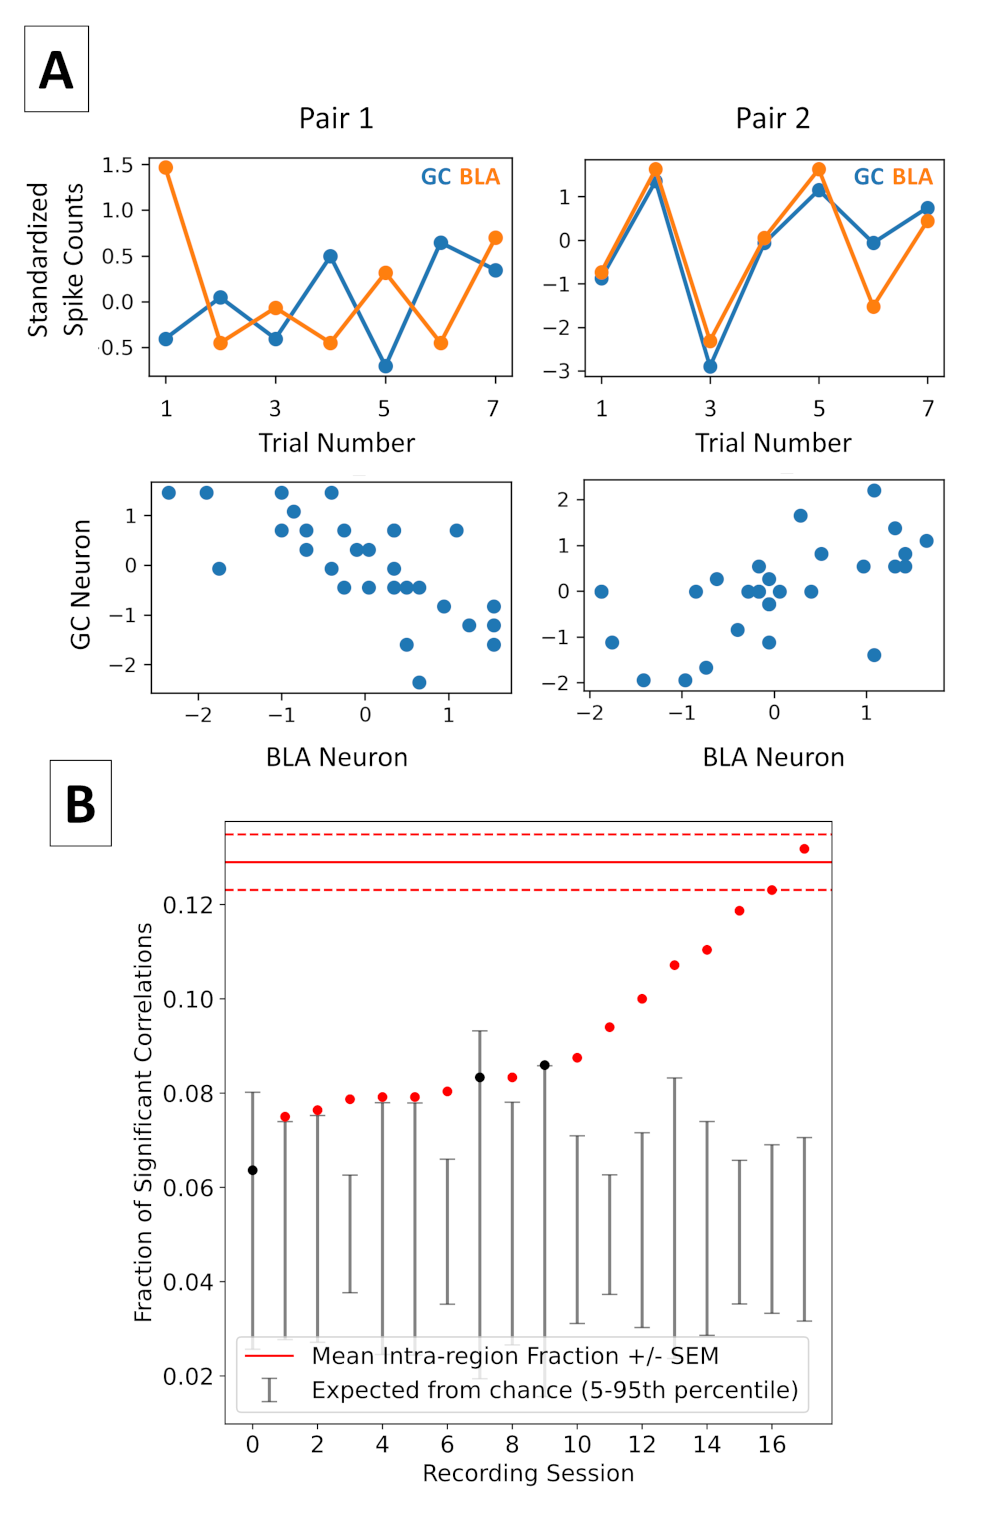
\includegraphics[width=0.5\linewidth]{mahmood_22_figures/fig6-0.png}
\caption{\textbf{BLA and GC show strong spike-count correlations on a trial-matched basis. (A)} Top row: Representative timeseries of (standardized) spike counts for two BLA-GC neuron pairs. Shown for each are consecutive sets of 7 trials (out of 30) showing negatively correlated (left) and positively correlated activity (right). Bottom row: Same data as top (but including all 30 trials) row plotted as a scatterplot showing all of the trials/pair; the negative (left) and positive (right) correlations in the scatterplot are easily seen. \textbf{(B)} A comparison of the fraction of significant correlations across all comparisons (neuron pairs x tastes) for trial-matched and trial-shuffled (i.e., GC trial 1 compared to BLA trial 4, etc) data. Trial-matched spike-count correlations (filled circles) are in all but 3/18 sessions significantly higher compared to the trial-shuffled comparisons (vertical lines); error bars show the 5-95th percentile interval of fraction of significant correlations per session expected by chance, red circles (n=15) show sessions for which the fraction was higher than expected by chance, and black circles (n=3) show sessions for which the value was within the chance interval. The interval marked by the horizontal dotted lines shows the Mean +/- SEM fraction of significant intra-region correlations (i.e., all BLA-BLA and GC-GC neuron pairs), included for reference.}
\label{fig:wrapfig}
\end{figure}

Across the entire sample, BLA-GC neuron pairs (averaged across all pairs in a single session) almost always showed higher spike-count correlations than did trial-shuffled data (Fig. 6B, 15/18 comparisons had values significantly higher than those expected by chance, n = 18 sessions from 6 animals), confirming that the taste responses of simultaneously-recorded BLA and GC single neurons are coupled in magnitude. Of course, either positive or negative correlations indicate connectivity at the single-neuron level, since a neuron pair can have either an effective excitatory or inhibitory connection between them; both connection types characterize projections connecting BLA and GC, and either can create coordinated dynamics between both regions (\cite{haley2016a,fu2020a}).

\subsection{The time-courses of BLA and GC taste responses are coupled}
The above analysis reveals a broad coordination in BLA-GC neural activity—trial-to-trial differences in firing rates in BLA neurons, measured in stimulus-evoked responses separated by >20 seconds, predict trial-to-trial differences in firing rates in simultaneously recorded GC neurons. But this result falls short of revealing whether this amygdala-cortical coupling has anything specific to do with taste processing. It is possible that taste responses are simply “riding on” generally coupled excitability existing at long time-scales, not unlike that detected in studies of “resting-state network” dynamics (\cite{raichle2015a,seitzman2019a}). Given our proposal that a central feature of BLA-GC coherence is the specific coupling of state-to-state transitions, it is important to first test whether this inter-regional coherence is epoch-specific.

\begin{figure}
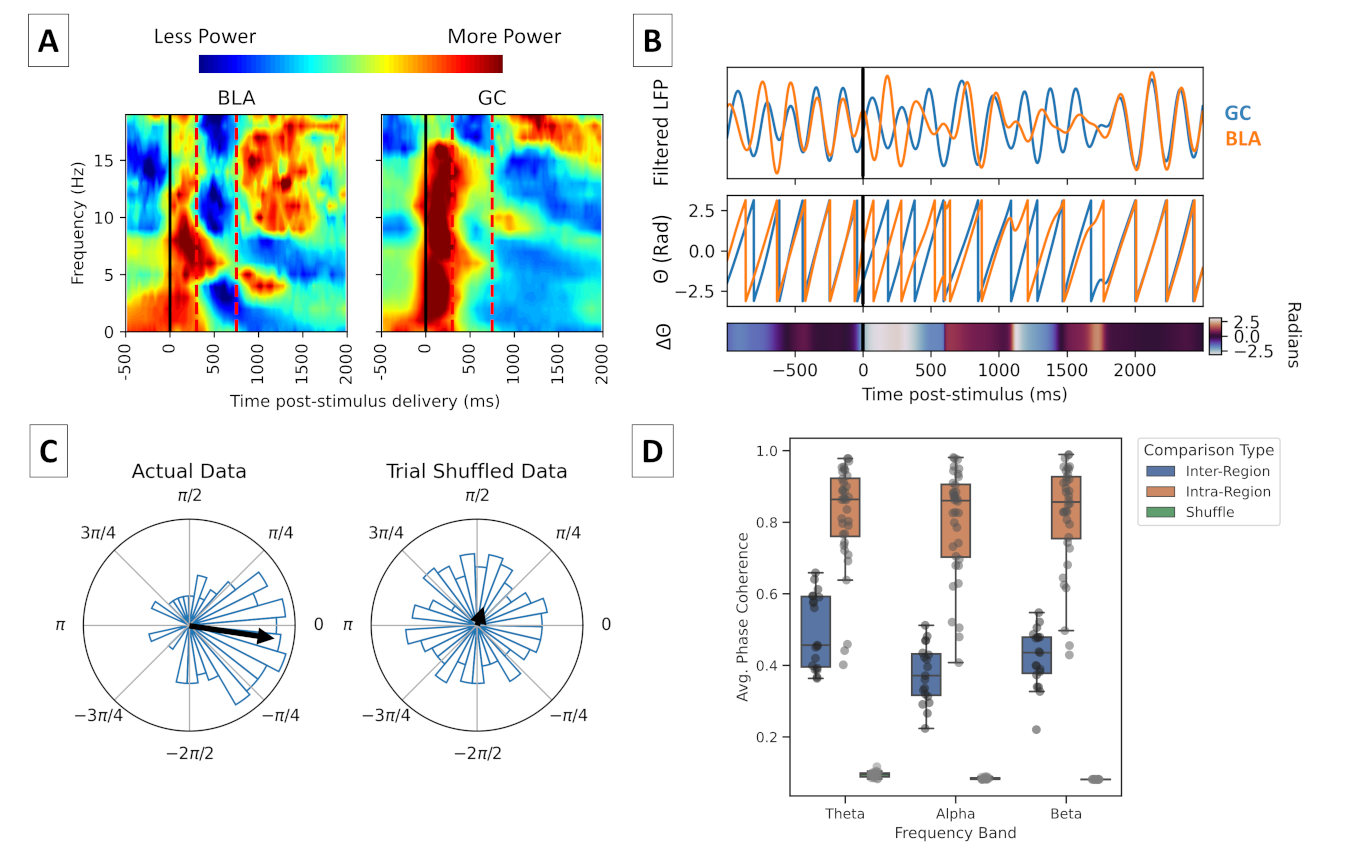
\includegraphics[width=\linewidth]{mahmood_22_figures/fig7-0.png}
\caption{\textbf{BLA and GC evoked LFP responses are similar on a trial-matched, but not trial-shuffled basis. (A)} Trial-averaged spectra of GC and BLA taste responses. Solid black lines mark taste delivery, and dashed red lines mark the average times of epoch onsets, which are well aligned with changes in the spectra in both regions. Power in each plot is Z-Scored by frequency for the time periods shown. \textbf{(B)} Calculation of BLA-GC phase difference for a single trial. Top panel shows filtered LFP (4-7 Hz) for each region, middle panel shows extracted phase (\Theta\)), bottom panel shows phase difference (\Delta\Theta\)) \textbf{(C)} Phase difference histograms (length of blue bars = frequency of occurrence) used to quantify similarity between GC and BLA LFP using average inter-trial phase coherence. Small phase differences (indicated by strong peaks in the polar histogram close to 0) indicate strong coherence. This is quantified using the magnitude of mean phase difference vector (black arrows). Data show the  distribution of phase differences for t=0ms post-stimulus delivery for actual and trial shuffled data. \textbf{(D)} Mean phase coherence for 0-2000ms post-stimulus delivery across frequency bands. The value of the trial-matched comparison is significantly higher than the trial-shuffled comparison, suggesting that there are similarities in the activity of both regions which are not present in “trial-averaged” data.}
\label{fig:wrapfig}
\end{figure}

We therefore moved next to examining coherence in the time-courses of taste-evoked responses, using analyses of local field potentials (LFPs) that have often been employed for such purposes (\cite{antzoulatos2016a,place2016a,saravani2019a}). Even casual scrutiny reveals what appear to be striking similarities in the (trial-averaged) spectral power/amplitude of BLA and GC field potentials (Fig. 7A). While the dominant frequencies differ between regions, in both regions the frequency spectra change repeatedly across the 1-1.5sec following stimulus delivery, in a manner that is well aligned with the approximate average timing of epochal transitions of ensemble firing described previously (see Fig. 2, and \cite{fontanini2009a,katz2001a,sadacca2016a}). 
These observations were statistically evaluated using quantification of the inter-trial phase coherence (\cite{stitt2017a,engel2020a,kramer2020a,zareian2020a}) between BLA and GC taste responses. Briefly, phase information for BLA and GC LFPs (across the 4-30 Hz band) was extracted using the Short Time Fourier Transform, after which phase differences between the two regions were calculated (Fig. 7B). These measurements were aggregated across all trials for each time-bin separately, and the variance was evaluated across post-stimulus time bins (see Fig. 7C); the tighter the resulting phase-difference distribution, the stronger the coupling. The results of this analysis revealed that, while inter-areal coherence (blue bars) was inevitably smaller than intra-areal coherence (tan bars), it was significantly larger than the (control) coherence between mismatched trials (Fig. 7D; it’s worth noting that this measurement likely under-estimates the true cross-coherence, because any epoch-to-epoch differences will add to the variance and reduce the across-trial average). This result held for all of the frequency bands that we assessed (theta: 4-7Hz, mu: 8-12Hz, beta: 13-25Hz, F(2,34)=654.5, p=7.21x10-28 for “Comparison Type” using Repeated Measures ANOVA; for all pairwise comparisons p=1.61x10-7 [all p-values are at the lower bound for numerical error], pairwise Mann-Whitney U Tests, n = 18 recordings across 6 animals). Qualitatively similar results were observed for simple cross-correlations between LFP power spectra for BLA and GC (data not shown). The trial-averaged time-courses of GC and BLA activity, as measured in evoked LFP activity, are coupled above and beyond overall magnitudes, in a manner that looks, at first blush, to be related to epochal processing (\cite{katz2001a,fontanini2009a,sadacca2012a}).  

\subsection{BLA and GC cross-coherence is epoch-specific}
Given the above, the fact that the different GC epochs have been shown to reflect distinct coding processes, and the likelihood that BLA is more integrally involved in the coding of palatability than taste identity (\cite{piette2012a,lin2021a}) , we hypothesized that, beyond the overall time courses being coupled, the cross-coherence between GC and BLA (evaluated in LFP time-courses) would itself be epoch-specific. 

Our test of this hypothesis is summarized in Fig. 8, which reveals that phase coherence between BLA and GC is in fact modulated in an epoch- (and, as it turns out, frequency-) specific manner by stimulus delivery. Changes in the theta (4-7Hz) band were centered largely on the initial (i.e., taste-nonspecific) epoch of the responses: in most (11/18) sessions, \(\theta\) activity changed significantly from baseline; overwhelmingly (in 9/11 cases), these early-response changes involved a decrease in phase coherence. In the mu (7-11Hz) band, meanwhile, changes were centered on the later (palatability-specific, see \cite{katz2001a,sadacca2012a}) response epoch; these changes, which were even more ubiquitous than \(\theta\) changes, in every case involved a decrease in coherence (see the right-hand panels of Fig. 8A-B, n = 18 recordings across 6 animals). A reduction in coherence following stimulus delivery was predictable given previous results showing that strong levels of inter-region coherence tend to be associated with states of “low cognitive engagement” such as sedation, epilepsy, and cognitive impairment (\cite{supp2011a,martinet2017a,arbab2018a}), as well as the fact that BLA and GC “encode” tastes non-identically – hence, their specific neural responses are likely to differ (see also Discussion). Note, however, that phase coherence always stays higher than random levels (BLA and GC are never functionally “disconnected”), and that state-specific reductions in coherence can be recapitulated in simple, tightly interconnected model networks (see below). 

\begin{figure}
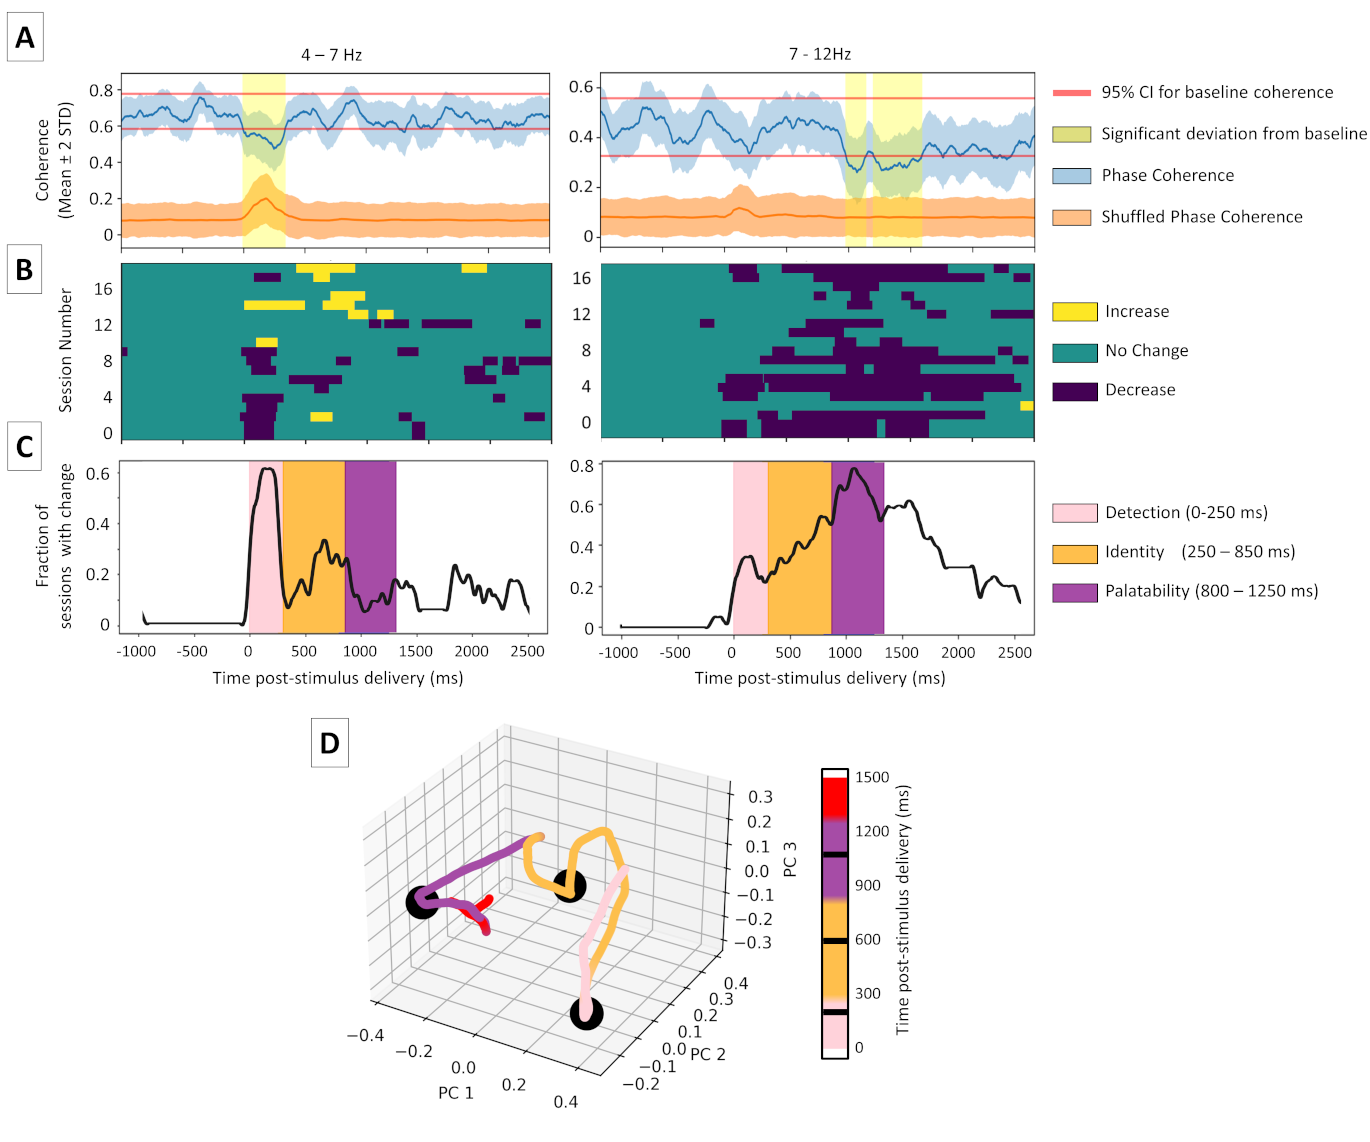
\includegraphics[width=\linewidth]{mahmood_22_figures/fig8-0.png}
\caption{\textbf{BLA-GC LFP phase coherence shows epoch-locked dynamics. (A)} Representative examples of phase coherence in the 4-7 Hz \(\Theta\), left) and 7-12 Hz \(\mu\), right) bands. Red lines denote the 95\% confidence intervals determined by baseline coherence (-750 to -250 ms relative to stimulus delivery), and the yellow shading marks timepoints at which mean coherence changed significantly from that baseline. \textbf{(B)} Timepoints and directionality of changes in phase coherence relative to baseline for all sessions. While changes in the 4-7 Hz band show both increases and decreases (note that the most prominent changes from baseline, which are found in the earliest aspects of the responses, mostly consist of reductions of coherence), changes in the 7-12 Hz band consist entirely of decreases in coherence. \textbf{(C)} The fraction of recordings in which phase coherence deviated from baseline. Bands correspond to those of the plots above them. Note that the timepoints of changes in coherence relative to baseline match strongly with timings of the “canonical” taste epochs (noted with overlain shading). \textbf{(D)} PCA projection of changes in phase coherence (as in panel C) for 4-100Hz. Black circles indicate “corners” in the trajectory, the timings of which roughly correspond to each epoch (black ticks marks in colorbar). Colors indicate durations of epochs as in (C).}
\label{fig:wrapfig}
\end{figure}

To aggregate these results across the entire dataset, we calculated the fraction of recordings in which coherence diverged significantly from baseline at each time point across the evoked response (Fig. 8C). These results confirmed the representativeness of the examples above, showing that 4-7Hz coherence tends to be modulated early in the response, and that 7-12Hz coherence modulation comes on later in the response. While we have no specific explanation for why “theta” coherence highlights an earlier epoch and “mu” a different epoch, what is clear is that phase coherence illuminates the fact that BLA-GC coupling is modulated by epoch, as predicted.

To further illustrate the epoch-specificity of BLA-GC functional connectivity, we subjected deviations of coherence from baseline across a broad range of frequency ranges (4-7, 7-12, 12-30, 30-70, and 70-100Hz) to dimensionality reduction. In all bands we observed decrements in coherence, albeit with distinct temporal profiles (data for higher bands not shown). When we projected these timeseries of coherence deviation onto 3 principal components (Fig. 8D), the epoch-specific nature of BLA-GC coupling came into focus: the timing of sudden “turning points” in the trajectory, which are highlighted in Fig. 8D using black circles, roughly correspond to the center points of the canonical epochs. Collectively, these data strongly recapitulate the epoch-wise nature of taste processing that has been recognized in GC and BLA spiking data, demonstrating that BLA-GC functional connectivity is not static, and that BLA activity is explicitly tied to previously-described GC dynamics (\cite{lin2021a}).

\subsection{BLA and GC ensembles undergo coupled state transitions}
The structured dynamics of BLA-GC phase coherence suggests not only that BLA and GC population activity is coordinated, but that this coordination is modulated according to the unfolding taste response. It further suggests that the trial-to-trial variability in amygdala-cortical dynamics might be coupled, providing indirect evidence for our riskiest hypothesis—that the sudden, behaviorally-relevant transitions between ensemble firing-rate states (transitions that are a reliable facet of GC ensemble taste activity and that occur at different latencies in different trials) might be a distributed network phenomenon, coupled across GC-BLA ensembles. Such nonlinear coupling would suggest that BLA and GC behave as a distributed, yet single (putatively attractor) network, processing tastes in a unified manner in real-time.

The analyses described in the above sections fall short of truly testing this hypothesis. In fact, they are strictly limited in their interpretability in this regard, specifically because population spiking changes in GC are quite sudden and the latencies of these transitions vary by hundreds of milliseconds from trial to trial (\cite{jones2006a,sadacca2016a}); these two properties of ensemble transitions ensure that any ability to evaluate their coupling will be essentially lost in across-trial averaging and obscured in moving-window analyses. Only through direct, single-trial analyses of the transitions themselves can we hope to evaluate BLA-GC coupling of such phenomena. 

\begin{figure}
\centering
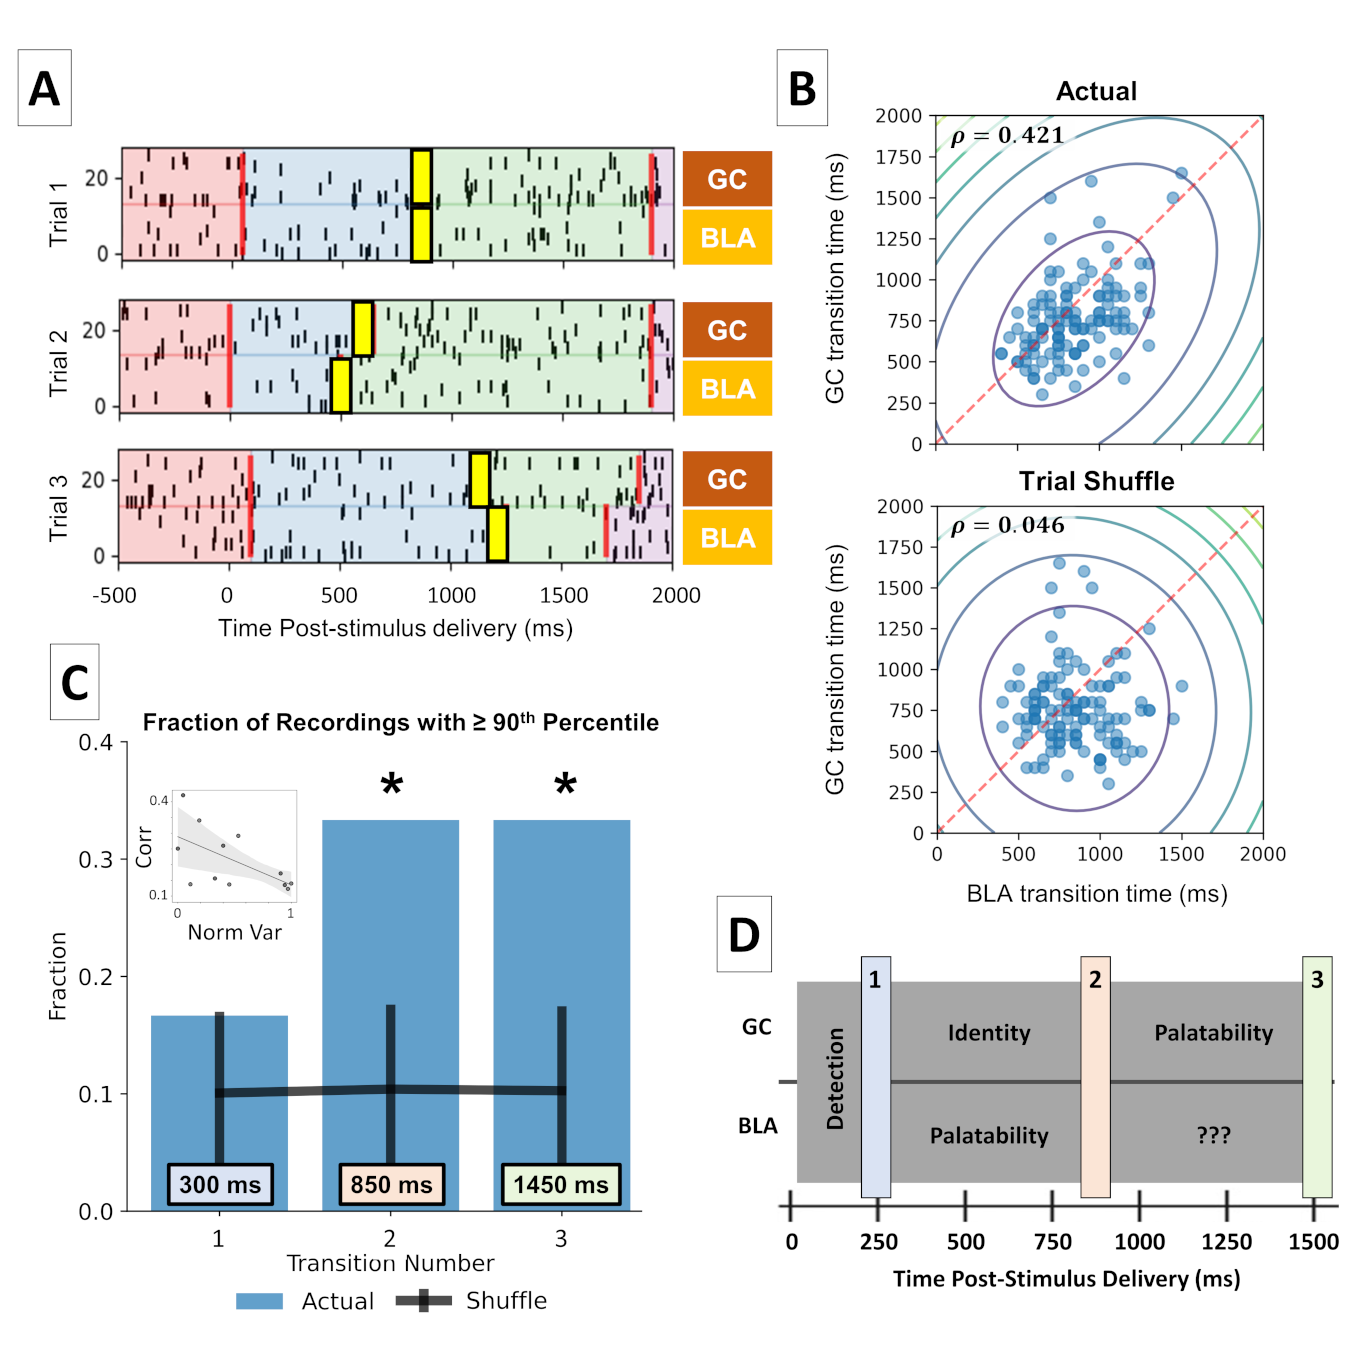
\includegraphics[width=0.9\linewidth]{mahmood_22_figures/fig9-0.png}
\caption{\textbf{BLA and GC population evoked responses involve coordinated state transitions. (A)} Three representative trials highlighting the co-variance of Transition 2 between BLA and GC. Transition 2 is highlighted with thick yellow lines. \textbf{(B)} The inferred times of GC state transitions plotted against those inferred for the simultaneously recorded BLA population for each trial of a representative transition; the scatterplot is overlain with contours of a 2D gaussian around the data cloud. The top plot shows actual data; the bottom, trial-shuffled data. ρ = Spearman’s Correlation Coefficient \textbf{(C)} The fraction of datasets showing significant correlations for each transition (* : p<0.05). Blue bars represent the value in the actual data, and black lines indicate mean ± STD for fraction expected from random data. Only the fraction for Transitions 2 and 3 reached statistical significance. Colored boxes show average latency for each transition (post-stimulus delivery). \underline{Inset}: The variance (uncertainty) of transition latency distribution is significantly related to the correlation strength between BLA and GC transitions. Scatterplot shows correlation strength vs. normalized variance of inferred transition posterior distribution \textbf{(D)} The timings of the inferred transitions matches well with the canonical epoch-onset times. Transitions 2 and 3 bookend the palatability epoch in GC (figure adapted from Fontanini et al., 2009).}
\label{fig:wrapfig}
\end{figure}

Given the novelty of this direct examination of inter-regional correlation of transition times, we first performed pilot analyses in which we divided datasets of simultaneously-recorded GC neurons into halves, separately applied changepoint inference to each half-population, and correlated the latency of each transition between the two fits. We observed statistically significant correlations for >80\% of our datasets and for each transition (n=11 recordings; data not shown), confirming that our correlation measure is a robust metric for determining transition coupling between ensembles (note that even these correlations were not significant for all datasets, and did not reach rho=1.0 for reasons discussed below, also see Methods). 
We then brought this analysis to bear on simultaneously recorded BLA and GC ensembles, independently estimating transition times in each, and then testing whether the latency of the 1st GC transition was correlated with the latency of the 1st BLA transition, etc. The results of this test, which are summarized in Fig. 9, demonstrate that certain transition times in BLA and GC ensembles are indeed robustly coordinated. Fig. 9A presents one representative set of spike-trains, showing inferred changepoints for a pair of simultaneously-recorded BLA and GC ensembles, and clearly revealing the close apposition of these transitions. Fig. 9B (top panel) shows a scatterplot of independently calculated latencies of the 2nd transition (the behaviorally-relevant transition into palatability-related firing in GC; \cite{sadacca2016a,mukherjee2019a}) from each of the trials for a representative session; the bottom panel of Fig. 9B shows the scatterplot that would be expected by chance (produced after randomly shuffling a set of changepoint latencies between trials for the same dataset). The significant covariance between the GC and BLA changepoints in the top panels is lost with trial-shuffling, proving that this transition alignment between the two regions is a within-trial phenomenon.

We statistically evaluated the strength of this BLA-GC transition coupling across the entire dataset by calculating the fraction of transitions that exceeded the 90th percentile of correlation strength relative to their respective trial-shuffled correlations (“strongly correlated” transitions), and statistically comparing this number to the fraction of strong correlations expected by chance for a similar sized dataset. This analysis revealed that the fraction of strongly correlated BLA and GC transition times in our data were significantly higher than those expected by chance, but only for the transitions into and out of the GC palatability-related state (Fig 9C; Percentiles=99.56 and 99.64, p=4.05x10-3 and 3.65 x10-3 for transitions 2 and 3 respectively, Bonferroni-corrected alpha=0.05/3=16.67x10-3, Shuffle test with Bonferroni’s correction, n = 18 recordings across 6 animals, see Methods). 

Note that this evidence of significant coupling—the fact that the cloud of dots in the top panel of Fig. 9B is elongated—is observed despite the relatively small ensembles of BLA neurons isolable in awake rats. It is quite likely that a good deal of the noise visible in this panel reflects unavoidable noise in the estimation of transition time (see Methods). To test this suspicion, we calculated the relationship between the amount of uncertainty in the model’s estimation of transition time (i.e., the summed average variance of inferred transition distributions) and the strength of correlation between GC-BLA transitions. As suspected, we found a significantly negative relationship between the two variables (Fig. 9C inset; slope=-2.3, r-squared=0.352, p=0.021, One-tailed Wald Test for regression slope), a result consistent with the suggestion that uncertainty in the inference “blurs” the correlation between transitions. The strength of coordination between BLA and GC transitions is, thus, likely even stronger than that estimated here.

Note, however, that only transitions in and out of the state that has been previously shown to be related to the reaching of consumption decisions (\cite{sadacca2016a}), i.e. transitions that signaled the onset and offset of the “palatability” state in GC (schematic shown in Fig. 9D), were coupled across the BLA-GC network; transitions from the GC Detection state into GC Identity states were not. This result dovetails nicely both with classic thinking about the specific role of BLA in emotional processing (Yamamoto, 2008; Baxter and Croxson, 2012) and with recent work from the lab which shows that optogenetic perturbation of the BLA->GC projection primarily affects GC processing during the palatability epoch in GC (\cite{lin2021a}). While BLA activity during the late epoch (“???” in Fig. 9D) has hitherto not been explored, the strong BLA-GC coupling during that time period recommends further investigation into processing performed by BLA during that time period. Together, these results suggest that the “role” of BLA-GC communication likely changes between epochs, and even may only be important during the GC palatability epoch.

\subsection{Modelling coupled state-transitions with state-specific coherence}
Together, the above results fill in a picture of BLA and GC as processing tastes as a single distributed unit, with significant (above-chance) cross-coherence punctuated by coupled state transitions across which the coherence drops in certain frequency ranges (a change indicative of intense processing). From a dynamical systems perspective, this phenomenology makes sense: “instantaneous” coherence will often be state-specific within a system in which state transitions are synchronized across brain regions; for just one example, brain regions collectively transition between different states of sleep; \cite{stitt2017a}. We would argue, in fact, that it is common for distributed networks of interconnected neurons to perform coupled transitions between states, some of which demonstrate decreases in LFP phase coherence.

\begin{figure}
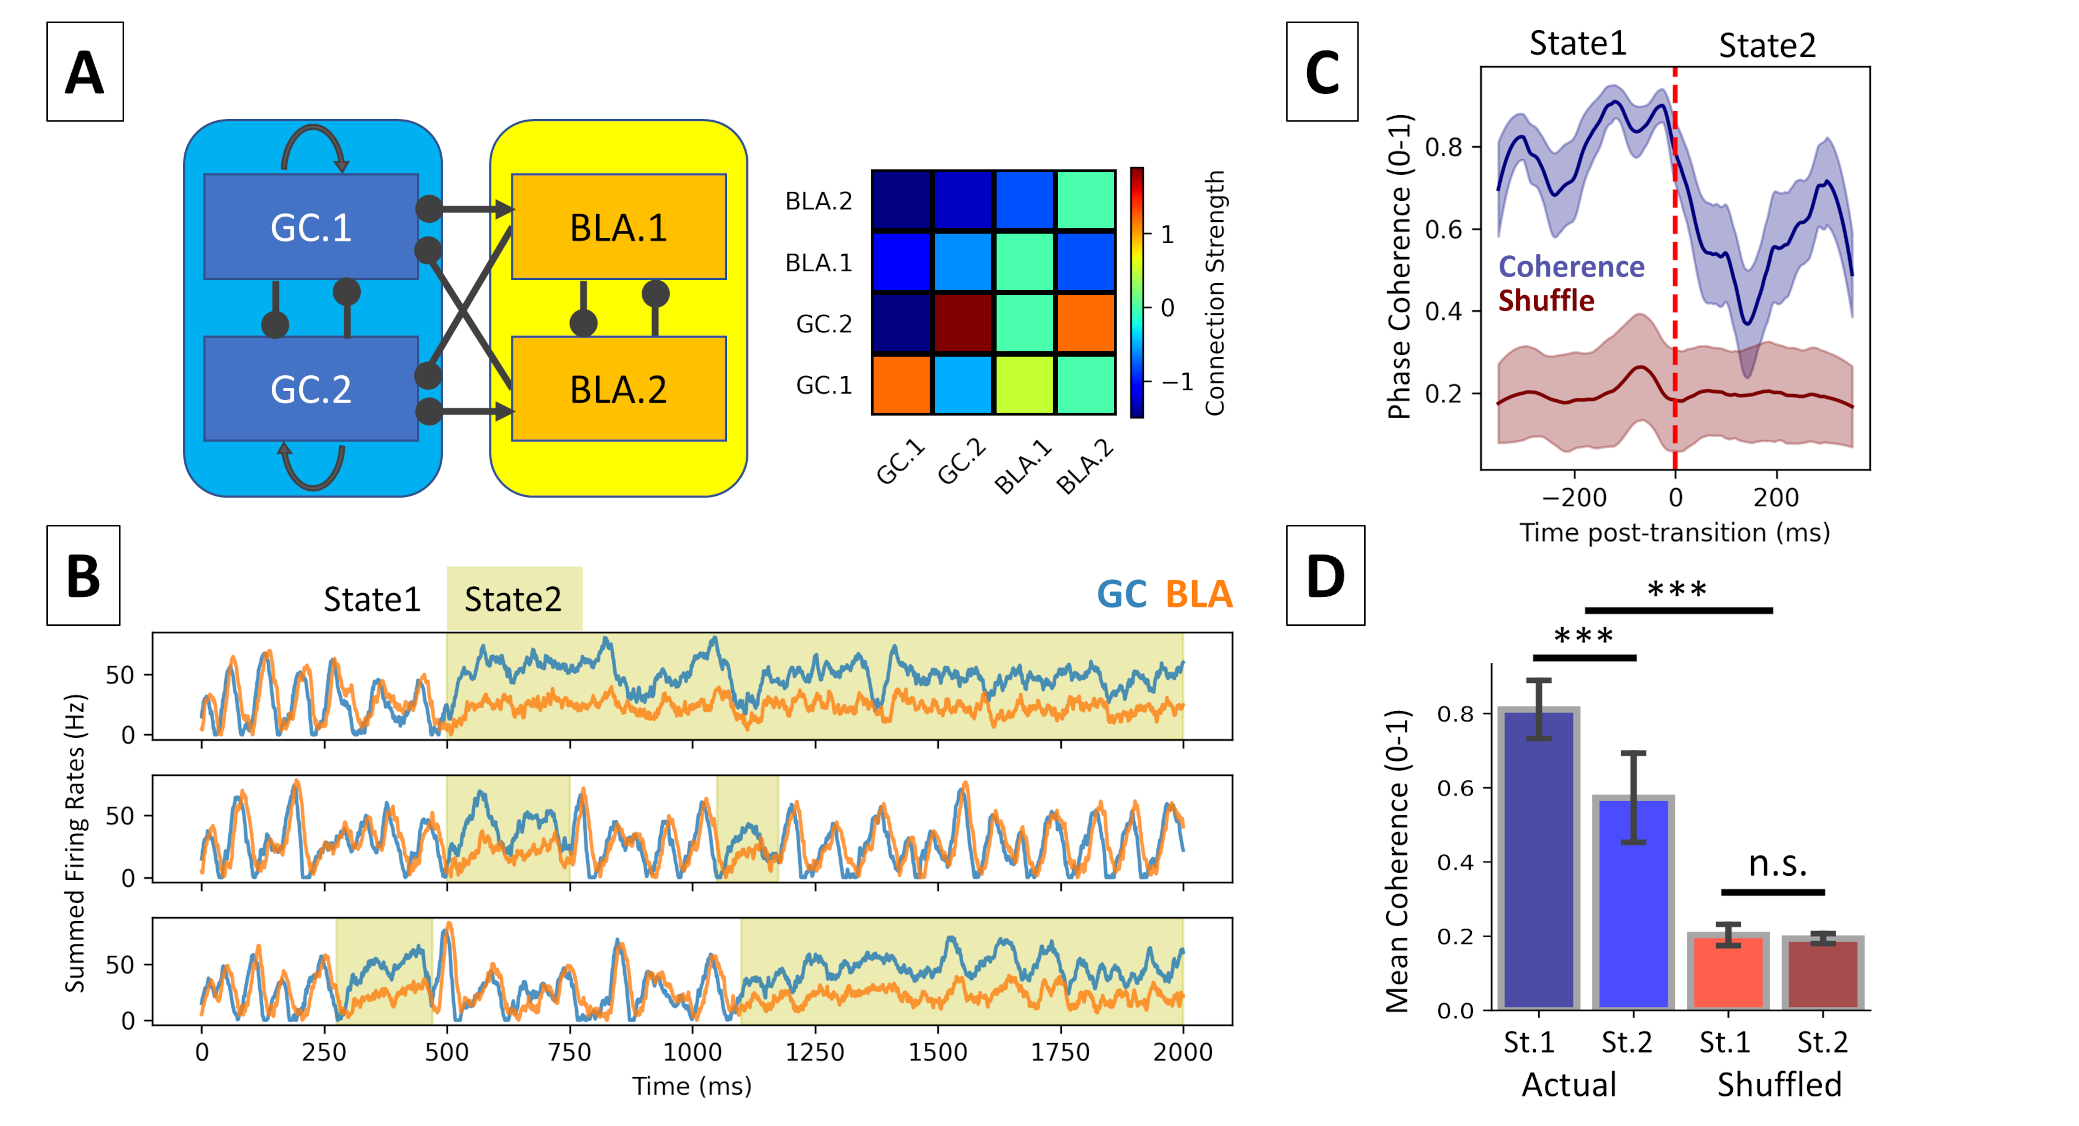
\includegraphics[width=\linewidth]{mahmood_22_figures/fig10-0.png}
\caption{\textbf{Coordinated state transitions and state-specific coherence in a coupled network model. (A)} Network of 4 inter-connected "subpopulations" which represent parts of GC and BLA \textbf{(B)} Example "trials" showing activity of the network. Activity from both units in each region is summed as an analog of LFP. Highlighted regions marks time periods the system spends in the less coherent state (State 2). Note that both states have finite durations. \textbf{(C)} Inter-trial phase coherence calculated on time windows 350ms before and after transition from State 1  State 2 (moreless coherent state; mean ± std). \textbf{(D)} Average coherence during each state (mean ± std; St.1 = State 1, St.2 = State 2, *** = p<0.001).}
\label{fig:wrapfig}
\end{figure}

We tested this contention by constructing a simple network model. Briefly, the network was comprised of firing-rate units which can be taken to roughly represent interconnected subpopulations of BLA and GC neurons (Fig. 10A; the right panel shows the connection strengths between subpopulations). When challenged with a moderate amount of input delivered to both “regions” (simulating either noise or taste stimulation, which initially arrives at BLA and GC via distinct paths; see \cite{gal-ben-ari2012a}, the network enters a mode in which it switches between a “more coherent” state characterized by strong oscillations, and a “less coherent” state where clear oscillations are disrupted (a switch that necessarily changes functional connectivity). Fig. 10B presents the summed firing rates of simulated BLA and GC units across 3 “trials,” in which the network can be seen to collectively transition between the states, one of which is clearly endowed with higher cross-coherence (State 1) than the other (State 2).
Fig. 10C provides a specific analysis of these appearances, revealing that coherence indeed decreases following the transition into the less oscillatory state (State 2). In neither state, however, does this cross-coherence decline to baseline levels—the populations never fully disconnect (Fig 10C and 10D, 2-Way ANOVA with State and Dataset [Actual vs Shuffle] as factors, State : F(1) = 184, p=0.001; Dataset : F(3) = 184, p=0.001; State*Dataset : F(3) = 233, p=0.001; Tukey’s HSD post-hoc tests, Actual St.1 vs St.2 : T = 42.7, p = 0.001; Shuffle St.1 vs St.2 : T = 1.74, p = 0.302). And while this network is admittedly simple (a fact that no doubt explains the simple, randomly-timed "back and forth" between two states), it is not the only way that such a model can be constructed: other versions can allow each region to intrinsically oscillate at different resonant frequencies, for instance, where such frequencies would inevitably be expressed to differing degrees in different states. The important point is that this variant of the model would, like many such variants (and the real networks recorded for this study), progress through state transitions in a unified manner, and that phase coherence would be lower following certain transitions. While our investigation of the model is limited to recapitulating the state-specific changes in coherence we see in our data, this recapitulation further highlights the aptness of such “attractor models” for explaining activity in GC and BLA, and therefore being good candidates for theoretical investigation to generate predictions about the system to be tested in future experimental work (also see Discussion).

Ultimately, these simulations demonstrate that a multi-region network can undergo collective, coupled state transitions while having variable functional connectivity during each state. We suggest that the amygdala-cortical system is just such a network.

\section{Discussion}
Much of the research that has explored how brain regions work together (\cite{markov2014a,grabska-barwi2017a,yates2017a,glaser2018a}) makes two broad assumptions: 1) neural responses are identical (save for noise) across repeated stimulus presentations; and 2) neural dynamics evolve on slow timescales (hundreds of milliseconds, or even seconds). These assumptions fail in many cases (\cite{gat1997a,sugase1999a,latimer2015a,jones2007a}), including the present study. In such cases, examination of coupling requires methodologies that can parse sharper changes in neural activity and account for trial-to-trial variability.

In the context of taste processing, gustatory cortex (GC) and basolateral amygdala (BLA) form strong candidates for coupling. Both are involved in driving taste-related behavior—perturbations of either results in similar behavioral changes (\cite{lovaglio2010a,lin2011a,lin2018a}), perturbation of BLA changes GC response dynamics (\cite{piette2012a}), and BLA-GC connectivity is important for taste learning (Lin and Reilly, 2012). Furthermore, taste-evoked activity of single-neurons in the two structures (\cite{fontanini2009a,sadacca2012a}) undergoes changes (and encoded information) at the same time points. 

These facts motivate the current study but stop short of actually testing the hypothesis that BLA and GC transition synchronously. Hitherto, the most direct test of BLA-GC coupling has involved acute optogenetic perturbations of BLA->GC axonal projections (\cite{lin2021a}). This perturbation decreased GC ensemble coherence during the transition to palatability coding, and reduced palatability-relatedness of single-neuron firing following this transition. Brief, bilateral optogenetic perturbation of GC neurons themselves, meanwhile, delivered before or during this transition to palatability coding (\cite{mukherjee2019a}), delayed the gaping response of rats to bitter quinine until after the perturbation was removed; hence, while this GC perturbation hindered planning and execution of the taste motor response, it is likely that the remainder of the circuit maintained output-relevant information, enabling a rebound from the perturbation. 

Results of the above studies—the fact that some palatability-related information in GC survives silencing of BLA->GC axons, and the fact that gaping quickly recovers after GC perturbation—in conjunction with the results from the current study, suggest that while BLA and GC are strongly coordinated, they are only parts of an even larger network. This conclusion is further bolstered by work showing: 1) that other brain regions show response dynamics similar to BLA and GC (lateral hypothalamus : \cite{li2013a}; and parabrachial nucleus of the pons : \cite{baez-santiago2016a}); and 2) that while palatability responses in GC show a gradient of hedonic values, those in BLA are largely binary (good vs. bad, \cite{fontanini2009a,sadacca2012a}). Clearly, there are additional regions (perhaps the lateral hypothalamus) that process palatability information in parallel to BLA to produce the more nuanced coding seen in GC. 

In this context, our results are also consistent with those showing that distributed nodes in tightly-coupled systems can produce non-identical coding during stimulus processing, and encode “redundant” information to varying degrees (\cite{siegel2015a,brincat2018a,lara2018a,saravani2019a}). This is not truly surprising: complex systems tend to couple on multiple time-scales; just as one unit of such a system might increase its spiking while another is silent, and vice-versa (Fig. 6A), one’s firing might reflect palatability at one time point, and then the other do so afterward. The fact that palatability-relatedness moves from BLA to GC might simply reflect a single cycle of an oscillation.

The advance offered in this study has to do with the subtlety of the predicted coupling, which rendered previously-used methodologies for investigating that coupling insufficient. Specifically, we predicted that (trial-specific) moments of ensemble state transitions in GC and BLA would be synchronized. This hypothesis could not be tested using analyses that fail to account for dynamics of functional connectivity, collapse data over large time-scales (e.g. whole trials), or assume that all trials are dynamically identical. In the current context, such analyses provide misleading information: both the spike-count correlation and the LFP-phase coherence analyses show BLA and GC to be significantly coordinated but fail to give us any information about temporal dynamics; meanwhile, changes in BLA-GC inter-trial phase coherence (which is de rigeur for characterizing inter-regional coupling, see \cite{engel2020a,kramer2020a,zareian2020a,zielinski2019a}) reveal only state-specific reductions in coupling (Fig. 8).

Such state-specific changes in coherence have been seen in transitions between sleep states (\cite{stitt2017a}), and between attentive and inattentive states (\cite{siegel2008a}). While the states in evoked activity described in this paper are more fleeting than the much longer brain states studied by \cite{stitt2017a,siegel2008a}, in each case changes in phase coherence mark changes in brain states. Specifically, reductions in coherence such as we observe here have been shown to be associated with intense processing (\cite{supp2011a}), whereas increases in coherence are associated with cognitive impairments (\cite{martinet2017a,arbab2018a}). Such low correlations in activity are entirely compatible with strong coupling (\cite{schneidman2006a}). Particularly given the fact that BLA-GC phase coherence always stays well above chance levels, it is safe to say that this observation of decreased coherence does not mean that GC and BLA are becoming “decoupled” at any time point. 

Again, had we stopped our analysis at phase coherence, we would have reached the wrong conclusion about amygdala-cortical coupling during taste processing; only the novel transition coordination analysis (which accounts for both dynamics over the course of the trial and variability across the trials) allowed us to directly test the risky hypothesis that taste processing is characterized by sudden ensemble state transitions shared across BLA and GC. Our successful test of this hypothesis strongly corroborates the results of causal studies showing that wholesale inhibition of BLA (\cite{piette2012a}) and precise perturbation of the BLA->GC axonal projection (\cite{lin2021a}) specifically perturb processing during—and the transition to—the palatability-related (late) epoch of GC taste coding. This further underscores the limitations of more canonical communication measures with regard to the theories that they are able to test, and provides further evidence for the dynamic nature of the BLA-GC interaction.

Together, these results suggest that taste responses observed in BLA and GC are poorly described by feedforward/hierarchical (\cite{parras2017a,glaser2018a,heidari-gorji2021a}) models, and better described as working in a joint fashion. Our finding of coordinated state-transitions is appealingly (if speculatively) explained in terms of collective attractor states (\cite{miller2010a,litwin-kumar2012a,camera2019a,recanatesi2022a}). Such models require strong, bidirectional connectivity that is observed throughout the taste circuit (Bielavska and Roldan, 1996; McDonald, 1998; Shi and Cassell, 1998), and predict/recapitulate the sharp state transitions that have been reported in GC (\cite{jones2007a,sadacca2016a}), BLA (this study), and other brain regions (\cite{seidemann1996a,gat1997a,sugase1999a,latimer2015a}). Another attractive aspect of such a theory is the fact that “noise”, rather than being a nuisance variable, serves as the force driving state transitions, allowing robust performance in noisy conditions (\cite{miller2013a}) and explaining the large variability observed in evoked neural and behavioral responses on a trial-by-trial basis (\cite{kisley1999a,carandini2004a,jones2007a,kotekal2020a,peixoto2021a}). Given the ubiquity of “noise” in biological systems (\cite{shadlen1994a,shadlen1998a,miller2010a}), it seems likely that valid mechanisms of function will be those that have this property. 

Of course, causal confirmation of this theory waits upon evidence that the two structures influence one another recurrently— i.e. studies investigating the role of the GC->BLA (“reverse”) projection in taste processing. While the GC->BLA projection has been shown to be important for taste-related learning, (\cite{lavi2018a,kayyal2019a}), it’s role in generating passive taste responses is yet to be elucidated. If recurrent circuitry plays a role in taste processing, perturbation of the GC->BLA projection should change not only activity in BLA but also the “source” activity in GC, reflecting the fact that the circuit processes information in a loop fashion. Such an outcome would further drive home the value of moving away from “feedforward” biases in the study of taste processing. 

Ultimately, a nuanced understanding of inter-region communication, and of how this communication is important for generating behavioral output, will require that we appreciate the sorts of nonlinearities and variability examined here—that we do not smooth out potentially important sudden ensemble changes in real-time ensemble activity. The current study furthers our trial-specific understanding of neural activity and will hopefully drive further questions regarding the role of reciprocal connectivity and meta-stable dynamics in sensory processing.

\printbibliography[title={References}]

\end{refsection}
\begin{refsection}

\chapter[Dynamic Function of Neurons]{The function of groups of neurons changes from moment to moment}

Chapter 4 is a reproduction of an article published as:\\\\
Lin, Jian-You, et al. “The Function of Groups of Neurons Changes from Moment to Moment.” Current Opinion in Physiology, vol. 20, Apr. 2021, pp. 1–7. ScienceDirect, https://doi.org/10.1016/j.cophys.2020.12.002.

\section{Abstract}
Modern techniques that enable identification and targeted manipulation of neuron groups are frequently used to bolster theories that attribute specific behavioral functions to specific neuron types. These same techniques can also be used, however, to highlight limitations of such attribution, and to develop the argument that the question ‘what is the function of these neurons?’ is ill-posed in the absence of temporal and network constraints. Here we do this by first reviewing evidence that neural responses are dynamic at multiple time scales, making the point that such changes in firing rates imply changes in what the neuron is doing. Studies involving brief perturbations of neural populations confirm this point, showing that the functions in which these populations participate change across seconds and even milliseconds. Based on these studies, we suggest that it is inappropriate to assign function to sets of neurons without contextualizing that assignment to specific times and network conditions.

\section{Introduction}
The increasing availability of sophisticated molecular biological techniques affords neuroscientists new means of interrogating the function of specific neurons and neuron groups. It has become commonplace to track the identity of neurons that are active as an animal performs a behavior, and to silence genetically identified (or pathway-specific) sets of neurons in the context of recording/imaging/behavioral experiments. The nature of these techniques is such that when experimenters make performance worse by silencing a set of neurons, the experimenters inevitably conclude that they have uncovered the function (or at least a function) of that set of neurons; null results are interpreted as evidence that the neurons responsible for that function have yet to be isolated. The development and use of these techniques synergizes with the popularity of theories in which function is ascribed to identifiable cell groups, both testing and driving such theories.

This approach has been remarkably successful, in that the recent literature is rife with articles enumerating the involvement of specific cell types in specific neural or behavioral functions (\cite{adamantidis2015a,balthazart2020a,biselli2019a,janak2015a,tye2012a}). It is worth noting, however, that while these modern techniques allow the experimenter to directly assay or manipulate the firing of a single cell type, observing a significant decrement in some behavioral measure as a result of silencing one set of neurons does not necessarily imply that the set of neurons in question is uniquely involved in the function under study. As just one general example, results showing that silencing projection neurons has one effect whereas silencing inhibitory interneurons has the opposite effect may not imply different specific functions for those two neuron types, but rather a wholistic function of a network of interconnected neurons that is perturbed in opposite directions by manipulations that impact overall network excitability in opposing ways.

But the fecundity of neural interconnections does not just mean that function within circuits is almost necessarily distributed among multiple cell types. These interconnections also motivate an argument that the entire research endeavor should be reconsidered --- that the very act of mapping function (or at least behavioral function) onto cell types ignores the complex dynamics of neural ensemble responses, and that ascribing specific functions to specific neurons is unwarranted. This is the argument that we unpack here: we start with evidence that the multi-scale firing dynamics --- firing-rate dynamics that are part and parcel of the activity of neurons embedded within networks --- means that function changes across learning, across changes in context, and even across parts of seconds. We go on to show that the impact of perturbing the activity of neural ensembles differs depending on the timing of the disruption, and that even two identically timed perturbations may have different impacts (because firing-rate dynamics do not necessarily unfold at the same rates in all trials). These data reveal that the functions of neurons can change dramatically over even very short spans of time, and motivate our conclusion that function is only properly assigned to groups of neurons when those neurons are placed in specific times and specific network conditions.

\section{Forebrain neural activity is intrinsically dynamic}
Most theories that ascribe particular functions to specific neurons use single numbers --- average firing-rate magnitudes --- to characterize those neurons’ responses. Neurons are classically said to ‘code’ a sensory stimulus if the average number of spikes that they fire (across a reasonable interval) in response to that stimulus significantly exceeds their spontaneous firing rate; each neuron is simply characterized as either responding significantly or not, or as having fired more or less than to other stimuli (analogous arguments can be made regarding activity related to movement, of course). Thus, it makes sense to conceptualize that neuron’s involvement in processing the stimulus in an equally simple way (\cite{chen2011a,hubel1995a,lavi2018a,mazurek2014a,steinmetz2019a,wang2018a}) --- for example, saying that a neuron that responds to sucrose, or that responds more to sucrose than to other tastes, functions to code sucrose.

If function can be attributed to a neuron on the basis of response magnitude, however, then by the same logic, changes in function can be attributed to changes in response magnitudes --- a fact that complicates attempts at simple conceptualizations of function. The truth of this logic is visible in studies of learning in the brain, and more specifically in the common (if seldom explicitly articulated) recognition that learning-related changes in neural firing represent the assumption of a new function by that neuron (that of driving learned behavior [\cite{banerjee2020a,barsy2020a,ross2018a}]). For just one classic example, consider a deep cerebellar nucleus neuron that has become responsive to a tone in a conditioned eye blink learning experiment; this neuron can be said to have acquired the function of driving an eyeblink (\cite{mm2017a}).

More recent examples make use of the very same molecular/genetic techniques that have reinforced simple theorizing about the function of neuron groups (\cite{aqrabawi2020a,butler2020a,josselyn2018a,josselyn2020a,sun2020a}). Notable among this recent work are studies showing that activation of a group of context-responsive hippocampal dentate gyrus neurons causes mice to freeze (presumably in fright) after successful fear conditioning; before the completion of conditioning, activation of these neurons does not induce freezing (\cite{ramirez2013a}). Analogously, extinguishing the prior-acquired fear memory also changes the response properties of a specific set of neurons in amygdala. Reactivation of these ‘extinction-responding’ cells comes to facilitate fear extinction behavior following learning, but does not do so before (\cite{zhang2020a}). These results drive home the point that when learning-relevant experiences change the responses of small groups of neurons, the functions in which these neurons participate change (e.g., come to drive or antagonize fear response).

But neural responses are not only plastic with learning. A growing body of evidence attests to the fact that neural responses can readily shift with changes in experimental context --- that recent experience and the understanding of the regularities of the stimulus environment (non-randomness of what stimuli appear and when) can modulate the specific properties of neural and behavioral responses to input stimuli (\cite{flores2018a,noudoost2017a}), as can the current state of the networks into which the neurons are embedded (\cite{sakata2016a}) or connected (\cite{mante2013a,safaai2015a}). Furthermore, a sensory neuron’s response may mean different things to downstream neurons in different contexts: in drosophila, for instance, the responses of looming-responsive neurons (neurons that respond to visual stimulus expansion) have distinct implications depending upon the fly’s flight status; activation of these neurons during flight instigates landing behavior, whereas activation with visual stimuli while ‘grounded’ activates different motor programs (\cite{ache2019a}). Note that while the function to which these neurons’ activity contributes depends on the stimulus (and activity driven by said stimulus), it depends with equal importance on the animal’s current state; context alters both the sensory neuron’s response and the use of that neuron’s response. This result is echoed in recent work demonstrating that the central circuit involved in processing olfactory input depends on behavioral context: taste cortex has proven to be integrally involved in olfaction, but only when the rodent is feeding, not when it is inhaling (\cite{blankenship2019a}).

The above work reveals that neurons’ responses following stimulus presentation (or, for that matter, before behavior) may change according to variables that themselves change on sub second time scales. An implication is that neural responses may undergo significant and meaningful changes across very short time periods. Recent evidence confirms this, demonstrating that single neural responses may actually be made up of multiple distinct firing rate ‘epochs’, with sequences of firing-rate changes unfolding across tens to hundreds of milliseconds (\cite{guo2015a,sauerbrei2020a,sugase1999a}). A relevant example comes from work on gustatory (taste) coding, which has this dynamic property at most central relays (\cite{baez-santiago2016a,fontanini2008a,li2016a,li2013a}): cortical single-neuron taste responses, for instance, actually involve three firing-rate epochs, each of which contains distinct information content; the initial response contains little taste-related information, the second epoch provides a firing-rate code for which taste is on the tongue, and the third epoch contains firing that is correlated with taste palatability (and therefore the animal’s decision whether to consume). The onset latency of this last epoch varies widely from trial to trial, but consistently predicts the onset of consumption behaviors (\cite{sadacca2012a}).

Actually, such firing rate dynamics are an almost inevitable facet of activity in complex interconnected networks (\cite{pandarinath2018a,yuste2015a}) --- feedback causes neurons to be repeatedly ‘re-modulated’ by new sources of input, for example, as activity first percolates through a region via asending pathways and then again via feedback pathways. Given this fact, it is unsurprising that such dynamics are frequently observed. As explained above, their occurrence calls researchers’ tendency to ascribe general functions to specific neurons into question --- by the same logic described with regard to learning-related changes, these changes in firing rates represent evidence that the nature(s) of the function(s) in which these neurons are involved also change across even very short spans of time.

\section{Perturbation studies confirm the ‘dynamics’ of neuron function}
Of course, the above evidence is largely phenomenological: firing rate dynamics suggest dynamics of function, but do not prove them; even studies in which firing rate changes are rigorously controlled by the experimenter (i.e. induced by optogenetic activation) are non-conclusive, because their interpretation relies on the questionable assumption that optogenetic firing-rate enhancements of a set of neurons is analogous to natural firing-rate changes. More compelling evidence would come from studies in which brief perturbations, designed not to mimic the natural situation but to disrupt it, are shown to have (or not to have) differing impacts depending on whether they are timed to disrupt firing at one particular time or another.

It is only recently that such experiments have become feasible, and thus few have as of yet been done, but the results have been striking. When, for instance, rodent sensorimotor cortex is optogenetically suppressed before or during a complex reach (a behavior that involves highly dynamic neural activity in this region), the impact of that suppression depends both on context --- whether the movement is trained or naïve --- and the perturbation’s precise timing (\cite{guo2015a}) (Figure 4.1). Perturbations delivered just before execution of the trained movement halt grasping completely, for instance, whereas the same is not true of the naïve reach. Furthermore, when the perturbations are delivered only (tens to hundreds of milliseconds) after trained reaches are initiated, these perturbations only halt movement after the current stage of the movement reached completion and even later perturbation onsets often fail to inhibit movement at all, allowing the animal to successfully retrieve food. Thus, sensorimotor cortex is differentially involved in the initiation and early aspects of trained movement.

\begin{figure}
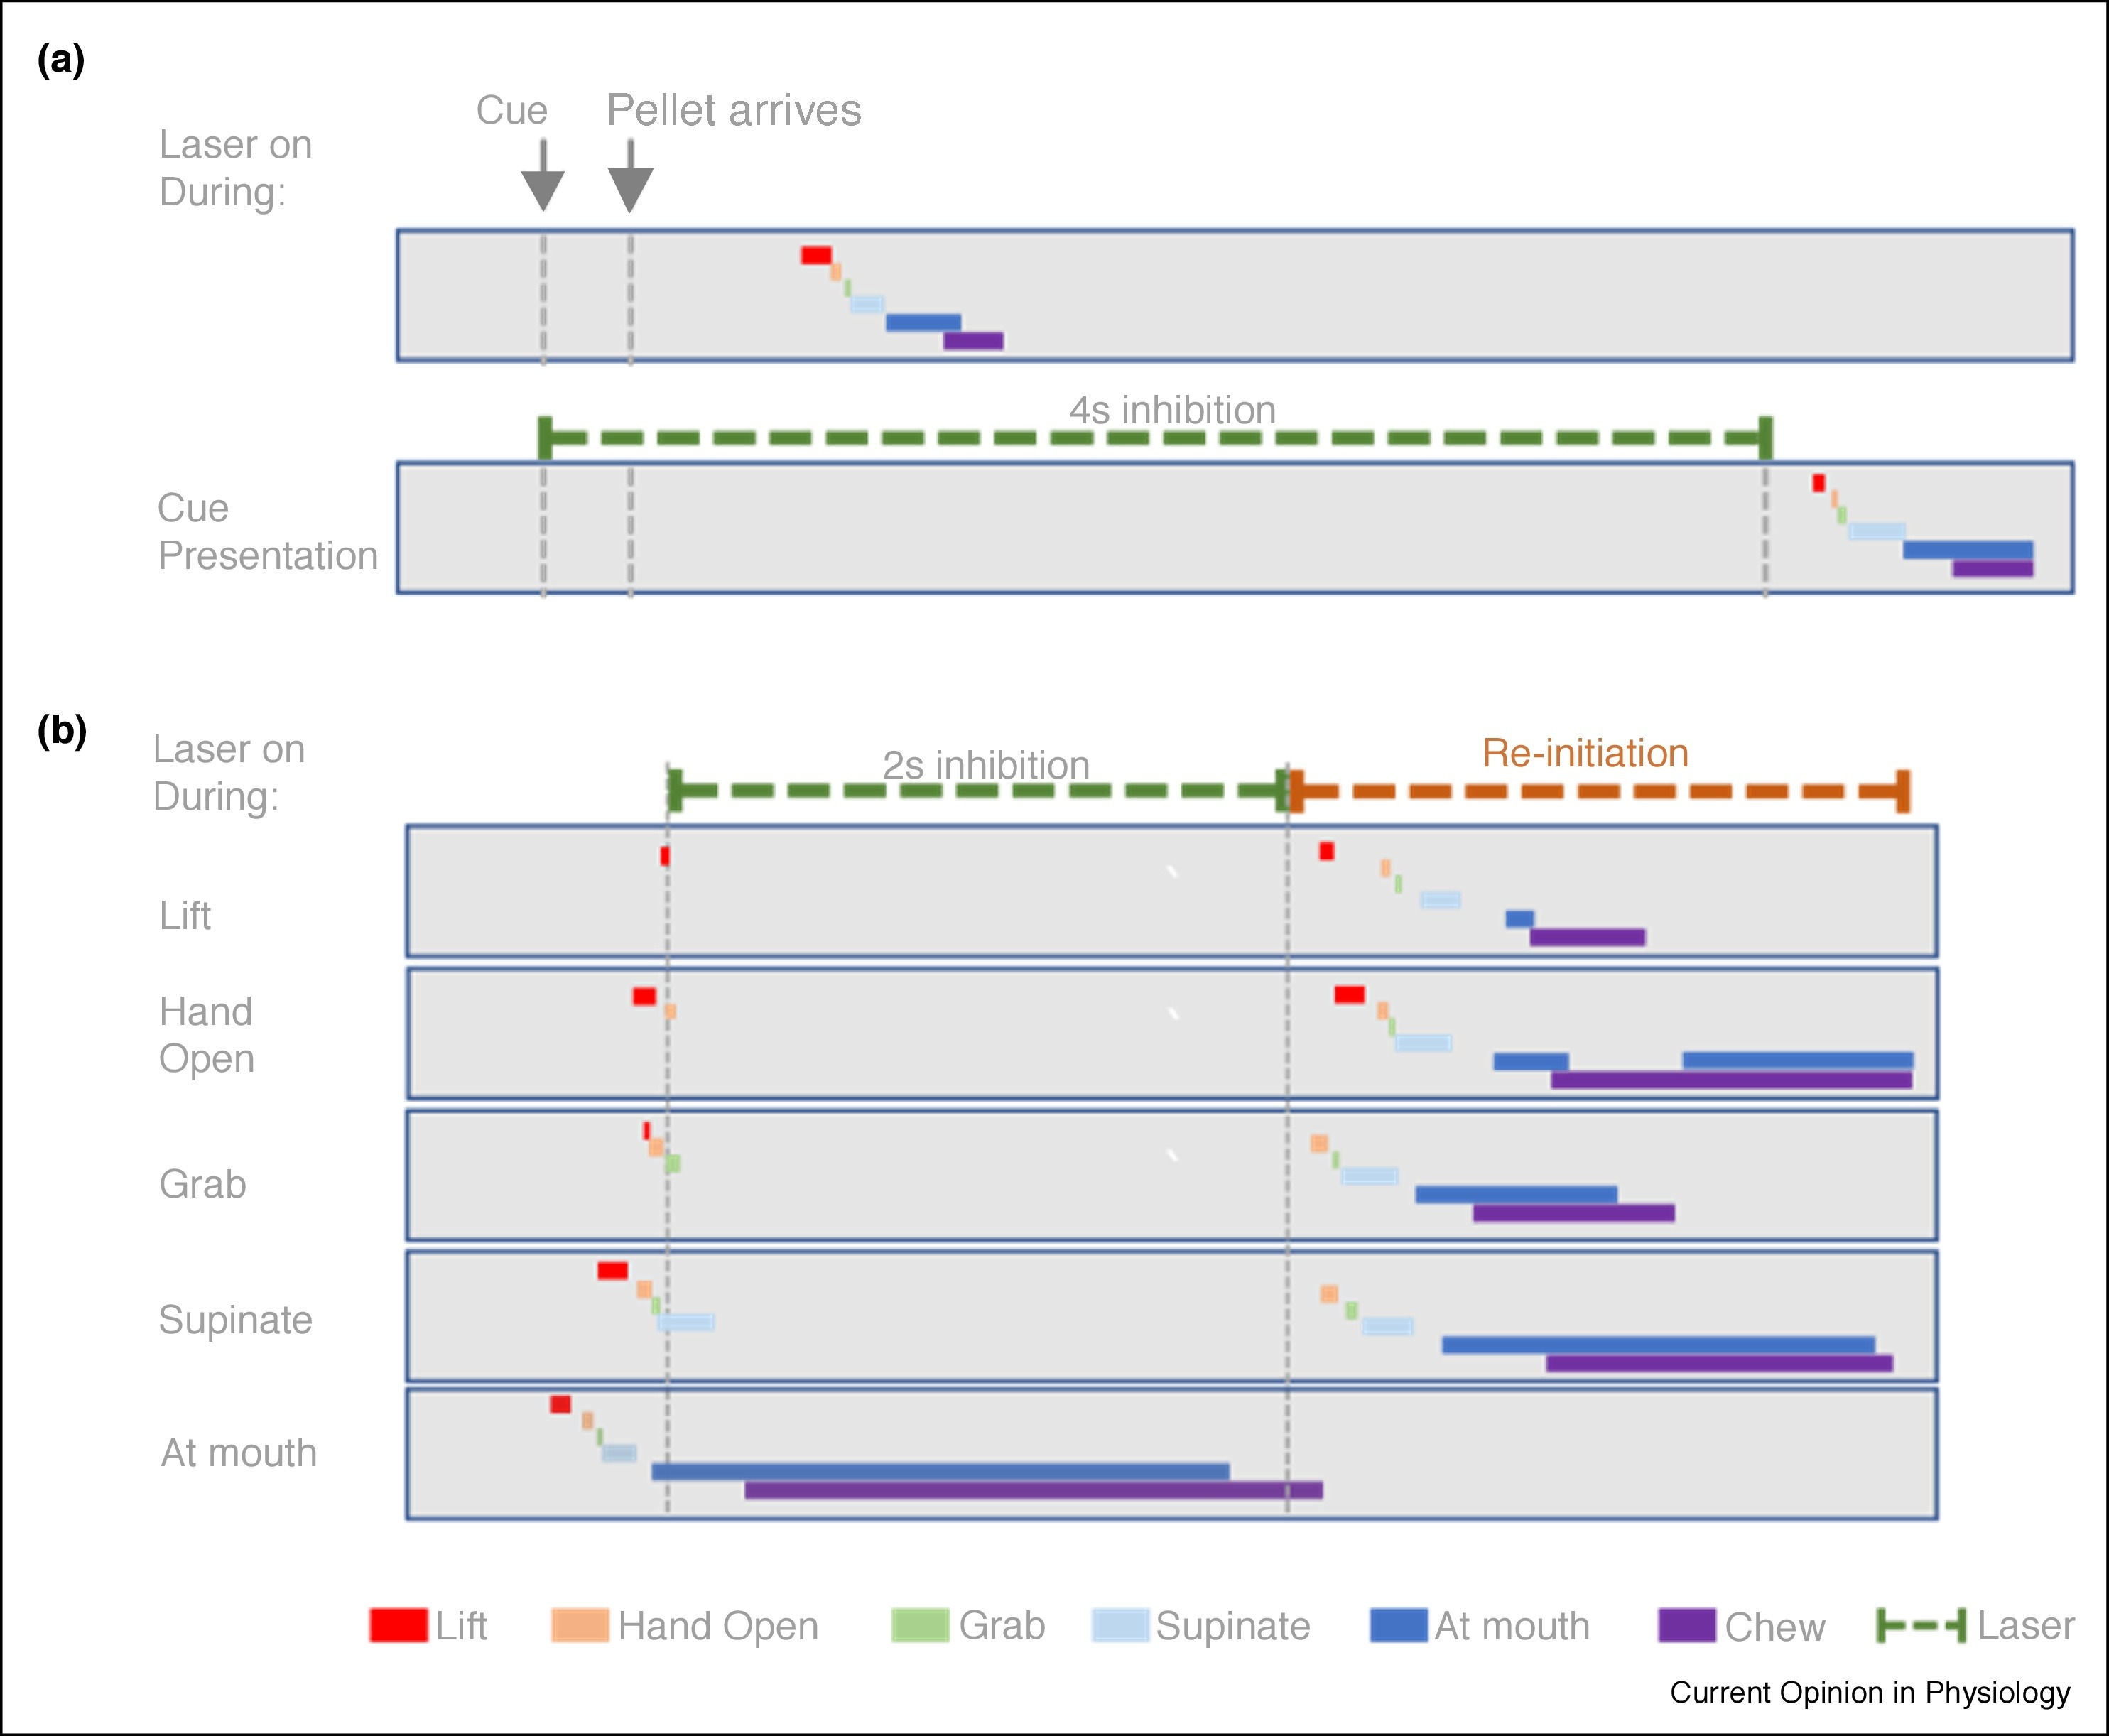
\includegraphics[width=\linewidth]{lin_2021_review_figs/1-s2.0-S2468867320301693-gr1_lrg.jpg}
\caption{\textbf{Dynamic involvement of sensorimotor cortex in well-trained grasping behavior.} \textbf{(a)} Representative trials of multi-stage grasping behavior during control trials (top panel) and sensorimotor cortex inhibition trials (bottom panel). Following the tone-cue presentation, a food pellet was delivered in front of a head-fixed mouse, which would then initiate a grasping movement involving a (∼700 msec) sequence of six sub movements: lift, paw open, grab, supinate, at mouth, and chew. The entire sequence was prevented when the sensorimotor cortex was inhibited optogenetically (indicated by green dashed line) via stimulation of GABAergic inhibitory neurons. The behavior was reinitiated once the laser was turned off. \textbf{(b)} Representative trials in which inhibition was induced at different time-points in the movement. The impact of post-onset perturbations was not immediate, but rather emerged after a delay during which the behavior continued to the beginning of the next component. Cortical perturbations had no impact on impeding hand movement involved in chewing (i.e. at mouth). Note that these are example trials. Durations of some behavioral components are seemingly stretched when sensorimotor cortex was suppressed after behavior being initiated (b), the difference, however, is not statistically significant when all trials were pooled together (cf. Figure 4 of \cite{guo2015a}). The length of color-coded bars denotes the duration of each behavioral component. Figure was adapted from \cite{guo2015a}.}
\label{fig:wrapfig}
\end{figure}



Similarly, the impact of perturbing basolateral amygdalar (BLA) input to the nucleus accumbens (NAcc) in rats trained to make choices between smaller, certain rewards and larger, uncertain rewards (\cite{bercovici2018a}) depends on that perturbation’s specific timing. During trials in which it was applied before animals committed to a choice, the perturbation generally reduced the strength of the rats’ preferences for whichever reward was ‘best’ (i.e. the most rewarding over the long term), regardless of which reward that was (the experimenters were able to change experimental parameters such that the best choice would switch from being the small to the large, or vice versa). If, on the other hand, the BLA→NAcc pathway was inhibited only after uncertain choices that resulted in a lack of reward, the impact was both different and asymmetrical --- the perturbation increased the likelihood of risky choices in subsequent trials (Figure 4.2). The BLA→NAcc connection appears to have different functions at different moments in the task.

\begin{figure}
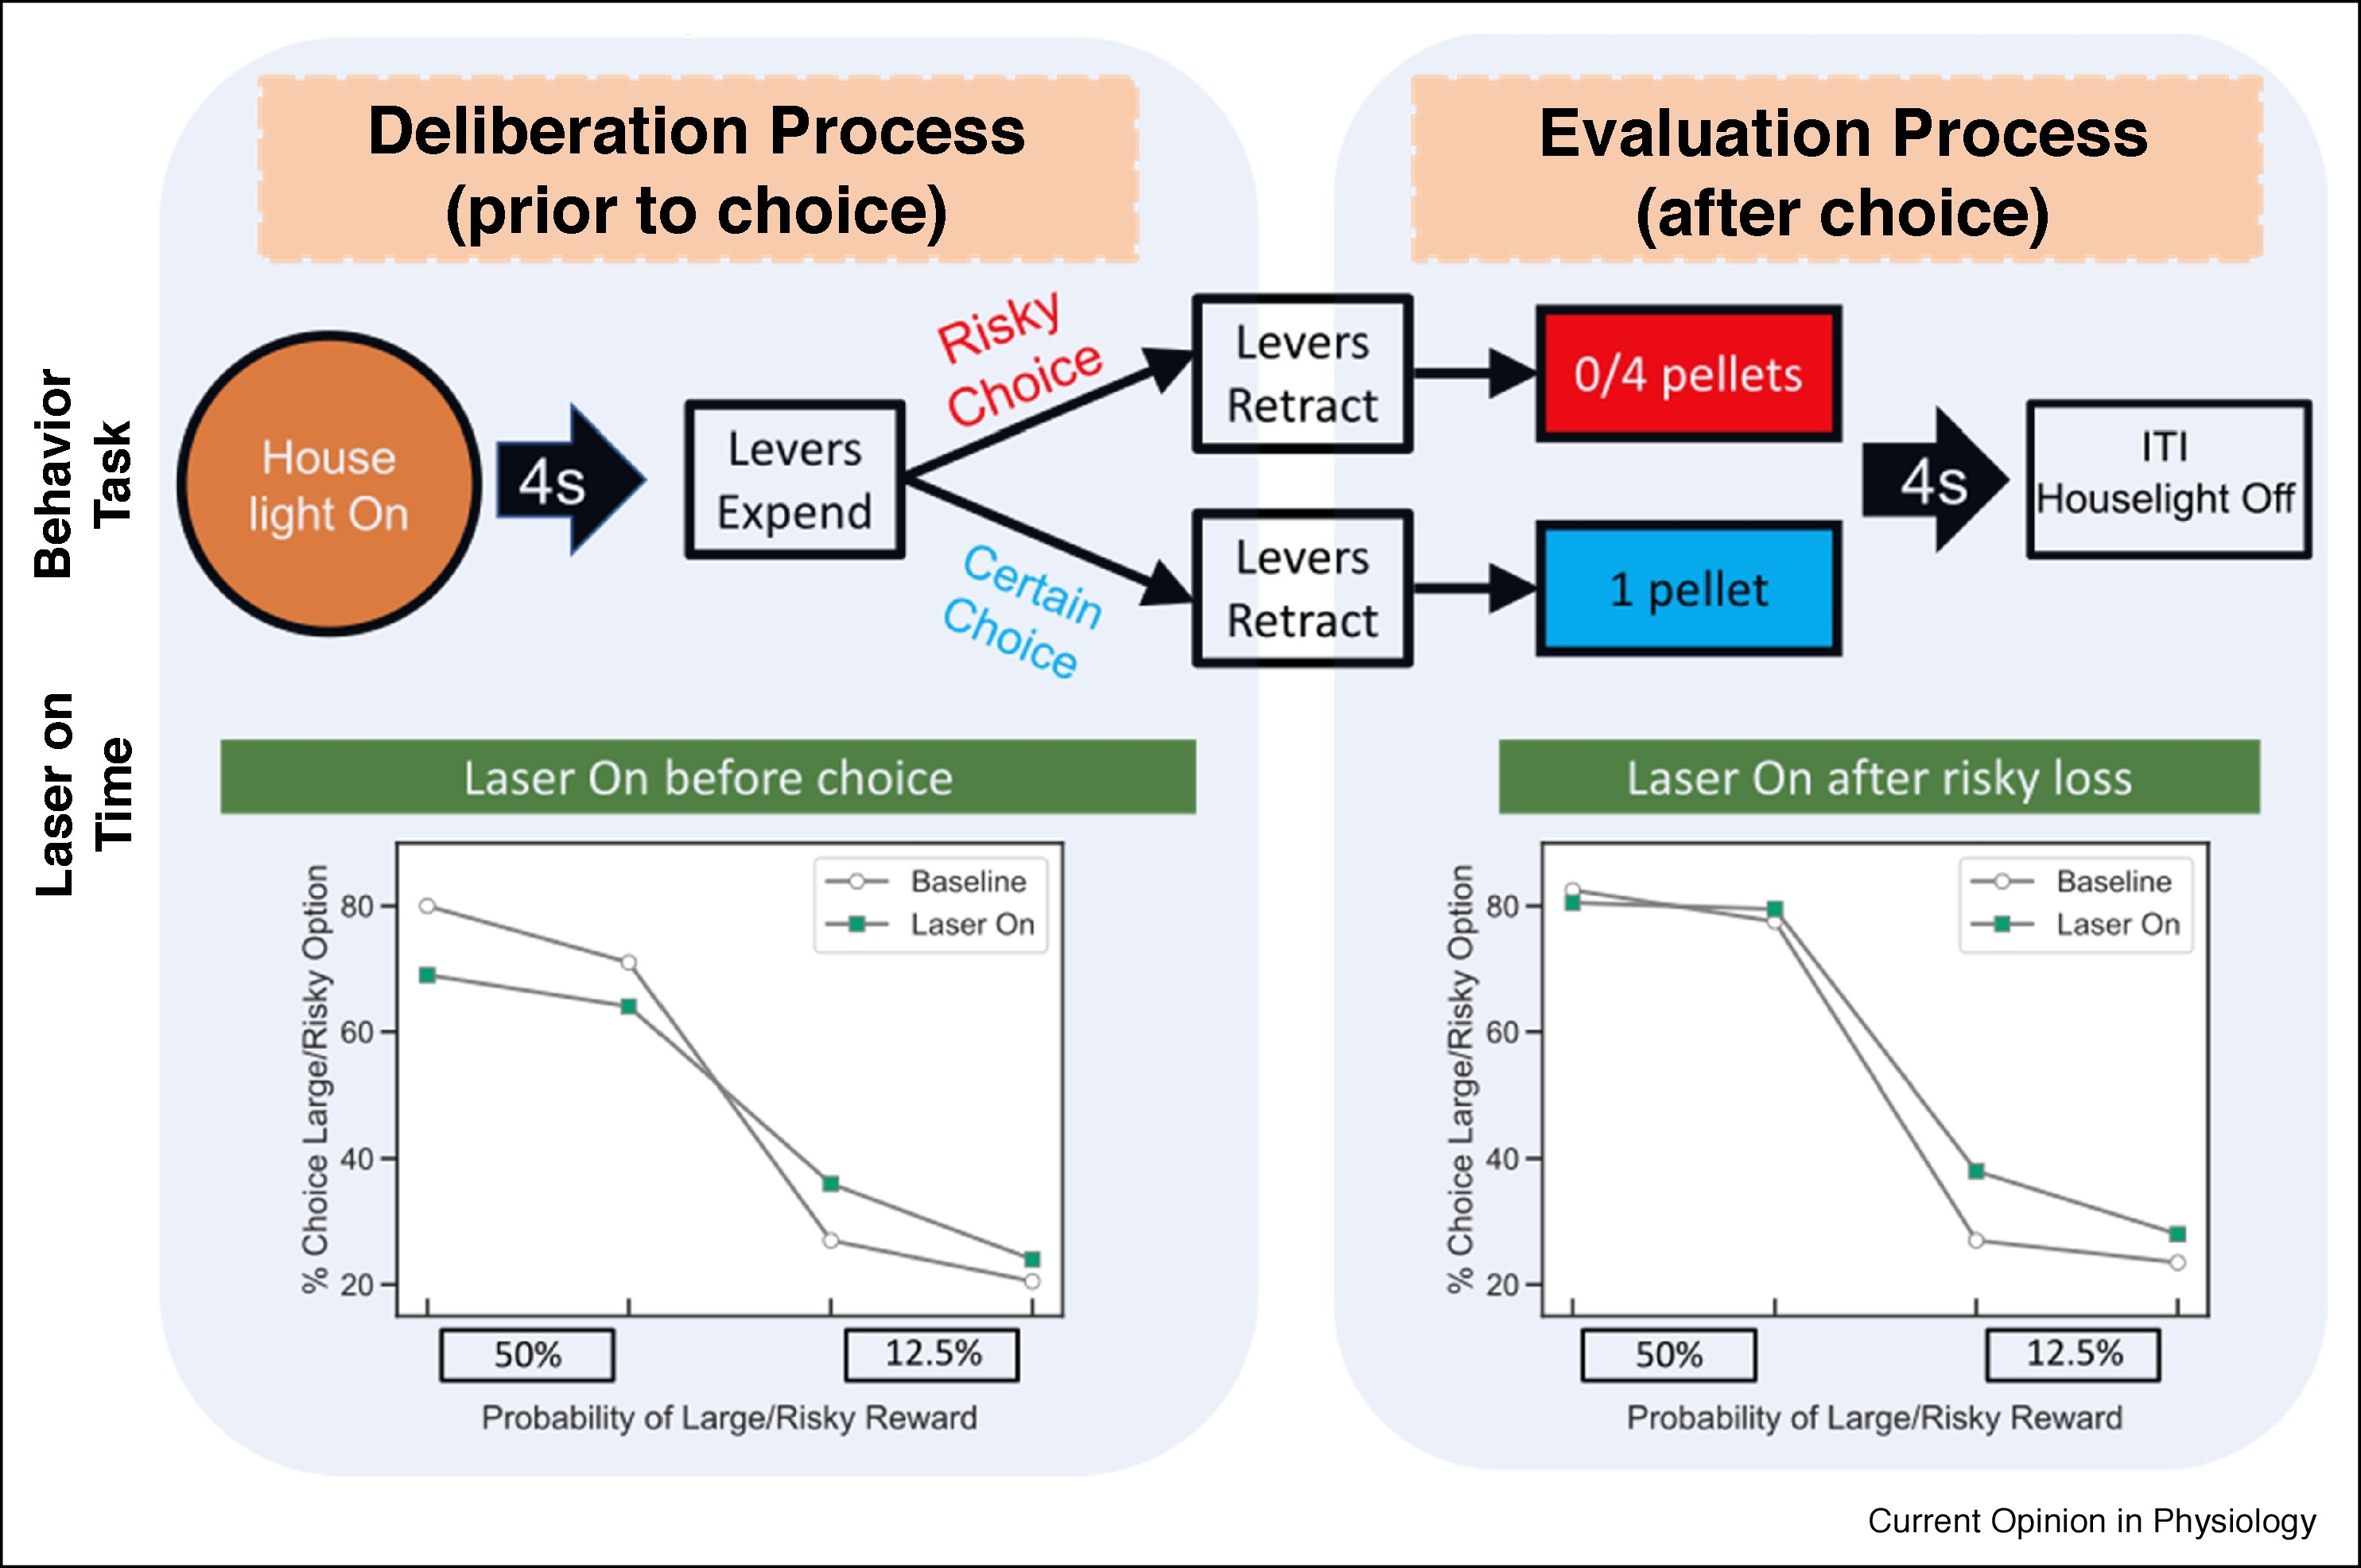
\includegraphics[width=\linewidth]{lin_2021_review_figs/1-s2.0-S2468867320301693-gr2_lrg.jpg}
\caption{\textbf{Functional dynamics of basolateral amygdala (BLA)→nucleus accumbens (NAcc) projection during a decision-making process.} The BLA→NAcc circuitry is involved in decision-making when reward is uncertain. Following acquisition of a probabilistic discounting task, rats received optogenetic inhibition of BLA→NAcc axons (as those axons enter NAcc) either before the choice (during the deliberation process) or after (during the evaluation of choice). The former inhibition significantly reduced subsequent preferences for the optimal choice --- decreasing the likelihood of a risky choice when reward probability was 50\% but decreasing the probability of a safe choice when reward probability was lower (12.5\%). If, meanwhile, BLA→NAcc was inhibited after a choice that led to reward omission, the likelihood of selecting the risky choice increased, but only during the low probability (12.5\%) block. ITI: inter-trial interval. Figure was adapted from \cite{bercovici2018a}.}
\label{fig:wrapfig}
\end{figure}

Of course, in each of the above paradigms, observed firing rates dynamics occur in concert with changes in outward behaviors. To some degree, therefore, it is unsurprising that perturbations of firing at different moments are associated with different changes in specific function, because the animals are doing (at least slightly) different things at different moments. The most risky tests of our thesis (the argument that the function being performed by specific groups of neurons changes across even short stretches of time) will therefore involve neural dynamics that occur in the absence of such outward behavioral dynamics, such as the afore-mentioned cortical coding sequence that spans the gap between the moment that a taste hits the tongue and the moment that discriminative consumption behaviors (ejecting or swallowing) occur.

We have performed this test, taking advantage of the fact that neural ensemble analyses reveal that the transitions between these epochs, and in particular the transition into palatability-related firing (\cite{sadacca2016a}), are sudden and clearly discernible in single trials (c.f. \cite{jones2007a}). The impact of brief (0.5 s) optogenetic inhibition of these neurons has recently been shown to depend exquisitely on the timing of that inhibition: if it begins before the ensemble transition into the palatability state, consumption-related behaviors are greatly delayed; the same perturbation delivered even just a few tens of msec after the transition, however, has no impact on behavior (\cite{mukherjee2019a}) (Figure 4.3). Given the fact that palatability-related firing emerges at different times on different trials, two outwardly identical perturbations (i.e. both occurring at 700 ms after taste delivery) will have predictably different impacts depending on whether neurons have reached the point of coding palatability already on that particular trial. The question of what these neurons do is simply ill-posed --- their function is only defined with reference to a certain time interval and certain pre-existing conditions in the network.

\begin{figure}
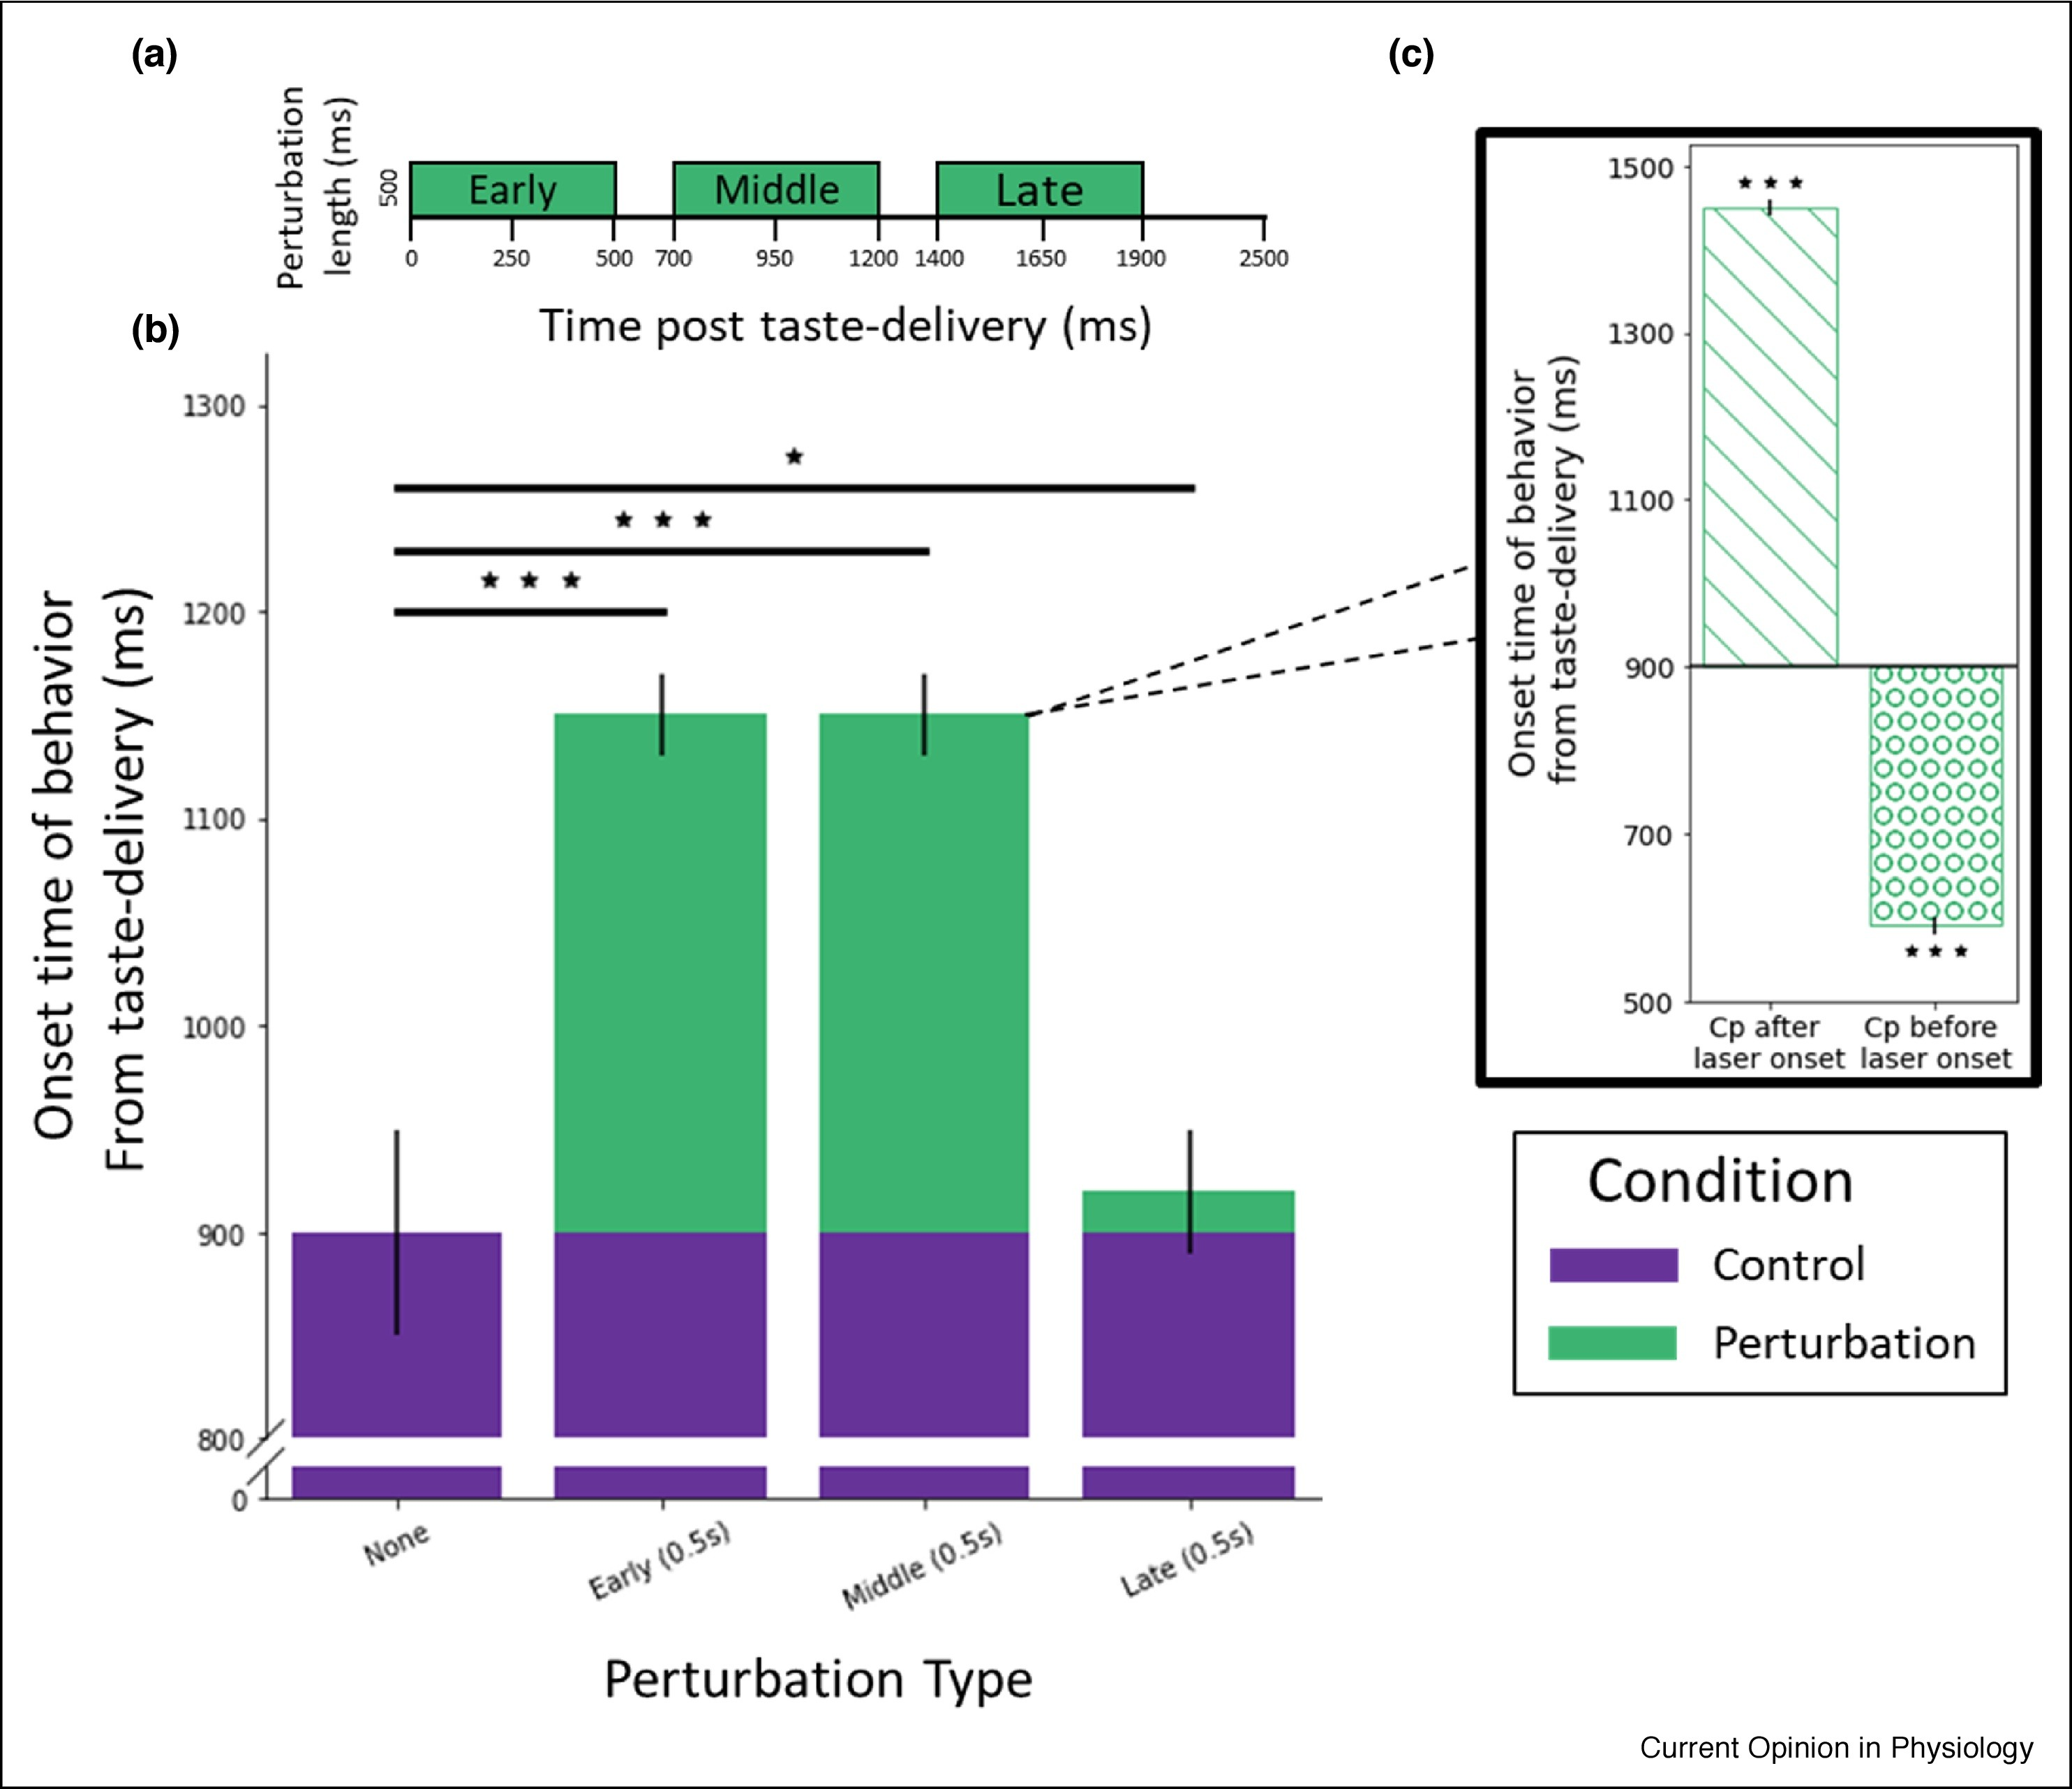
\includegraphics[width=\linewidth]{lin_2021_review_figs/1-s2.0-S2468867320301693-gr3_lrg.jpg}
\caption{\textbf{Behavioral disruption is dependent on precisely timed optogenetic perturbation in gustatory cortex.} (a) Brief (0.5 s) optogenetic inhibition of gustatory cortex was delivered at one of three possible time points post taste-delivery: early (0–0.5 s), middle (0.7–1.2 s), and late (1.4–1.9 s). (b) The bar graph shows the impact (green) of perturbations on latency (y-axis) of gaping (an oral behavior signaling reaching of a rejection decision) to quinine. Purple is the within-session control latency (i.e. on trials with no perturbation). The error bars are the 95\% Bayesian credible intervals (* = p \(<\) 0.05, *** = p \(<\) 0.001). Early and Middle perturbations of cortical taste responses delayed the onset of gaping, while Late perturbations produce only a minor delay in gaping onset. (c) The apparent impact of Middle perturbation on the onset of aversive orofacial behavior shown in (b) is a mix of actual effects, as the true impact depends exquisitely on the state of the ensemble dynamics just before perturbation onset time in that particular trial. The left bar shows the result of the perturbation during trials in which the palatability-related ensemble transition had not occurred before the time of perturbation onset; the right bar represents trials in which palatability-related firing had already occurred before (in some cases, as little as 20 s before) the laser was switched on (i.e, before 0.65 s; adapted from \cite{mukherjee2019a}).}
\label{fig:wrapfig}
\end{figure}

\section{Conclusion}
Studies in which neural responses are quantified only in terms of their average firing rate inevitably under describe the complexity of the activity of neurons embedded in networks. Furthermore, it has long been understood that experiments showing that lesion/inactivation/perturbation of a particular set of neurons impacts behavior fall far short of demonstrating those neurons to be the primary locus of that particular behavior. Neurons that are embedded in interacting networks – networks which ensure multi-responsivity and temporal coding – will also demonstrate exquisite sensitivity to changes imposed upon these networks by any of a number of natural internal or external perturbations.

While it is attractive and simple to think of individual neuron groups and types as having distinct and relatively immutable functions, these above considerations make it unlikely that such theories have a great deal of physiological validity. They instead predict function that is distributed and shifting in concert with firing rate changes, and in accordance with dynamical system principles (\cite{jones2006a,camera2019a,miller2016a}). The studies described here confirm these predictions.

\begin{singlespace}
\printbibliography[title={References}]
\end{singlespace}

\end{refsection}
\begin{refsection}

\chapter{Discussion}

While it is widely recognized that processing of sensory information in the brain is governed by dynamics at multiple timescales, these dynamics have only recently begun to be explored in the context of taste processing. Investigation into the role of multi-region interactions follows a similar trend. While it has been shown that brain regions “up and down” the taste circuit (including the pons, lateral hypothalamus, basolateral amygdala, gustatory cortex, and medial prefrontal cortex) all respond to taste in a dynamic fashion (\cite{katz2001a,fontanini2009a,jezzini2013a,li2013a,baez-santiago2016a}), the work done in this thesis represents the first attempt (to the best of our knowledge) to investigate and characterize interactions between taste regions during processing.

In Chapter 2, we investigate how long-term dynamics on the order of minutes and hours – in the form of sickness caused by gastric malaise- affect taste processing in the gustatory cortex. Despite having only a transient impact on GC LFP spectral properties, sickness induces a long-lasting change in its evoked neural response. It is surprising that there is not persistent "signal” for sickness in GC and it is unlikely that such a signal is not present anywhere in the brain – please note however, that this does not mean that it is the brain that is maintaining such a signal, and such a signal could simply be present in the form of altered spontaneous activity due to input from the viscera. this observation further underpins the idea that GC is not the focus of processing in the taste circuit and that other brain regions are simultaneously playing significant roles. We further see that GC palatability processing is pushed towards a binary choice under sickness rather than a spectrum of hedonic values under normal processing. One may speculate that this increased similarity to BLA’s palatability encoding likely has something to do with changes in BLA-GC functional connectivity during sickness. These points are further discussed in Future Directions section below.

In Chapter 3, we investigate changes in neural dynamics on the order of hundreds of milliseconds and seconds, as well as exploring communication between brain regions involved in taste processing. This investigation tests the long-held belief that the similarity in BLA and GC taste evoked dynamics is due to a direct interaction between them. First we test that BLA population activity contains similar state transitions to GC, which not only suggests that BLA is a similar dynamical system to GC, but also that the two regions could be considered a single system. We then go on to test this assertion by investigation the coordination between BLA and GC. We show that BLA and GC responses are linked at the whole-trial (spike-count correlations), epoch (LFP phase coherence), and state-transition levels, we clearly see that this is not due to a “default” connection between the two regions due to their strong reciprocal connectivity, and that the BLA-GC interaction is dynamic (only appearing significantly around the late [palatability in GC] epoch), which suggests that BLA plays a significant role only later in the evoked taste response. This evidence is further corroborated by previous causal studies (\cite{lin2021a}) showing that while perturbation of the BLA$\rightarrow$GC pathway causes the largest impact on GC neural responses in the 250ms immediately following taste delivery, changes in GC coding are only visible during the palatability epoch. This can likely be explained by the fact that physical disruption of input by the perturbation will cause the largest change when the neural activity is also the highest (it has consistently been shown that that the neural response magnitude is highest immediately following taste delivery [i.e. during the early response epoch] and tapers off over the next 2 seconds), however, the role this projection plays is disturbed specifically during the palatability epoch.

Finally, in Chapter 4, we paint a picture for how neural activity is inherently a dynamic entity, such that the response of a neuron or brain region is ill-characterized without temporal context. This chapter provides a consilience for the previous chapters, discussing how neural responses are influenced by multiple physiological processes and external influences (including sensory input) at multiple timescales. Hence, the same neuron will subserve different computations at different times, and in corollary, will have different network interactions over time as well. Hence, the response of GC neurons changes across trials as governed by the onset of sickness, and zooming into a single trial, we see GC epochal/state dynamics governed by its interactions with BLA (and likely other brain regions as well).

The studies mentioned above, among much other extant research, highlight the importance of investigating how temporal dynamics govern processing in the taste circuit. Given this framework, there are many avenues of research that could be explored to further understand the interregional dynamics that contribute to taste processing and develop a better understanding of the “sources” of neural dynamics at different timescales. An integration of these results into the existing literature and future directions for the work presented in this thesis are reviewed in the section below.

\section{Future Directions}
As mentioned throughout this thesis, a clearer understanding of network interactions in taste processing is still being developed. While pharmacological inhibition and ablation studies have provided important clues to the necessity of brain regions in taste-related learning and normal taste processing, such extreme perturbations can be misleading and not provide a direct test of how the intact taste circuit normally carries out processing. An illustrative example for this case is the fact that rats can still gape despite removal of cortex, which would suggest that cortex plays no role in the generation of gapes. While that is true at face value, and the central pattern generator (CPG) responsible for gaping is certainly located in the brainstem, such an extreme perturbation misses the nuance that despite not being responsible for generating gapes, GC is causally involved in the initiation of the gaping “program” and hence exerts a significant modulatory influence on the CPG. Similarly, we can expect much nuance in the role played by the multitudinous connections within the brain in taste processing.

My suggested avenues for further investigation may be broadly divided into two categories, corresponding to further investigations into the influence of sickness on the taste circuit, and further investigation of network interactions in the taste circuit during taste processing. Additionally, it has been shown that modelling of neural activity across timescales (a.k.a. scale-free modelling) improves prediction accuracy for sensorimotor tasks (\cite{samek2016a,abbaspourazad2021a}); hence, while a direct investigation of ways to scale the gap between the short on long timescales mentioned here will certainly be indispensable for furthering our understanding of processing in the taste circuit, pursuit of this avenue is left for the future.

\subsection{Illness and taste processing}

\smallskip
\noindent \underline{Increased behavioral binarization of food preference under sickness} This would be a confirmatory experiment to test that the increased polarization/binarization of hedonic values as seen in GC under sickness. A simple (possibly naïve) method to carry this out would be to have rats lick to the same tastants given in the experiments in Chapter 2 and undergoing the same experimental conditions (Saline vs LiCl) while in a Brief Access Task rig. Increased similarity (while accounting for any potential floor effects caused by the animal’s illness) in tastants with similar hedonic values would confirm that this is not simply a neural idiosyncracy.

\smallskip
\noindent \underline{Investigating the role of posterior GC in sickness} It is known that posterior gustatory cortex receives more visceral projections and hence may contain stronger signals related to illness, however, differences between anterior and posterior GC have hitherto not been studied. While it seems unlikely that responses in posterior GC would be categorically different, if the influence of illness on neural activity is stronger in posterior GC, it may prove to a better site for further investigation of the influence of illness on taste processing.

\subsection{Functional connectivity dynamics in the taste circuit}
As mentioned above, there has been much investigation of the role of different regions in taste processing and taste-related learning using ablation and bulk pharmacological inhibition. However, the field has only recently begun moving away from these extreme perturbations and begun to investigate the role of connections between regions using targeted inhibition of projection neurons, or (better yet) optogenetic perturbation of axonal projections. However, the realm of “functional connectivity” is still a great unknown in taste processing, where the work presented in Chapter 3 is the first attempt to perform such a characterization, and the studies presented here can be easily extended into many multi-region directions.

\smallskip
\noindent \underline{Changes in other taste regions and in functional connectivity due to illness} While the work in Chapter 2 shows that GC activity is (understandably) altered under the state of illness, the same characterization has yet to be performed for other taste processing regions i.e., what influence does sickness have on activity in BLA or the lateral hypothalamus. Since palatability encoding in BLA is already fairly binary (good vs. bad), does that change (perhaps becoming even more polarized)? One may speculate that the loss of gradation in the GC response under sickness could be due to an increase in connectivity between GC and BLA, such that more nuanced information about tastes from other regions being communicated to GC is mitigated. One may further speculate that since we only observe a transient change in GC LFP during the onset of sickness, but no ongoing change is observed while the animal is sick, that the influence of sickness primarily “resides” in other brain regions (posterior GC, BLA, LH etc) and we are only observing the influence of sickness in GC due to communication of GC with these brain regions. In very liberal wording, the “epicenter” of sickness is a different brain region, yet we observe it’s influence on GC. One can also reasonably expect the communication pathways and dynamics between regions in the taste circuit to be altered due to illness.

\smallskip
\noindent \underline{Ascertaining “top-down” influences exerted by GC} While work in Chapter 3 shows that GC and BLA show coordinated activity, the extent of this evidence is phenomenological. Both GC and BLA almost certainly interact with other brain regions in a dynamic fashion, and it is certainly plausible that the tight state-transition level coordination we see in this study is a general occurrence in multiple regions throughout the taste circuit (i.e., multiple regions in the circuit transition together). Hence, it would be illuminating to causally test the role played by the GCBLA feedback projection. As a first pass, if our hypothesis is correct, we will see that by perturbing this projection we will not only see changes in BLA activity but, since we expect the dyad to be working as a loop, we will also observe an impact on activity in GC. One potential role of this projection could be to communicate “Identity” information (information about taste quality) from GC to BLA which the two regions then collectively transform into palatability. This claim stems from previous evidence showing the pharmacological inhibition of taste thalamus strongly diminishes taste-selectivity (discrimination) in GC starting in the middle epoch (identity epoch: approx. 250-750ms post-stim) in GC, while similar pharmacological inhibition of BLA only has a strong effect on reduction of palatability information in GC during the late epoch (750-1250ms post-stim). This suggests that the thalamic taste pathway supports the first “leg” of the evoked taste response, and this activity then engages the limbic pathway (either through GC or via direct thalamo-amygdalar projections). However, this speculation is largely unconstrained as we know little about the when-and¬-where of coordination between these brain regions, a challenge addressed by the following investigation.

\smallskip
\noindent \underline{Investigating circuit interactions dynamics in passive taste processing} LFP recordings have been previously used to probe the simultaneous evolution of activity in multiple brain regions, and methodologies such as granger causality and vector autoregression have been employed to estimate the magnitude and directionality of influence between these brain regions. However, in many cases, this influence is assumed to be static and long durations of neural activity are homogenously analyzed to assess such connectivity. Certainly, in our case, such a simplification would not be possible, hence more advanced techniques such as auto-regressive Hidden Markov Models or switching Linear Dynamical Systems will need to be employed to estimate state-specific interactions. A suggested set of regions to investigate would include GC, BLA, LH, and Thalamus, which may help further clarify the strength and durations of thalamic vs limbic contributions to taste processing. Such a study may potentially help cast the spotlight on previously unnoticed interactions in the taste circuit and suggest pathways for future causal investigation, and may help to elucidate any isolable roles different regions play in processing.

\section{Conclusion}
As mentioned in the introduction of this thesis, the computational power of neural networks (and hence the brain) is derived from non-linear transformations and long-scale interactions. While we have continued to study the non-linear progressions in taste processing, the long-scale interactions have only just begun to come into focus. The experiments noted above in no way diminish the importance of single-region investigation and analysis, but suggest that similar to hierarchies in temporal timescales observed in the brain, adding multi-region analysis into the hierarchy of taste research will allow a more fruitful interaction between the information gleaned from single-region and multi-region studies.


\printbibliography[title={References}]
\end{refsection}

\end{document}